\documentclass[twoside]{book}

% Packages required by doxygen
\usepackage{fixltx2e}
\usepackage{calc}
\usepackage{doxygen}
\usepackage[export]{adjustbox} % also loads graphicx
\usepackage{graphicx}
\usepackage[utf8]{inputenc}
\usepackage{makeidx}
\usepackage{multicol}
\usepackage{multirow}
\PassOptionsToPackage{warn}{textcomp}
\usepackage{textcomp}
\usepackage[nointegrals]{wasysym}
\usepackage[table]{xcolor}

% Font selection
\usepackage[T1]{fontenc}
\usepackage[scaled=.90]{helvet}
\usepackage{courier}
\usepackage{amssymb}
\usepackage{sectsty}
\renewcommand{\familydefault}{\sfdefault}
\allsectionsfont{%
  \fontseries{bc}\selectfont%
  \color{darkgray}%
}
\renewcommand{\DoxyLabelFont}{%
  \fontseries{bc}\selectfont%
  \color{darkgray}%
}
\newcommand{\+}{\discretionary{\mbox{\scriptsize$\hookleftarrow$}}{}{}}

% Page & text layout
\usepackage{geometry}
\geometry{%
  a4paper,%
  top=2.5cm,%
  bottom=2.5cm,%
  left=2.5cm,%
  right=2.5cm%
}
\tolerance=750
\hfuzz=15pt
\hbadness=750
\setlength{\emergencystretch}{15pt}
\setlength{\parindent}{0cm}
\setlength{\parskip}{0.2cm}
\makeatletter
\renewcommand{\paragraph}{%
  \@startsection{paragraph}{4}{0ex}{-1.0ex}{1.0ex}{%
    \normalfont\normalsize\bfseries\SS@parafont%
  }%
}
\renewcommand{\subparagraph}{%
  \@startsection{subparagraph}{5}{0ex}{-1.0ex}{1.0ex}{%
    \normalfont\normalsize\bfseries\SS@subparafont%
  }%
}
\makeatother

% Headers & footers
\usepackage{fancyhdr}
\pagestyle{fancyplain}
\fancyhead[LE]{\fancyplain{}{\bfseries\thepage}}
\fancyhead[CE]{\fancyplain{}{}}
\fancyhead[RE]{\fancyplain{}{\bfseries\leftmark}}
\fancyhead[LO]{\fancyplain{}{\bfseries\rightmark}}
\fancyhead[CO]{\fancyplain{}{}}
\fancyhead[RO]{\fancyplain{}{\bfseries\thepage}}
\fancyfoot[LE]{\fancyplain{}{}}
\fancyfoot[CE]{\fancyplain{}{}}
\fancyfoot[RE]{\fancyplain{}{\bfseries\scriptsize Generated on Fri Sep 4 2015 12\+:21\+:23 for Tissue Origami by Doxygen }}
\fancyfoot[LO]{\fancyplain{}{\bfseries\scriptsize Generated on Fri Sep 4 2015 12\+:21\+:23 for Tissue Origami by Doxygen }}
\fancyfoot[CO]{\fancyplain{}{}}
\fancyfoot[RO]{\fancyplain{}{}}
\renewcommand{\footrulewidth}{0.4pt}
\renewcommand{\chaptermark}[1]{%
  \markboth{#1}{}%
}
\renewcommand{\sectionmark}[1]{%
  \markright{\thesection\ #1}%
}

% Indices & bibliography
\usepackage{natbib}
\usepackage[titles]{tocloft}
\setcounter{tocdepth}{3}
\setcounter{secnumdepth}{5}
\makeindex

% Hyperlinks (required, but should be loaded last)
\usepackage{ifpdf}
\ifpdf
  \usepackage[pdftex,pagebackref=true]{hyperref}
\else
  \usepackage[ps2pdf,pagebackref=true]{hyperref}
\fi
\hypersetup{%
  colorlinks=true,%
  linkcolor=blue,%
  citecolor=blue,%
  unicode%
}

% Custom commands
\newcommand{\clearemptydoublepage}{%
  \newpage{\pagestyle{empty}\cleardoublepage}%
}


%===== C O N T E N T S =====

\begin{document}

% Titlepage & ToC
\hypersetup{pageanchor=false,
             bookmarks=true,
             bookmarksnumbered=true,
             pdfencoding=unicode
            }
\pagenumbering{roman}
\begin{titlepage}
\vspace*{7cm}
\begin{center}%
{\Large Tissue Origami }\\
\vspace*{1cm}
{\large Generated by Doxygen 1.8.9.1}\\
\vspace*{0.5cm}
{\small Fri Sep 4 2015 12:21:23}\\
\end{center}
\end{titlepage}
\clearemptydoublepage
\tableofcontents
\clearemptydoublepage
\pagenumbering{arabic}
\hypersetup{pageanchor=true}

%--- Begin generated contents ---
\chapter{Hierarchical Index}
\section{Class Hierarchy}
This inheritance list is sorted roughly, but not completely, alphabetically\+:\begin{DoxyCompactList}
\item \contentsline{section}{Growth\+Function\+Base}{\pageref{classGrowthFunctionBase}}{}
\begin{DoxyCompactList}
\item \contentsline{section}{Grid\+Based\+Growth\+Function}{\pageref{classGridBasedGrowthFunction}}{}
\item \contentsline{section}{Ring\+Growth\+Function}{\pageref{classRingGrowthFunction}}{}
\item \contentsline{section}{Uniform\+Growth\+Function}{\pageref{classUniformGrowthFunction}}{}
\end{DoxyCompactList}
\item \contentsline{section}{Model\+Input\+Object}{\pageref{classModelInputObject}}{}
\item \contentsline{section}{Node}{\pageref{classNode}}{}
\item Q\+G\+L\+Widget\begin{DoxyCompactList}
\item \contentsline{section}{G\+L\+Widget}{\pageref{classGLWidget}}{}
\end{DoxyCompactList}
\item Q\+Main\+Window\begin{DoxyCompactList}
\item \contentsline{section}{Main\+Window}{\pageref{classMainWindow}}{}
\end{DoxyCompactList}
\item \contentsline{section}{Reference\+Shape\+Base}{\pageref{classReferenceShapeBase}}{}
\item \contentsline{section}{Shape\+Base}{\pageref{classShapeBase}}{}
\begin{DoxyCompactList}
\item \contentsline{section}{Prism}{\pageref{classPrism}}{}
\item \contentsline{section}{Triangle}{\pageref{classTriangle}}{}
\end{DoxyCompactList}
\item \contentsline{section}{Simulation}{\pageref{classSimulation}}{}
\end{DoxyCompactList}

\chapter{Class Index}
\section{Class List}
Here are the classes, structs, unions and interfaces with brief descriptions\+:\begin{DoxyCompactList}
\item\contentsline{section}{\hyperlink{classAnalysis}{Analysis} }{\pageref{classAnalysis}}{}
\item\contentsline{section}{\hyperlink{classCellMigration}{Cell\+Migration} }{\pageref{classCellMigration}}{}
\item\contentsline{section}{\hyperlink{classGLWidget}{G\+L\+Widget} }{\pageref{classGLWidget}}{}
\item\contentsline{section}{\hyperlink{classGridBasedGrowthFunction}{Grid\+Based\+Growth\+Function} }{\pageref{classGridBasedGrowthFunction}}{}
\item\contentsline{section}{\hyperlink{classGrowthFunctionBase}{Growth\+Function\+Base} }{\pageref{classGrowthFunctionBase}}{}
\item\contentsline{section}{\hyperlink{classLumen}{Lumen} }{\pageref{classLumen}}{}
\item\contentsline{section}{\hyperlink{classMainWindow}{Main\+Window} }{\pageref{classMainWindow}}{}
\item\contentsline{section}{\hyperlink{classmarkerEllipseBasedShapeChangeFunction}{marker\+Ellipse\+Based\+Shape\+Change\+Function} }{\pageref{classmarkerEllipseBasedShapeChangeFunction}}{}
\item\contentsline{section}{\hyperlink{classModelInputObject}{Model\+Input\+Object} }{\pageref{classModelInputObject}}{}
\item\contentsline{section}{\hyperlink{classMuscleFibres}{Muscle\+Fibres} }{\pageref{classMuscleFibres}}{}
\item\contentsline{section}{\hyperlink{classMyosinFunction}{Myosin\+Function} }{\pageref{classMyosinFunction}}{}
\item\contentsline{section}{\hyperlink{classNewtonRaphsonSolver}{Newton\+Raphson\+Solver} }{\pageref{classNewtonRaphsonSolver}}{}
\item\contentsline{section}{\hyperlink{classNode}{Node} }{\pageref{classNode}}{}
\item\contentsline{section}{\hyperlink{classPrism}{Prism} }{\pageref{classPrism}}{}
\item\contentsline{section}{\hyperlink{classRandomGenerator}{Random\+Generator} }{\pageref{classRandomGenerator}}{}
\item\contentsline{section}{\hyperlink{classReferenceShapeBase}{Reference\+Shape\+Base} }{\pageref{classReferenceShapeBase}}{}
\item\contentsline{section}{\hyperlink{classRingGrowthFunction}{Ring\+Growth\+Function} }{\pageref{classRingGrowthFunction}}{}
\item\contentsline{section}{\hyperlink{classShapeBase}{Shape\+Base} }{\pageref{classShapeBase}}{}
\item\contentsline{section}{\hyperlink{classSimulation}{Simulation} }{\pageref{classSimulation}}{}
\item\contentsline{section}{\hyperlink{classUniformGrowthFunction}{Uniform\+Growth\+Function} }{\pageref{classUniformGrowthFunction}}{}
\item\contentsline{section}{\hyperlink{classUniformShapeChangeFunction}{Uniform\+Shape\+Change\+Function} }{\pageref{classUniformShapeChangeFunction}}{}
\end{DoxyCompactList}

\chapter{Class Documentation}
\hypertarget{classGLWidget}{}\section{G\+L\+Widget Class Reference}
\label{classGLWidget}\index{G\+L\+Widget@{G\+L\+Widget}}


{\ttfamily \#include $<$G\+L\+Widget.\+h$>$}

Inheritance diagram for G\+L\+Widget\+:\begin{figure}[H]
\begin{center}
\leavevmode
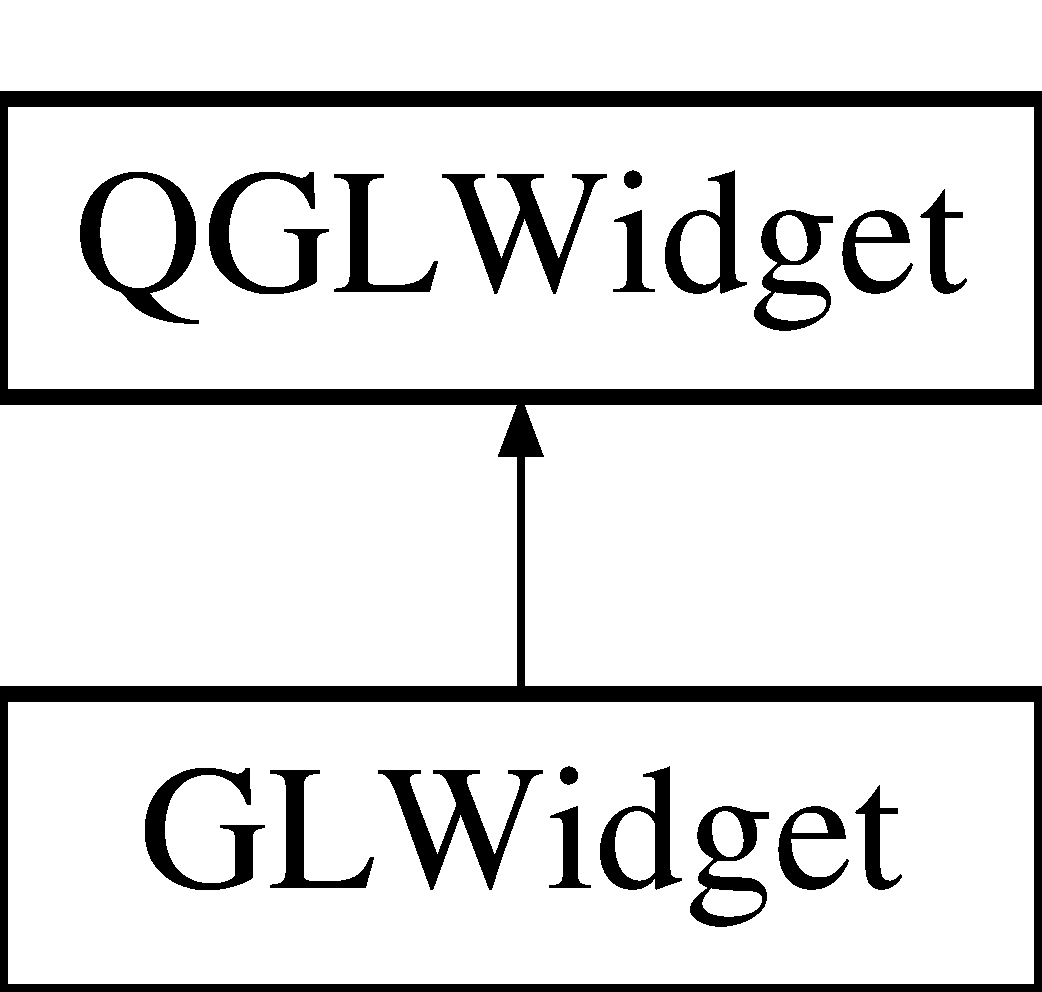
\includegraphics[height=2.000000cm]{classGLWidget}
\end{center}
\end{figure}
\subsection*{Signals}
\begin{DoxyCompactItemize}
\item 
\hypertarget{classGLWidget_a031d84e410b07e5c8afca4ab11e06c54}{}void {\bfseries Selected\+Item\+Changed} ()\label{classGLWidget_a031d84e410b07e5c8afca4ab11e06c54}

\item 
\hypertarget{classGLWidget_a628dd262f28dda97912e2f5d61eb8c6a}{}void {\bfseries Need\+To\+Clear\+Manual\+Element\+Selection} ()\label{classGLWidget_a628dd262f28dda97912e2f5d61eb8c6a}

\item 
\hypertarget{classGLWidget_a7bbc4801f4a079987dd5e7f46137b314}{}void {\bfseries Need\+To\+Clear\+Manual\+Node\+Selection} ()\label{classGLWidget_a7bbc4801f4a079987dd5e7f46137b314}

\end{DoxyCompactItemize}
\subsection*{Public Member Functions}
\begin{DoxyCompactItemize}
\item 
\hypertarget{classGLWidget_ab79c391c86de1ffb76f6950b49d82c0c}{}{\bfseries G\+L\+Widget} (Q\+Widget $\ast$parent=0)\label{classGLWidget_ab79c391c86de1ffb76f6950b49d82c0c}

\item 
\hypertarget{classGLWidget_ade3142625c1bfda0576e419b176cf8b1}{}Q\+Size {\bfseries minimum\+Size\+Hint} () const \label{classGLWidget_ade3142625c1bfda0576e419b176cf8b1}

\item 
\hypertarget{classGLWidget_a57698bc426052845b43a135a13540154}{}Q\+Size {\bfseries size\+Hint} () const \label{classGLWidget_a57698bc426052845b43a135a13540154}

\item 
\hypertarget{classGLWidget_ad425870ac081f6814c5bdb794e6e4c21}{}void {\bfseries manual\+Element\+Selection} (int i)\label{classGLWidget_ad425870ac081f6814c5bdb794e6e4c21}

\item 
\hypertarget{classGLWidget_a21f7a00a668f6ab6c5a9b1491e30c43e}{}void {\bfseries manual\+Node\+Selection} (int i)\label{classGLWidget_a21f7a00a668f6ab6c5a9b1491e30c43e}

\item 
\hypertarget{classGLWidget_ad569f9af7f5bbbfee5f1810d07107f20}{}void {\bfseries update\+Clipping} ()\label{classGLWidget_ad569f9af7f5bbbfee5f1810d07107f20}

\item 
\hypertarget{classGLWidget_adf09146230a2acda5a955acf59fbc653}{}void {\bfseries update\+To\+Top\+View} ()\label{classGLWidget_adf09146230a2acda5a955acf59fbc653}

\item 
\hypertarget{classGLWidget_ab4dcb3e931649a5f1edb6c6cede31075}{}void {\bfseries update\+To\+Front\+View} ()\label{classGLWidget_ab4dcb3e931649a5f1edb6c6cede31075}

\item 
\hypertarget{classGLWidget_a4930d77748cd175e349194da489c12d5}{}void {\bfseries update\+To\+Side\+View} ()\label{classGLWidget_a4930d77748cd175e349194da489c12d5}

\item 
\hypertarget{classGLWidget_afa3014a464a473c9ba62b22720f2d6fd}{}void {\bfseries update\+To\+Perspective\+View} ()\label{classGLWidget_afa3014a464a473c9ba62b22720f2d6fd}

\item 
\hypertarget{classGLWidget_af9b7537315485a04dd848ee62ac60b1e}{}void {\bfseries draw\+Points\+For\+Display} ()\label{classGLWidget_af9b7537315485a04dd848ee62ac60b1e}

\end{DoxyCompactItemize}
\subsection*{Public Attributes}
\begin{DoxyCompactItemize}
\item 
\hypertarget{classGLWidget_a9d11c25470e7e6d635d90b9605d54a2e}{}\hyperlink{classSimulation}{Simulation} $\ast$ {\bfseries Sim01}\label{classGLWidget_a9d11c25470e7e6d635d90b9605d54a2e}

\item 
\hypertarget{classGLWidget_a37fa0d9c8bfb720f550365da0aefccc7}{}bool {\bfseries Item\+Selected}\label{classGLWidget_a37fa0d9c8bfb720f550365da0aefccc7}

\item 
\hypertarget{classGLWidget_a67bf1bb7f19922f4ccb6728f339920e4}{}string {\bfseries Selected\+Item\+Name}\label{classGLWidget_a67bf1bb7f19922f4ccb6728f339920e4}

\item 
\hypertarget{classGLWidget_a908e8a53461c09eacf8d82d78d0a84d3}{}int {\bfseries Selected\+Item\+Index}\label{classGLWidget_a908e8a53461c09eacf8d82d78d0a84d3}

\item 
\hypertarget{classGLWidget_ab9d645f750345fde45fea123debb7f27}{}bool {\bfseries Manual\+Node\+Selection}\label{classGLWidget_ab9d645f750345fde45fea123debb7f27}

\item 
\hypertarget{classGLWidget_a4dac57a8924f1f9feb6d6bae75fe6d13}{}int {\bfseries Manual\+Selected\+Node\+Id}\label{classGLWidget_a4dac57a8924f1f9feb6d6bae75fe6d13}

\item 
\hypertarget{classGLWidget_a314984029a390e02a2d4235c5c2741a5}{}bool {\bfseries Display\+Strains}\label{classGLWidget_a314984029a390e02a2d4235c5c2741a5}

\item 
\hypertarget{classGLWidget_a753550713effac7b997844f2759c6129}{}float {\bfseries Display\+Strain\+Range} \mbox{[}2\mbox{]}\label{classGLWidget_a753550713effac7b997844f2759c6129}

\item 
\hypertarget{classGLWidget_ae95a720ff47f77ab05229d6502223c6f}{}int {\bfseries Strain\+To\+Display}\label{classGLWidget_ae95a720ff47f77ab05229d6502223c6f}

\item 
\hypertarget{classGLWidget_a9a990de1ec4c0e18778611cb0159eac8}{}bool {\bfseries Display\+Pys\+Prop}\label{classGLWidget_a9a990de1ec4c0e18778611cb0159eac8}

\item 
\hypertarget{classGLWidget_a478ab24d1ae3c646f40afedb72b725ae}{}int {\bfseries Pys\+Prop\+To\+Display}\label{classGLWidget_a478ab24d1ae3c646f40afedb72b725ae}

\item 
\hypertarget{classGLWidget_a04ab3aa5ad2078d0a495379907eb63ae}{}float {\bfseries Display\+Pys\+Prop\+Range} \mbox{[}6\mbox{]}\mbox{[}2\mbox{]}\label{classGLWidget_a04ab3aa5ad2078d0a495379907eb63ae}

\item 
\hypertarget{classGLWidget_a9bad9c8e609c86125850e2f83350d704}{}float {\bfseries Display\+Pys\+Prop\+Bounds} \mbox{[}6\mbox{]}\mbox{[}4\mbox{]}\label{classGLWidget_a9bad9c8e609c86125850e2f83350d704}

\item 
\hypertarget{classGLWidget_a93d20b91ca92dcd761870fb05291d9cd}{}int {\bfseries Display\+Pys\+Prop\+Decimals} \mbox{[}6\mbox{]}\label{classGLWidget_a93d20b91ca92dcd761870fb05291d9cd}

\item 
\hypertarget{classGLWidget_ae93978d9d5561027cf8697694ca695d3}{}float {\bfseries Display\+Pys\+Prop\+Steps} \mbox{[}6\mbox{]}\label{classGLWidget_ae93978d9d5561027cf8697694ca695d3}

\item 
\hypertarget{classGLWidget_ac238abe591ebaf2aa26a65378a65ce0f}{}vector$<$ Q\+String $>$ {\bfseries Selected\+Pos}\label{classGLWidget_ac238abe591ebaf2aa26a65378a65ce0f}

\item 
\hypertarget{classGLWidget_a358fbf9622862b7fd18a5eafca90aaf2}{}vector$<$ Q\+String $>$ {\bfseries Selected\+Id}\label{classGLWidget_a358fbf9622862b7fd18a5eafca90aaf2}

\item 
\hypertarget{classGLWidget_a66ce8db8191fcb7bac6e7d819bb30b95}{}bool {\bfseries draw\+Net\+Forces}\label{classGLWidget_a66ce8db8191fcb7bac6e7d819bb30b95}

\item 
\hypertarget{classGLWidget_a993ff9e84e7837735b14743a10cd6ddd}{}bool {\bfseries draw\+Myosin\+Forces}\label{classGLWidget_a993ff9e84e7837735b14743a10cd6ddd}

\item 
\hypertarget{classGLWidget_ab9f882d19b598a85dc5da6201681376a}{}int {\bfseries Myosin\+To\+Display}\label{classGLWidget_ab9f882d19b598a85dc5da6201681376a}

\item 
\hypertarget{classGLWidget_a667580ff60b536f89e8b693c6f043868}{}bool {\bfseries draw\+Packing\+Forces}\label{classGLWidget_a667580ff60b536f89e8b693c6f043868}

\item 
\hypertarget{classGLWidget_ae57adc8b63690ebf5bf1d3e4ab35ae44}{}bool {\bfseries draw\+Velocities}\label{classGLWidget_ae57adc8b63690ebf5bf1d3e4ab35ae44}

\item 
\hypertarget{classGLWidget_a1198d8100d85dec3c9a106081d1465df}{}bool {\bfseries draw\+Tissue\+Scale\+Bar}\label{classGLWidget_a1198d8100d85dec3c9a106081d1465df}

\item 
\hypertarget{classGLWidget_af59fc963b9eaf559dfd0ad41cf88dac0}{}bool {\bfseries draw\+Peripodial\+Membrane}\label{classGLWidget_af59fc963b9eaf559dfd0ad41cf88dac0}

\item 
\hypertarget{classGLWidget_a404f4d4130a0c3ea84aeaaac6adb618b}{}bool {\bfseries draw\+Columnar}\label{classGLWidget_a404f4d4130a0c3ea84aeaaac6adb618b}

\item 
\hypertarget{classGLWidget_ac011fc6341a41ec96b9a2a332e223617}{}bool {\bfseries Perspective\+View}\label{classGLWidget_ac011fc6341a41ec96b9a2a332e223617}

\item 
\hypertarget{classGLWidget_a2f10bf15fc043faacc7aa533ca31c3ee}{}bool {\bfseries display\+Bounding\+Box}\label{classGLWidget_a2f10bf15fc043faacc7aa533ca31c3ee}

\item 
\hypertarget{classGLWidget_a16bec7573f51d68f7606c13d258fdff2}{}bool {\bfseries display\+Pipette}\label{classGLWidget_a16bec7573f51d68f7606c13d258fdff2}

\item 
\hypertarget{classGLWidget_a24d8815d6f656844dabf893a09bee5d6}{}double {\bfseries x\+Clip}\label{classGLWidget_a24d8815d6f656844dabf893a09bee5d6}

\item 
\hypertarget{classGLWidget_a688447afa71d6b4b004a933991f2d8de}{}double {\bfseries y\+Clip}\label{classGLWidget_a688447afa71d6b4b004a933991f2d8de}

\item 
\hypertarget{classGLWidget_a3deec68705f88f3d1653b380f8c918b3}{}double {\bfseries z\+Clip}\label{classGLWidget_a3deec68705f88f3d1653b380f8c918b3}

\item 
\hypertarget{classGLWidget_a50707fe8f3eb2f48a541094af67c0e2b}{}bool {\bfseries draw\+Symmetricity}\label{classGLWidget_a50707fe8f3eb2f48a541094af67c0e2b}

\end{DoxyCompactItemize}
\subsection*{Protected Member Functions}
\begin{DoxyCompactItemize}
\item 
\hypertarget{classGLWidget_a7fab13e8cc9fc0730ca54c08b2c923a7}{}void {\bfseries initialize\+G\+L} ()\label{classGLWidget_a7fab13e8cc9fc0730ca54c08b2c923a7}

\item 
\hypertarget{classGLWidget_a640b5570cb2b37724fd5b58a77339c5e}{}void {\bfseries paint\+G\+L} ()\label{classGLWidget_a640b5570cb2b37724fd5b58a77339c5e}

\item 
\hypertarget{classGLWidget_ac0d2a8ecf60907a81c0d73475d851025}{}void {\bfseries resize\+G\+L} (int width, int height)\label{classGLWidget_ac0d2a8ecf60907a81c0d73475d851025}

\item 
\hypertarget{classGLWidget_ab144cc8064c1bbf6d0ef0646ca0bd06c}{}void {\bfseries mouse\+Press\+Event} (Q\+Mouse\+Event $\ast$event)\label{classGLWidget_ab144cc8064c1bbf6d0ef0646ca0bd06c}

\item 
\hypertarget{classGLWidget_ab992c4c25439a5ef23031991015451c1}{}void {\bfseries mouse\+Release\+Event} (Q\+Mouse\+Event $\ast$event)\label{classGLWidget_ab992c4c25439a5ef23031991015451c1}

\item 
\hypertarget{classGLWidget_a9043bac13d6f0a5307ea5c7f9b3caa50}{}void {\bfseries mouse\+Move\+Event} (Q\+Mouse\+Event $\ast$event)\label{classGLWidget_a9043bac13d6f0a5307ea5c7f9b3caa50}

\item 
\hypertarget{classGLWidget_a5702a23f7cf42d05fe55a417d810a4b6}{}void {\bfseries wheel\+Event} (Q\+Wheel\+Event $\ast$event)\label{classGLWidget_a5702a23f7cf42d05fe55a417d810a4b6}

\item 
\hypertarget{classGLWidget_af102973086f831f0a27b3458c57bb337}{}void {\bfseries Object\+Selection} (Q\+Point Last\+Pos)\label{classGLWidget_af102973086f831f0a27b3458c57bb337}

\item 
\hypertarget{classGLWidget_a4aba027a507e84b880acd641275165d4}{}void {\bfseries reset\+Item\+Selection\+Info} (int source)\label{classGLWidget_a4aba027a507e84b880acd641275165d4}

\item 
\hypertarget{classGLWidget_a7fe217738ad7d4c54caa575068641234}{}void {\bfseries find\+Element} ()\label{classGLWidget_a7fe217738ad7d4c54caa575068641234}

\item 
\hypertarget{classGLWidget_aa1c349f897d0fee1163abba8fd39995c}{}bool {\bfseries find\+Element} (int i)\label{classGLWidget_aa1c349f897d0fee1163abba8fd39995c}

\item 
\hypertarget{classGLWidget_a7ff762be5c3562616b6cc4bc6d6b6683}{}bool {\bfseries find\+Node} (int i)\label{classGLWidget_a7ff762be5c3562616b6cc4bc6d6b6683}

\item 
\hypertarget{classGLWidget_afc09ab8fa7a8163ca1b69e7953e33dc4}{}void {\bfseries get\+Colour\+Of\+Point} (Q\+Point Last\+Pos)\label{classGLWidget_afc09ab8fa7a8163ca1b69e7953e33dc4}

\item 
\hypertarget{classGLWidget_a218fadfeda519fd8a120b702f04771c8}{}void {\bfseries draw\+For\+Picking} ()\label{classGLWidget_a218fadfeda519fd8a120b702f04771c8}

\item 
\hypertarget{classGLWidget_a1f66af8462807ed77b878cba3e60bbb9}{}void {\bfseries generate3\+D\+Object} ()\label{classGLWidget_a1f66af8462807ed77b878cba3e60bbb9}

\item 
\hypertarget{classGLWidget_a30be9e529d717552be70cbad097d99e8}{}void {\bfseries initialise\+Node\+Colour\+List} ()\label{classGLWidget_a30be9e529d717552be70cbad097d99e8}

\item 
\hypertarget{classGLWidget_a8597de4600272fb1720641fd1990f153}{}bool {\bfseries check\+If\+Drawing\+Element} (int i)\label{classGLWidget_a8597de4600272fb1720641fd1990f153}

\item 
\hypertarget{classGLWidget_a95a5dc2578aeaf9df7127c0af7d1a531}{}bool {\bfseries check\+If\+Drawing\+Element\+Symmetric} (int i, bool symmetric\+X, bool symmetric\+Y)\label{classGLWidget_a95a5dc2578aeaf9df7127c0af7d1a531}

\item 
\hypertarget{classGLWidget_a4e843eda050d818414f6c722f806cf88}{}bool {\bfseries check\+If\+Drawing\+Node} (int i)\label{classGLWidget_a4e843eda050d818414f6c722f806cf88}

\item 
\hypertarget{classGLWidget_aa85fc1e14fb11fc62ce93cc72ffb5a61}{}void {\bfseries draw\+Element} (int i, bool picking)\label{classGLWidget_aa85fc1e14fb11fc62ce93cc72ffb5a61}

\item 
\hypertarget{classGLWidget_ada0503af64f483c91e342ba5c3dcef49}{}void {\bfseries highlight\+Element} (int i)\label{classGLWidget_ada0503af64f483c91e342ba5c3dcef49}

\item 
\hypertarget{classGLWidget_addb75eed990f0b943d47009f14e8a3de}{}void {\bfseries highlight\+Node} (int i)\label{classGLWidget_addb75eed990f0b943d47009f14e8a3de}

\item 
\hypertarget{classGLWidget_a7be96b028f099e61dfbc75254316c078}{}void {\bfseries draw\+Reference\+Element} (int i)\label{classGLWidget_a7be96b028f099e61dfbc75254316c078}

\item 
\hypertarget{classGLWidget_a523f68e2bf91f762bbd4fb5ab734e737}{}void {\bfseries draw\+Prism} (int i, bool symmetric\+X, bool symmetric\+Y)\label{classGLWidget_a523f68e2bf91f762bbd4fb5ab734e737}

\item 
\hypertarget{classGLWidget_a61c80b66b9686c4325dec480f6d3eef9}{}void {\bfseries draw\+Triangle} (int i)\label{classGLWidget_a61c80b66b9686c4325dec480f6d3eef9}

\item 
\hypertarget{classGLWidget_a36c00f9f2aec8eff1291efd1416be16e}{}void {\bfseries draw\+Prism\+For\+Picking} (int i)\label{classGLWidget_a36c00f9f2aec8eff1291efd1416be16e}

\item 
\hypertarget{classGLWidget_a1b670bed499c7bb756cae4b7b2153426}{}void {\bfseries draw\+Triangle\+For\+Picking} (int i)\label{classGLWidget_a1b670bed499c7bb756cae4b7b2153426}

\item 
\hypertarget{classGLWidget_aae1cc6d1837d0d0bb454eb0dda4b5a7c}{}void {\bfseries draw\+Reference\+Prism} (int i)\label{classGLWidget_aae1cc6d1837d0d0bb454eb0dda4b5a7c}

\item 
\hypertarget{classGLWidget_a80bd480b4e4828e7cc6e043805f804ac}{}void {\bfseries draw\+Reference\+Triangle} (int i)\label{classGLWidget_a80bd480b4e4828e7cc6e043805f804ac}

\item 
\hypertarget{classGLWidget_a3486092418bb1d3050860c7b4539fef1}{}void {\bfseries highlight\+Prism} (int i)\label{classGLWidget_a3486092418bb1d3050860c7b4539fef1}

\item 
\hypertarget{classGLWidget_aa3bfac7b767b04f2dd0685692b4f5aa2}{}void {\bfseries highlight\+Triangle} (int i)\label{classGLWidget_aa3bfac7b767b04f2dd0685692b4f5aa2}

\item 
\hypertarget{classGLWidget_af2ce64f5342b0a42f9460a9173b7eaf7}{}void {\bfseries fill\+Item\+Selection\+Info} (int i)\label{classGLWidget_af2ce64f5342b0a42f9460a9173b7eaf7}

\end{DoxyCompactItemize}


\subsection{Detailed Description}
\hyperlink{classGLWidget}{G\+L\+Widget} class 

The documentation for this class was generated from the following files\+:\begin{DoxyCompactItemize}
\item 
/home/melda/\+Documents/\+Tissue\+Folding/\+User\+Interface/\+Source\+Code/G\+L\+Widget.\+h\item 
/home/melda/\+Documents/\+Tissue\+Folding/\+User\+Interface/\+Source\+Code/G\+L\+Widget.\+cpp\end{DoxyCompactItemize}

\hypertarget{classGridBasedGrowthFunction}{}\section{Grid\+Based\+Growth\+Function Class Reference}
\label{classGridBasedGrowthFunction}\index{Grid\+Based\+Growth\+Function@{Grid\+Based\+Growth\+Function}}
Inheritance diagram for Grid\+Based\+Growth\+Function\+:\begin{figure}[H]
\begin{center}
\leavevmode
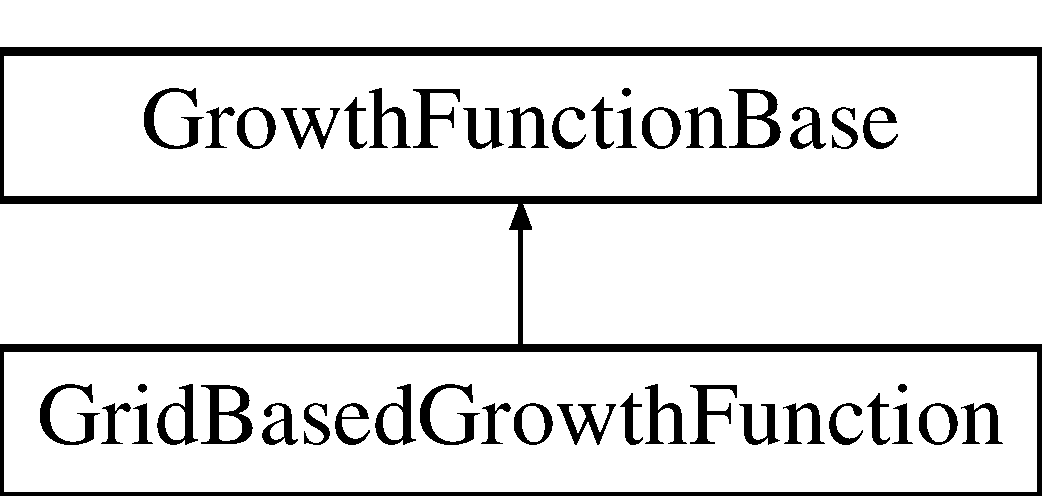
\includegraphics[height=2.000000cm]{classGridBasedGrowthFunction}
\end{center}
\end{figure}
\subsection*{Public Member Functions}
\begin{DoxyCompactItemize}
\item 
\hyperlink{classGridBasedGrowthFunction_aed515e78b2dbcf81751b44cb0c2bef58}{Grid\+Based\+Growth\+Function} (int id, int type, float \hyperlink{classGrowthFunctionBase_ae92513a7b41637df8e26e7db35ddf97c}{init\+Time}, float \hyperlink{classGrowthFunctionBase_a3ff4db0573d354a75666a5f3ca446941}{end\+Time}, bool \hyperlink{classGrowthFunctionBase_a3d56771e7c145589a14e11cc331e0326}{apply\+To\+Columnar\+Layer}, bool \hyperlink{classGrowthFunctionBase_a08ae19f58cb98fa8e315a77f52749732}{apply\+To\+Peripodial\+Membrane}, bool \hyperlink{classGrowthFunctionBase_a9fe46fc6dde4041b79204beb48972a09}{apply\+To\+Basal\+E\+C\+M}, bool \hyperlink{classGrowthFunctionBase_ac623b1dbe376bce5dddbe1a2e21c776f}{apply\+To\+Lateral\+E\+C\+M}, int n\+X, int n\+Y, double $\ast$$\ast$$\ast$Growth\+Mat, double $\ast$$\ast$Angle\+Mat)
\begin{DoxyCompactList}\small\item\em The constructor of \hyperlink{classGridBasedGrowthFunction}{Grid\+Based\+Growth\+Function}. \end{DoxyCompactList}\item 
\hypertarget{classGridBasedGrowthFunction_ae36e6ea2e7bdf41459e74d5846d6d24d}{}int \hyperlink{classGridBasedGrowthFunction_ae36e6ea2e7bdf41459e74d5846d6d24d}{get\+Grid\+X} ()\label{classGridBasedGrowthFunction_ae36e6ea2e7bdf41459e74d5846d6d24d}

\begin{DoxyCompactList}\small\item\em This function returns \hyperlink{classGridBasedGrowthFunction_af872b9963f3a579dcd615c23bcb58a86}{Grid\+Based\+Growth\+Function\+::n\+Grid\+X}. \end{DoxyCompactList}\item 
\hypertarget{classGridBasedGrowthFunction_a4a70e9e187e3079e29115f106d30e26e}{}int \hyperlink{classGridBasedGrowthFunction_a4a70e9e187e3079e29115f106d30e26e}{get\+Grid\+Y} ()\label{classGridBasedGrowthFunction_a4a70e9e187e3079e29115f106d30e26e}

\begin{DoxyCompactList}\small\item\em This function returns \hyperlink{classGridBasedGrowthFunction_a625bc963a1f1e7d1f1a35dbd0ef51728}{Grid\+Based\+Growth\+Function\+::n\+Grid\+Y}. \end{DoxyCompactList}\item 
\hypertarget{classGridBasedGrowthFunction_ac25ac1f12b74816a1d3d3e5dda0e8541}{}double $\ast$$\ast$$\ast$ \hyperlink{classGridBasedGrowthFunction_ac25ac1f12b74816a1d3d3e5dda0e8541}{get\+Growth\+Matrix} ()\label{classGridBasedGrowthFunction_ac25ac1f12b74816a1d3d3e5dda0e8541}

\begin{DoxyCompactList}\small\item\em This function returns \hyperlink{classGridBasedGrowthFunction_a5522d9b84fa95ebd65cdf290a4f0a65c}{Grid\+Based\+Growth\+Function\+::\+Growth\+Matrix}. \end{DoxyCompactList}\item 
\hypertarget{classGridBasedGrowthFunction_ad590b4a5c6e5e47f5679de5a8c6cb738}{}double $\ast$$\ast$ \hyperlink{classGridBasedGrowthFunction_ad590b4a5c6e5e47f5679de5a8c6cb738}{get\+Xy\+Shear\+Angle\+Matrix} ()\label{classGridBasedGrowthFunction_ad590b4a5c6e5e47f5679de5a8c6cb738}

\begin{DoxyCompactList}\small\item\em This function returns \hyperlink{classGridBasedGrowthFunction_aa01cee8282299e18f27b47645da17438}{Grid\+Based\+Growth\+Function\+::xy\+Shear\+Angle\+Matrix}. \end{DoxyCompactList}\item 
\hypertarget{classGridBasedGrowthFunction_a1775fe1788bc97569c892d01cc625ea8}{}double \hyperlink{classGridBasedGrowthFunction_a1775fe1788bc97569c892d01cc625ea8}{get\+Growth\+Matrix\+Element} (int i, int j, int k)\label{classGridBasedGrowthFunction_a1775fe1788bc97569c892d01cc625ea8}

\begin{DoxyCompactList}\small\item\em This function returns the growth rate at grid point \mbox{[}i\mbox{]}\mbox{[}j\mbox{]} (in dimensions \hyperlink{classGridBasedGrowthFunction_af872b9963f3a579dcd615c23bcb58a86}{Grid\+Based\+Growth\+Function\+::n\+Grid\+X}, \hyperlink{classGridBasedGrowthFunction_a625bc963a1f1e7d1f1a35dbd0ef51728}{Grid\+Based\+Growth\+Function\+::n\+Grid\+Y}), for the growth dimension \mbox{[}k\mbox{]} (as in \mbox{[} D\+V axis (x), A\+P axis (y), and A\+B axis (z)\mbox{]} ). \end{DoxyCompactList}\item 
\hypertarget{classGridBasedGrowthFunction_a5075a53329b3a0b73a5864b7ffb37c5d}{}double \hyperlink{classGridBasedGrowthFunction_a5075a53329b3a0b73a5864b7ffb37c5d}{get\+Xy\+Shear\+Angle\+Matrix\+Element} (int i, int j)\label{classGridBasedGrowthFunction_a5075a53329b3a0b73a5864b7ffb37c5d}

\begin{DoxyCompactList}\small\item\em This function returns the xy\+Shear angle at grid point \mbox{[}i\mbox{]}\mbox{[}j\mbox{]} (in dimensions \hyperlink{classGridBasedGrowthFunction_af872b9963f3a579dcd615c23bcb58a86}{Grid\+Based\+Growth\+Function\+::n\+Grid\+X}, \hyperlink{classGridBasedGrowthFunction_a625bc963a1f1e7d1f1a35dbd0ef51728}{Grid\+Based\+Growth\+Function\+::n\+Grid\+Y}). \end{DoxyCompactList}\item 
\hypertarget{classGridBasedGrowthFunction_a85ed4f6a4b5165adf1ab8806b885f81a}{}gsl\+\_\+matrix $\ast$ \hyperlink{classGridBasedGrowthFunction_a85ed4f6a4b5165adf1ab8806b885f81a}{get\+Xy\+Shear\+Rotations\+Matrix\+Element} (int i, int j)\label{classGridBasedGrowthFunction_a85ed4f6a4b5165adf1ab8806b885f81a}

\begin{DoxyCompactList}\small\item\em This function returns the xy\+Shear rotation matrix at grid point \mbox{[}i\mbox{]}\mbox{[}j\mbox{]} (in dimensions \hyperlink{classGridBasedGrowthFunction_af872b9963f3a579dcd615c23bcb58a86}{Grid\+Based\+Growth\+Function\+::n\+Grid\+X}, \hyperlink{classGridBasedGrowthFunction_a625bc963a1f1e7d1f1a35dbd0ef51728}{Grid\+Based\+Growth\+Function\+::n\+Grid\+Y}). \end{DoxyCompactList}\item 
\hypertarget{classGridBasedGrowthFunction_ab07937a18f72f31f4875225c1e246032}{}bool {\bfseries is\+Aspect\+Ratio\+Over\+One} (int i, int j)\label{classGridBasedGrowthFunction_ab07937a18f72f31f4875225c1e246032}

\item 
\hypertarget{classGridBasedGrowthFunction_a9d01fcbba5732aad966659d4f64c145b}{}void \hyperlink{classGridBasedGrowthFunction_a9d01fcbba5732aad966659d4f64c145b}{set\+Growth\+Matrix\+Element} (double ex, double ey, double ez, int i, int j)\label{classGridBasedGrowthFunction_a9d01fcbba5732aad966659d4f64c145b}

\begin{DoxyCompactList}\small\item\em This function sets the growth rate at grid point \mbox{[}i\mbox{]}\mbox{[}j\mbox{]} (in dimensions \hyperlink{classGridBasedGrowthFunction_af872b9963f3a579dcd615c23bcb58a86}{Grid\+Based\+Growth\+Function\+::n\+Grid\+X}, \hyperlink{classGridBasedGrowthFunction_a625bc963a1f1e7d1f1a35dbd0ef51728}{Grid\+Based\+Growth\+Function\+::n\+Grid\+Y}), to the growth rate \mbox{[}ex, ey, ez\mbox{]} in the format \mbox{[} D\+V axis (x), A\+P axis (y), and A\+B axis (z)\mbox{]}. \end{DoxyCompactList}\item 
\hypertarget{classGridBasedGrowthFunction_a92f4db6ab17ba3539f98895c500ec2d7}{}void {\bfseries pre\+Calculate\+Angles\+For\+Compatible\+Averaging} ()\label{classGridBasedGrowthFunction_a92f4db6ab17ba3539f98895c500ec2d7}

\item 
\hypertarget{classGridBasedGrowthFunction_a11692e47b20e812fe775f99a78480571}{}void {\bfseries get\+Growth\+Profile\+At4\+Corners} (int Index\+X, int Index\+Y, double $\ast$growth0, double $\ast$growth1, double $\ast$growth2, double $\ast$growth3, double $\ast$angles, bool $\ast$angles\+Eliminated)\label{classGridBasedGrowthFunction_a11692e47b20e812fe775f99a78480571}

\item 
void \hyperlink{classGridBasedGrowthFunction_a267f45c300d9ef98c6f4fa14a5181c78}{write\+Summary} (ofstream \&save\+File\+Simulation\+Summary)
\begin{DoxyCompactList}\small\item\em The function is to write the growth function summary to simulation summary file. \end{DoxyCompactList}\end{DoxyCompactItemize}
\subsection*{Public Attributes}
\begin{DoxyCompactItemize}
\item 
\hypertarget{classGridBasedGrowthFunction_af872b9963f3a579dcd615c23bcb58a86}{}int \hyperlink{classGridBasedGrowthFunction_af872b9963f3a579dcd615c23bcb58a86}{n\+Grid\+X}\label{classGridBasedGrowthFunction_af872b9963f3a579dcd615c23bcb58a86}

\begin{DoxyCompactList}\small\item\em The number of grid points that discretise the tissue in x. \end{DoxyCompactList}\item 
\hypertarget{classGridBasedGrowthFunction_a625bc963a1f1e7d1f1a35dbd0ef51728}{}int \hyperlink{classGridBasedGrowthFunction_a625bc963a1f1e7d1f1a35dbd0ef51728}{n\+Grid\+Y}\label{classGridBasedGrowthFunction_a625bc963a1f1e7d1f1a35dbd0ef51728}

\begin{DoxyCompactList}\small\item\em The number of grid points that discretise the tissue in y. \end{DoxyCompactList}\item 
\hypertarget{classGridBasedGrowthFunction_a5522d9b84fa95ebd65cdf290a4f0a65c}{}double $\ast$$\ast$$\ast$ \hyperlink{classGridBasedGrowthFunction_a5522d9b84fa95ebd65cdf290a4f0a65c}{Growth\+Matrix}\label{classGridBasedGrowthFunction_a5522d9b84fa95ebd65cdf290a4f0a65c}

\begin{DoxyCompactList}\small\item\em The matrix of growth rates in (1/sec). It is a matrix of double triplets for growth rate at each grid point. The dimensions of the matrix are equal to (\hyperlink{classGridBasedGrowthFunction_af872b9963f3a579dcd615c23bcb58a86}{Grid\+Based\+Growth\+Function\+::n\+Grid\+X}, \hyperlink{classGridBasedGrowthFunction_a625bc963a1f1e7d1f1a35dbd0ef51728}{Grid\+Based\+Growth\+Function\+::n\+Grid\+Y}), and set in constructor of the \hyperlink{classGridBasedGrowthFunction}{Grid\+Based\+Growth\+Function}. The triplets store the growth rate in \mbox{[} D\+V axis (x), A\+P axis (y), and A\+B axis (z)\mbox{]}. \end{DoxyCompactList}\item 
\hypertarget{classGridBasedGrowthFunction_aa01cee8282299e18f27b47645da17438}{}double $\ast$$\ast$ \hyperlink{classGridBasedGrowthFunction_aa01cee8282299e18f27b47645da17438}{xy\+Shear\+Angle\+Matrix}\label{classGridBasedGrowthFunction_aa01cee8282299e18f27b47645da17438}

\begin{DoxyCompactList}\small\item\em The matrix of xy shear rate (rad/sec). It is a matrix of doubles at each grid point. he dimensions of the matrix are equal to (\hyperlink{classGridBasedGrowthFunction_af872b9963f3a579dcd615c23bcb58a86}{Grid\+Based\+Growth\+Function\+::n\+Grid\+X}, \hyperlink{classGridBasedGrowthFunction_a625bc963a1f1e7d1f1a35dbd0ef51728}{Grid\+Based\+Growth\+Function\+::n\+Grid\+Y}), and set in constructor of the \hyperlink{classGridBasedGrowthFunction}{Grid\+Based\+Growth\+Function}. \end{DoxyCompactList}\item 
\hypertarget{classGridBasedGrowthFunction_a62e3267b367261ff2f37cee9a7c2b02b}{}gsl\+\_\+matrix $\ast$$\ast$$\ast$ {\bfseries xy\+Shear\+Rotations\+Matrix}\label{classGridBasedGrowthFunction_a62e3267b367261ff2f37cee9a7c2b02b}

\item 
\hypertarget{classGridBasedGrowthFunction_a56ff4380487e4d24881431f0e6ea6f2e}{}bool $\ast$$\ast$ {\bfseries aspect\+Ratio\+Over\+Thresold\+Matrix}\label{classGridBasedGrowthFunction_a56ff4380487e4d24881431f0e6ea6f2e}

\item 
\hypertarget{classGridBasedGrowthFunction_a59b0e127387157f89f099ae3beeaa671}{}double $\ast$$\ast$$\ast$$\ast$ {\bfseries compatible\+Growths}\label{classGridBasedGrowthFunction_a59b0e127387157f89f099ae3beeaa671}

\item 
\hypertarget{classGridBasedGrowthFunction_aac8a163bbd008d327859b488cf023c10}{}double $\ast$$\ast$$\ast$ {\bfseries compatible\+Angles}\label{classGridBasedGrowthFunction_aac8a163bbd008d327859b488cf023c10}

\item 
\hypertarget{classGridBasedGrowthFunction_addfc2d280d1fc0b0b17d7f1dfe54f873}{}bool $\ast$$\ast$$\ast$ {\bfseries compatible\+Angle\+Eliminated}\label{classGridBasedGrowthFunction_addfc2d280d1fc0b0b17d7f1dfe54f873}

\end{DoxyCompactItemize}


\subsection{Constructor \& Destructor Documentation}
\hypertarget{classGridBasedGrowthFunction_aed515e78b2dbcf81751b44cb0c2bef58}{}\index{Grid\+Based\+Growth\+Function@{Grid\+Based\+Growth\+Function}!Grid\+Based\+Growth\+Function@{Grid\+Based\+Growth\+Function}}
\index{Grid\+Based\+Growth\+Function@{Grid\+Based\+Growth\+Function}!Grid\+Based\+Growth\+Function@{Grid\+Based\+Growth\+Function}}
\subsubsection[{Grid\+Based\+Growth\+Function}]{\setlength{\rightskip}{0pt plus 5cm}Grid\+Based\+Growth\+Function\+::\+Grid\+Based\+Growth\+Function (
\begin{DoxyParamCaption}
\item[{int}]{id, }
\item[{int}]{type, }
\item[{float}]{init\+Time, }
\item[{float}]{end\+Time, }
\item[{bool}]{apply\+To\+Columnar\+Layer, }
\item[{bool}]{apply\+To\+Peripodial\+Membrane, }
\item[{bool}]{apply\+To\+Basal\+E\+C\+M, }
\item[{bool}]{apply\+To\+Lateral\+E\+C\+M, }
\item[{int}]{n\+X, }
\item[{int}]{n\+Y, }
\item[{double $\ast$$\ast$$\ast$}]{Growth\+Mat, }
\item[{double $\ast$$\ast$}]{Angle\+Mat}
\end{DoxyParamCaption}
)\hspace{0.3cm}{\ttfamily [inline]}}\label{classGridBasedGrowthFunction_aed515e78b2dbcf81751b44cb0c2bef58}


The constructor of \hyperlink{classGridBasedGrowthFunction}{Grid\+Based\+Growth\+Function}. 

The first six parameters will be directed to the parent constructor, \hyperlink{classGrowthFunctionBase_a5c275b3f839cc4f572b68afc5ad1064f}{Growth\+Function\+Base\+::\+Growth\+Function\+Base}. ~\newline
integers n\+X and n\+Y will set \hyperlink{classGridBasedGrowthFunction_af872b9963f3a579dcd615c23bcb58a86}{Grid\+Based\+Growth\+Function\+::n\+Grid\+X} and \hyperlink{classGridBasedGrowthFunction_a625bc963a1f1e7d1f1a35dbd0ef51728}{Grid\+Based\+Growth\+Function\+::n\+Grid\+Y}, respectively. \hyperlink{classGridBasedGrowthFunction_a5522d9b84fa95ebd65cdf290a4f0a65c}{Grid\+Based\+Growth\+Function\+::\+Growth\+Matrix} will be initiated to point at a 2 dimensional matrix of double triplets the size(n\+X, n\+Y). ~\newline
double$\ast$$\ast$$\ast$ Growth\+Mat is the pointer to the 2-\/dimensional matrix of double triplets, holding the 3\+D growth rates at each grid point. Values stored in Growth\+Mat will set the values in \hyperlink{classGridBasedGrowthFunction_a5522d9b84fa95ebd65cdf290a4f0a65c}{Grid\+Based\+Growth\+Function\+::\+Growth\+Matrix}. The matrix storing the growth rates have been read from an input file through Model\+Input\+Object\+::read\+Growth\+Options and related functions therein ~\newline
 

\subsection{Member Function Documentation}
\hypertarget{classGridBasedGrowthFunction_a267f45c300d9ef98c6f4fa14a5181c78}{}\index{Grid\+Based\+Growth\+Function@{Grid\+Based\+Growth\+Function}!write\+Summary@{write\+Summary}}
\index{write\+Summary@{write\+Summary}!Grid\+Based\+Growth\+Function@{Grid\+Based\+Growth\+Function}}
\subsubsection[{write\+Summary}]{\setlength{\rightskip}{0pt plus 5cm}void Grid\+Based\+Growth\+Function\+::write\+Summary (
\begin{DoxyParamCaption}
\item[{ofstream \&}]{save\+File\+Simulation\+Summary}
\end{DoxyParamCaption}
)\hspace{0.3cm}{\ttfamily [inline]}, {\ttfamily [virtual]}}\label{classGridBasedGrowthFunction_a267f45c300d9ef98c6f4fa14a5181c78}


The function is to write the growth function summary to simulation summary file. 

This function will write the \hyperlink{classGridBasedGrowthFunction}{Grid\+Based\+Growth\+Function} details into the simulation summary file, provided as the first input. The output should look like\+: ~\newline
 Growth Type\+: growth From File (3) Initial time(sec)\+: \hyperlink{classGrowthFunctionBase_ae92513a7b41637df8e26e7db35ddf97c}{Grid\+Based\+Growth\+Function\+::init\+Time} Final\+Time time(sec)\+: \hyperlink{classGrowthFunctionBase_a3ff4db0573d354a75666a5f3ca446941}{Grid\+Based\+Growth\+Function\+::end\+Time} Growth matrix mesh size\+: \hyperlink{classGridBasedGrowthFunction_af872b9963f3a579dcd615c23bcb58a86}{Grid\+Based\+Growth\+Function\+::n\+Grid\+X} \hyperlink{classGridBasedGrowthFunction_a625bc963a1f1e7d1f1a35dbd0ef51728}{Grid\+Based\+Growth\+Function\+::n\+Grid\+Y}

Reimplemented from \hyperlink{classGrowthFunctionBase}{Growth\+Function\+Base}.



The documentation for this class was generated from the following file\+:\begin{DoxyCompactItemize}
\item 
/home/melda/\+Documents/\+Tissue\+Folding/\+Tissue\+Folding/\+Source\+Code/Growth\+Function\+Types.\+h\end{DoxyCompactItemize}

\hypertarget{classGrowthFunctionBase}{}\section{Growth\+Function\+Base Class Reference}
\label{classGrowthFunctionBase}\index{Growth\+Function\+Base@{Growth\+Function\+Base}}
Inheritance diagram for Growth\+Function\+Base\+:\begin{figure}[H]
\begin{center}
\leavevmode
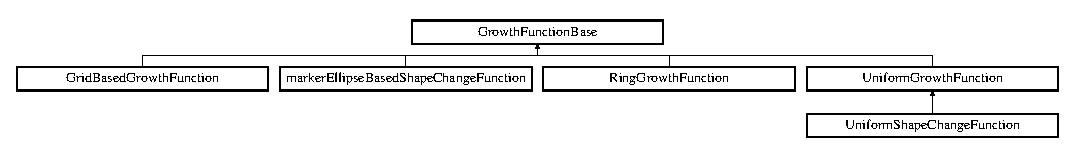
\includegraphics[height=2.916667cm]{classGrowthFunctionBase}
\end{center}
\end{figure}
\subsection*{Public Member Functions}
\begin{DoxyCompactItemize}
\item 
\hyperlink{classGrowthFunctionBase_a061b31ad8a0cb228628c7104029a94bf}{Growth\+Function\+Base} (int id, int type, float \hyperlink{classGrowthFunctionBase_ae92513a7b41637df8e26e7db35ddf97c}{init\+Time}, float \hyperlink{classGrowthFunctionBase_a3ff4db0573d354a75666a5f3ca446941}{end\+Time}, bool \hyperlink{classGrowthFunctionBase_a3d56771e7c145589a14e11cc331e0326}{apply\+To\+Columnar\+Layer}, bool \hyperlink{classGrowthFunctionBase_a08ae19f58cb98fa8e315a77f52749732}{apply\+To\+Peripodial\+Membrane})
\begin{DoxyCompactList}\small\item\em The constructor of \hyperlink{classGrowthFunctionBase}{Growth\+Function\+Base}. Different growth functions will be derived from this class. \end{DoxyCompactList}\item 
\hypertarget{classGrowthFunctionBase_ad5b4e88d33c4b72444c5c25c25ab68fb}{}void {\bfseries Parent\+Error\+Message} (string function\+Name)\label{classGrowthFunctionBase_ad5b4e88d33c4b72444c5c25c25ab68fb}

\item 
\hypertarget{classGrowthFunctionBase_aed234af9feb797628d4a2d598dcf9632}{}double {\bfseries Parent\+Error\+Message} (string function\+Name, double return\+Value)\label{classGrowthFunctionBase_aed234af9feb797628d4a2d598dcf9632}

\item 
\hypertarget{classGrowthFunctionBase_a9097ca54f854aa0d1c8d220c971580dd}{}int {\bfseries Parent\+Error\+Message} (string function\+Name, int return\+Value)\label{classGrowthFunctionBase_a9097ca54f854aa0d1c8d220c971580dd}

\item 
\hypertarget{classGrowthFunctionBase_abd31142fe0bcc9a95a39c85cb55438a8}{}virtual void {\bfseries write\+Summary} (ofstream \&save\+File\+Simulation\+Summary, double dt)\label{classGrowthFunctionBase_abd31142fe0bcc9a95a39c85cb55438a8}

\item 
\hypertarget{classGrowthFunctionBase_aa031bd3d28993402ee5bdb3d8cae7fa6}{}virtual void {\bfseries get\+Centre} (float \&centre\+X, float \&centre\+Y)\label{classGrowthFunctionBase_aa031bd3d28993402ee5bdb3d8cae7fa6}

\item 
\hypertarget{classGrowthFunctionBase_a05ace7e6cb21566ad03e72e56962d58b}{}virtual float {\bfseries get\+Inner\+Radius} ()\label{classGrowthFunctionBase_a05ace7e6cb21566ad03e72e56962d58b}

\item 
\hypertarget{classGrowthFunctionBase_a2ba8f7659e1c0546998671458943233d}{}virtual float {\bfseries get\+Outer\+Radius} ()\label{classGrowthFunctionBase_a2ba8f7659e1c0546998671458943233d}

\item 
\hypertarget{classGrowthFunctionBase_a9598654cae114f6b443167898ac4d095}{}virtual void {\bfseries get\+Growth\+Rate} (double $\ast$max\+Value)\label{classGrowthFunctionBase_a9598654cae114f6b443167898ac4d095}

\item 
\hypertarget{classGrowthFunctionBase_a3c0d71849d020d29832b1aaaba87065e}{}virtual gsl\+\_\+matrix $\ast$ {\bfseries get\+Shear\+Angle\+Rotation\+Matrix} ()\label{classGrowthFunctionBase_a3c0d71849d020d29832b1aaaba87065e}

\item 
\hypertarget{classGrowthFunctionBase_adea116613ddb2edb7ebc0734d17c9226}{}virtual double {\bfseries get\+Shear\+Angle} ()\label{classGrowthFunctionBase_adea116613ddb2edb7ebc0734d17c9226}

\item 
\hypertarget{classGrowthFunctionBase_a1dfd024db9bf627777741c68f7b5ddf2}{}virtual int {\bfseries get\+Grid\+X} ()\label{classGrowthFunctionBase_a1dfd024db9bf627777741c68f7b5ddf2}

\item 
\hypertarget{classGrowthFunctionBase_a1445bfc812abb72fd6757859aa302feb}{}virtual int {\bfseries get\+Grid\+Y} ()\label{classGrowthFunctionBase_a1445bfc812abb72fd6757859aa302feb}

\item 
\hypertarget{classGrowthFunctionBase_a067bdcd836e7196ce5cfc9120b9499c1}{}virtual double $\ast$$\ast$$\ast$ {\bfseries get\+Growth\+Matrix} ()\label{classGrowthFunctionBase_a067bdcd836e7196ce5cfc9120b9499c1}

\item 
\hypertarget{classGrowthFunctionBase_a32e0a776bc81147dc648662440d50b0d}{}virtual double $\ast$$\ast$ {\bfseries get\+Xy\+Shear\+Angle\+Matrix} ()\label{classGrowthFunctionBase_a32e0a776bc81147dc648662440d50b0d}

\item 
\hypertarget{classGrowthFunctionBase_a4e40d019aff99e72b1aee79d93c8e9a0}{}virtual double {\bfseries get\+Growth\+Matrix\+Element} (int i, int j, int k)\label{classGrowthFunctionBase_a4e40d019aff99e72b1aee79d93c8e9a0}

\item 
\hypertarget{classGrowthFunctionBase_adfa5e38c1b2d748c035a3bdbe8717d73}{}virtual double {\bfseries get\+Xy\+Shear\+Angle\+Matrix\+Element} (int i, int j)\label{classGrowthFunctionBase_adfa5e38c1b2d748c035a3bdbe8717d73}

\item 
\hypertarget{classGrowthFunctionBase_a01bd724756ffac9b8c1d1693b2547588}{}virtual bool {\bfseries is\+Aspect\+Ratio\+Over\+One} (int i, int j)\label{classGrowthFunctionBase_a01bd724756ffac9b8c1d1693b2547588}

\item 
\hypertarget{classGrowthFunctionBase_a70f43b1e57d2be8ca0e2a937da333dfa}{}virtual gsl\+\_\+matrix $\ast$ {\bfseries get\+Xy\+Shear\+Rotations\+Matrix\+Element} (int i, int j)\label{classGrowthFunctionBase_a70f43b1e57d2be8ca0e2a937da333dfa}

\item 
\hypertarget{classGrowthFunctionBase_ae529d0ae06ca241d94bfa8fd831af99b}{}virtual void {\bfseries get\+Growth\+Profile\+At4\+Corners} (int Index\+X, int Index\+Y, double $\ast$growth0, double $\ast$growth1, double $\ast$growth2, double $\ast$growth3, double $\ast$angles, bool $\ast$angles\+Eliminated)\label{classGrowthFunctionBase_ae529d0ae06ca241d94bfa8fd831af99b}

\item 
\hypertarget{classGrowthFunctionBase_abcfbd2e1fbad91b3f9002ef7fc7625e5}{}virtual void {\bfseries set\+Growt\+Rate} (double ex, double ey, double ez)\label{classGrowthFunctionBase_abcfbd2e1fbad91b3f9002ef7fc7625e5}

\item 
\hypertarget{classGrowthFunctionBase_a29781080624a8ab028af36f3326b6240}{}virtual void {\bfseries set\+Growth\+Matrix\+Element} (double ex, double ey, double ez, int i, int j)\label{classGrowthFunctionBase_a29781080624a8ab028af36f3326b6240}

\end{DoxyCompactItemize}
\subsection*{Public Attributes}
\begin{DoxyCompactItemize}
\item 
\hypertarget{classGrowthFunctionBase_a90fc4b14e2adcda0930fe93b1490fb7a}{}int \hyperlink{classGrowthFunctionBase_a90fc4b14e2adcda0930fe93b1490fb7a}{Type}\label{classGrowthFunctionBase_a90fc4b14e2adcda0930fe93b1490fb7a}

\begin{DoxyCompactList}\small\item\em The type of the growth function, 1\+: uniform growth, 2\+: Ring shaped growth, 3\+: Grid based growth, where growth rates read from a separate input file. \end{DoxyCompactList}\item 
\hypertarget{classGrowthFunctionBase_aa669a940ab77009f9b2b9c9885e9cd9e}{}int \hyperlink{classGrowthFunctionBase_aa669a940ab77009f9b2b9c9885e9cd9e}{Id}\label{classGrowthFunctionBase_aa669a940ab77009f9b2b9c9885e9cd9e}

\begin{DoxyCompactList}\small\item\em The unique identification number of the growth function. \end{DoxyCompactList}\item 
\hypertarget{classGrowthFunctionBase_ae92513a7b41637df8e26e7db35ddf97c}{}float \hyperlink{classGrowthFunctionBase_ae92513a7b41637df8e26e7db35ddf97c}{init\+Time}\label{classGrowthFunctionBase_ae92513a7b41637df8e26e7db35ddf97c}

\begin{DoxyCompactList}\small\item\em The initiation time of the growth, in seconds. \end{DoxyCompactList}\item 
\hypertarget{classGrowthFunctionBase_a3ff4db0573d354a75666a5f3ca446941}{}float \hyperlink{classGrowthFunctionBase_a3ff4db0573d354a75666a5f3ca446941}{end\+Time}\label{classGrowthFunctionBase_a3ff4db0573d354a75666a5f3ca446941}

\begin{DoxyCompactList}\small\item\em The end time of the growth, in seconds. \end{DoxyCompactList}\item 
\hypertarget{classGrowthFunctionBase_a3d56771e7c145589a14e11cc331e0326}{}bool \hyperlink{classGrowthFunctionBase_a3d56771e7c145589a14e11cc331e0326}{apply\+To\+Columnar\+Layer}\label{classGrowthFunctionBase_a3d56771e7c145589a14e11cc331e0326}

\begin{DoxyCompactList}\small\item\em Boolean stating if the growth should be applied to columnar layer. \end{DoxyCompactList}\item 
\hypertarget{classGrowthFunctionBase_a08ae19f58cb98fa8e315a77f52749732}{}bool \hyperlink{classGrowthFunctionBase_a08ae19f58cb98fa8e315a77f52749732}{apply\+To\+Peripodial\+Membrane}\label{classGrowthFunctionBase_a08ae19f58cb98fa8e315a77f52749732}

\begin{DoxyCompactList}\small\item\em Boolean stating if the growth should be applied to peripodial membrane. \end{DoxyCompactList}\end{DoxyCompactItemize}


\subsection{Constructor \& Destructor Documentation}
\hypertarget{classGrowthFunctionBase_a061b31ad8a0cb228628c7104029a94bf}{}\index{Growth\+Function\+Base@{Growth\+Function\+Base}!Growth\+Function\+Base@{Growth\+Function\+Base}}
\index{Growth\+Function\+Base@{Growth\+Function\+Base}!Growth\+Function\+Base@{Growth\+Function\+Base}}
\subsubsection[{Growth\+Function\+Base}]{\setlength{\rightskip}{0pt plus 5cm}Growth\+Function\+Base\+::\+Growth\+Function\+Base (
\begin{DoxyParamCaption}
\item[{int}]{id, }
\item[{int}]{type, }
\item[{float}]{init\+Time, }
\item[{float}]{end\+Time, }
\item[{bool}]{apply\+To\+Columnar\+Layer, }
\item[{bool}]{apply\+To\+Peripodial\+Membrane}
\end{DoxyParamCaption}
)\hspace{0.3cm}{\ttfamily [inline]}}\label{classGrowthFunctionBase_a061b31ad8a0cb228628c7104029a94bf}


The constructor of \hyperlink{classGrowthFunctionBase}{Growth\+Function\+Base}. Different growth functions will be derived from this class. 

integer id will set \hyperlink{classGrowthFunctionBase_aa669a940ab77009f9b2b9c9885e9cd9e}{Growth\+Function\+Base\+::\+Id}. ~\newline
integer type will set \hyperlink{classGrowthFunctionBase_a90fc4b14e2adcda0930fe93b1490fb7a}{Growth\+Function\+Base\+::\+Type}. ~\newline
floats init\+Time and end\+Time will set \hyperlink{classGrowthFunctionBase_ae92513a7b41637df8e26e7db35ddf97c}{Growth\+Function\+Base\+::init\+Time} and \hyperlink{classGrowthFunctionBase_a3ff4db0573d354a75666a5f3ca446941}{Growth\+Function\+Base\+::end\+Time} respectively. ~\newline
booleans apply\+To\+Columnar\+Layer and apply\+To\+Peripodial\+Membrane will set \hyperlink{classGrowthFunctionBase_a3d56771e7c145589a14e11cc331e0326}{Growth\+Function\+Base\+::apply\+To\+Columnar\+Layer} and \hyperlink{classGrowthFunctionBase_a08ae19f58cb98fa8e315a77f52749732}{Growth\+Function\+Base\+::apply\+To\+Peripodial\+Membrane}, respectively. ~\newline
 

The documentation for this class was generated from the following file\+:\begin{DoxyCompactItemize}
\item 
/home/melda/\+Documents/\+Tissue\+Folding/\+Tissue\+Folding/\+Source\+Code/Growth\+Function\+Base.\+h\end{DoxyCompactItemize}

\hypertarget{classMainWindow}{}\section{Main\+Window Class Reference}
\label{classMainWindow}\index{Main\+Window@{Main\+Window}}
Inheritance diagram for Main\+Window\+:\begin{figure}[H]
\begin{center}
\leavevmode
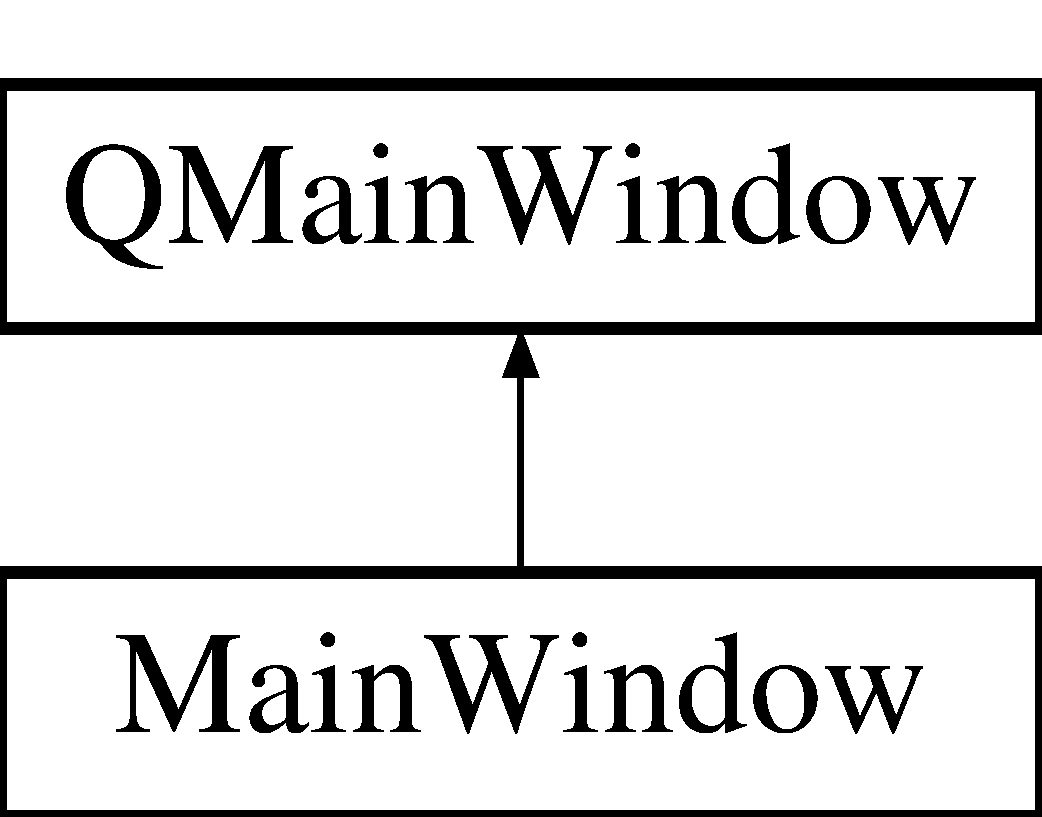
\includegraphics[height=2.000000cm]{classMainWindow}
\end{center}
\end{figure}
\subsection*{Public Slots}
\begin{DoxyCompactItemize}
\item 
\hypertarget{classMainWindow_ab2c0d4d0d84826cc032a45ea4783dde5}{}void {\bfseries Selected\+Item\+Change} ()\label{classMainWindow_ab2c0d4d0d84826cc032a45ea4783dde5}

\item 
\hypertarget{classMainWindow_a99f4fa67c708306ecac0eb351c6968d6}{}void {\bfseries manual\+Node\+Selection} (const Q\+String \&)\label{classMainWindow_a99f4fa67c708306ecac0eb351c6968d6}

\item 
\hypertarget{classMainWindow_af6253ec8c287b675a80e80bdd0ad31cc}{}void {\bfseries manual\+Element\+Selection} (const Q\+String \&)\label{classMainWindow_af6253ec8c287b675a80e80bdd0ad31cc}

\item 
\hypertarget{classMainWindow_ad613f2de4daee9c84828dc0490b00ffa}{}void {\bfseries Manual\+Element\+Selection\+Reset} ()\label{classMainWindow_ad613f2de4daee9c84828dc0490b00ffa}

\item 
\hypertarget{classMainWindow_a52630b918235794e8ff6cfd6abfc4b7f}{}void {\bfseries Manual\+Node\+Selection\+Reset} ()\label{classMainWindow_a52630b918235794e8ff6cfd6abfc4b7f}

\item 
\hypertarget{classMainWindow_a59dd1f2fe0d6900a98feff45c94e23e6}{}void {\bfseries timer\+Simulation\+Step} ()\label{classMainWindow_a59dd1f2fe0d6900a98feff45c94e23e6}

\item 
\hypertarget{classMainWindow_a0dce0c101c73abe3b5f347cd4dacfbd3}{}void {\bfseries update\+Strain} (int)\label{classMainWindow_a0dce0c101c73abe3b5f347cd4dacfbd3}

\item 
\hypertarget{classMainWindow_a99a35d2b2c33a4cadab365403816c15c}{}void {\bfseries update\+Strain\+Check\+Box} (int)\label{classMainWindow_a99a35d2b2c33a4cadab365403816c15c}

\item 
\hypertarget{classMainWindow_a18d28bd55cc52f4b81d1c09e655d9711}{}void {\bfseries update\+Strain\+Spin\+Boxes} (double)\label{classMainWindow_a18d28bd55cc52f4b81d1c09e655d9711}

\item 
\hypertarget{classMainWindow_a524bf8d075a209be107c5ee9cd750bba}{}void {\bfseries update\+Pys\+Prop} (int s)\label{classMainWindow_a524bf8d075a209be107c5ee9cd750bba}

\item 
\hypertarget{classMainWindow_a933538d0ccf6de1298c6e4c7ed223f38}{}void {\bfseries update\+Pys\+Check\+Box} (int)\label{classMainWindow_a933538d0ccf6de1298c6e4c7ed223f38}

\item 
\hypertarget{classMainWindow_acd6a8996cd12c70a0e0572eebb9dc24d}{}void {\bfseries update\+Pys\+Prop\+Spin\+Boxes} (double d)\label{classMainWindow_acd6a8996cd12c70a0e0572eebb9dc24d}

\item 
\hypertarget{classMainWindow_ad30193e1dac5d64c7467e576e238ce03}{}void {\bfseries update\+Display\+Pipette} (int)\label{classMainWindow_ad30193e1dac5d64c7467e576e238ce03}

\item 
\hypertarget{classMainWindow_ac6e570780295db3ff54382cbda1ea4cf}{}void {\bfseries update\+Net\+Force\+Check\+Box} (int)\label{classMainWindow_ac6e570780295db3ff54382cbda1ea4cf}

\item 
\hypertarget{classMainWindow_abf1716feb02925cadc40800ed5aa1af8}{}void {\bfseries update\+Packing\+Force\+Check\+Box} (int)\label{classMainWindow_abf1716feb02925cadc40800ed5aa1af8}

\item 
\hypertarget{classMainWindow_a0860bef7bbd9ae81c607142a8462e0a7}{}void {\bfseries update\+Velocity\+Check\+Box} (int)\label{classMainWindow_a0860bef7bbd9ae81c607142a8462e0a7}

\item 
\hypertarget{classMainWindow_af7f60ea4eea7ff11fd1f892455d86063}{}void {\bfseries update\+Scale\+Bar\+Check\+Box} (int)\label{classMainWindow_af7f60ea4eea7ff11fd1f892455d86063}

\item 
\hypertarget{classMainWindow_aee2509de2d13eedd782420cf86cd34d6}{}void {\bfseries update\+Peripodial\+Display\+Check\+Box} (int s)\label{classMainWindow_aee2509de2d13eedd782420cf86cd34d6}

\item 
\hypertarget{classMainWindow_a516111157b177a92fc5838a060f36908}{}void {\bfseries update\+Columnar\+Layer\+Display\+Check\+Box} (int s)\label{classMainWindow_a516111157b177a92fc5838a060f36908}

\item 
\hypertarget{classMainWindow_a52aa21a413bbc1f33a84f695b677f490}{}void {\bfseries update\+Bounding\+Box\+Check\+Box} (int s)\label{classMainWindow_a52aa21a413bbc1f33a84f695b677f490}

\item 
\hypertarget{classMainWindow_af2c325c24155eb2198ef705d78d452d8}{}void {\bfseries update\+Orthagonal\+Perspective\+View\+Toggle} ()\label{classMainWindow_af2c325c24155eb2198ef705d78d452d8}

\item 
\hypertarget{classMainWindow_ab677ef1bf70bc78faa5680576c14cd22}{}void {\bfseries x\+Clip\+Change} (int)\label{classMainWindow_ab677ef1bf70bc78faa5680576c14cd22}

\item 
\hypertarget{classMainWindow_a019023e11d09610ad8632baeb6854c61}{}void {\bfseries y\+Clip\+Change} (int)\label{classMainWindow_a019023e11d09610ad8632baeb6854c61}

\item 
\hypertarget{classMainWindow_af30a90f508a3d0b4434ddcaf848c69ac}{}void {\bfseries z\+Clip\+Change} (int)\label{classMainWindow_af30a90f508a3d0b4434ddcaf848c69ac}

\end{DoxyCompactItemize}
\subsection*{Public Member Functions}
\begin{DoxyCompactItemize}
\item 
\hypertarget{classMainWindow_aa1c3a3a33e1e67e055b8448ad9a9e208}{}{\bfseries Main\+Window} (\hyperlink{classSimulation}{Simulation} $\ast$S\+Im01)\label{classMainWindow_aa1c3a3a33e1e67e055b8448ad9a9e208}

\end{DoxyCompactItemize}
\subsection*{Public Attributes}
\begin{DoxyCompactItemize}
\item 
\hypertarget{classMainWindow_a9604326eab0369c7de6be01f992e0ba7}{}Q\+Graphics\+Scene $\ast$ {\bfseries Main\+Scene}\label{classMainWindow_a9604326eab0369c7de6be01f992e0ba7}

\item 
\hypertarget{classMainWindow_a80b2787fc058a3f5141b905d6c69c0ad}{}Q\+V\+Box\+Layout $\ast$ {\bfseries Control\+Panel\+Main\+H\+Box}\label{classMainWindow_a80b2787fc058a3f5141b905d6c69c0ad}

\item 
\hypertarget{classMainWindow_a028cf99e2842ca1250d4c103310c3430}{}Q\+Grid\+Layout $\ast$ {\bfseries Main\+Grid}\label{classMainWindow_a028cf99e2842ca1250d4c103310c3430}

\item 
\hypertarget{classMainWindow_aebd88a36f5ea16df9a037f7591090856}{}\hyperlink{classGLWidget}{G\+L\+Widget} $\ast$ {\bfseries Main\+G\+L\+Widget}\label{classMainWindow_aebd88a36f5ea16df9a037f7591090856}

\item 
\hypertarget{classMainWindow_aedd252a3fb1c0e6c7fe2d9edb5d19b83}{}\hyperlink{classSimulation}{Simulation} $\ast$ {\bfseries Sim01}\label{classMainWindow_aedd252a3fb1c0e6c7fe2d9edb5d19b83}

\end{DoxyCompactItemize}


The documentation for this class was generated from the following files\+:\begin{DoxyCompactItemize}
\item 
/home/melda/\+Documents/\+Tissue\+Folding/\+User\+Interface/\+Source\+Code/Main\+Window.\+h\item 
/home/melda/\+Documents/\+Tissue\+Folding/\+User\+Interface/\+Source\+Code/Main\+Window.\+cpp\end{DoxyCompactItemize}

\hypertarget{classModelInputObject}{}\section{Model\+Input\+Object Class Reference}
\label{classModelInputObject}\index{Model\+Input\+Object@{Model\+Input\+Object}}


{\ttfamily \#include $<$Model\+Input\+Object.\+h$>$}

\subsection*{Public Member Functions}
\begin{DoxyCompactItemize}
\item 
\hypertarget{classModelInputObject_a64b031469546b19177c0a13365058162}{}\hyperlink{classModelInputObject_a64b031469546b19177c0a13365058162}{Model\+Input\+Object} ()\label{classModelInputObject_a64b031469546b19177c0a13365058162}

\begin{DoxyCompactList}\small\item\em The constructor of the \hyperlink{classModelInputObject}{Model\+Input\+Object}. \end{DoxyCompactList}\item 
bool \hyperlink{classModelInputObject_a9741685527f446bd2bf66455c5b01d0c}{read\+Parameters} ()
\begin{DoxyCompactList}\small\item\em This is the main funciton reading the parameters from file. \end{DoxyCompactList}\end{DoxyCompactItemize}
\subsection*{Public Attributes}
\begin{DoxyCompactItemize}
\item 
\hypertarget{classModelInputObject_a0c5fb50d9d705bc9a9b4fafeebd1cadc}{}\hyperlink{classSimulation}{Simulation} $\ast$ \hyperlink{classModelInputObject_a0c5fb50d9d705bc9a9b4fafeebd1cadc}{Sim}\label{classModelInputObject_a0c5fb50d9d705bc9a9b4fafeebd1cadc}

\begin{DoxyCompactList}\small\item\em The pointer to the simulation object, for which the parameters are being read from the modelinput file. \end{DoxyCompactList}\item 
\hypertarget{classModelInputObject_a32fadb000159d03f6c5901ce3167ada8}{}const char $\ast$ \hyperlink{classModelInputObject_a32fadb000159d03f6c5901ce3167ada8}{parameter\+File\+Name}\label{classModelInputObject_a32fadb000159d03f6c5901ce3167ada8}

\begin{DoxyCompactList}\small\item\em The name (including path) of the file containing the model input parameters. \end{DoxyCompactList}\item 
\hypertarget{classModelInputObject_a2621e76abbd05573aea2d5471a589405}{}string \hyperlink{classModelInputObject_a2621e76abbd05573aea2d5471a589405}{mesh\+File\+Name}\label{classModelInputObject_a2621e76abbd05573aea2d5471a589405}

\begin{DoxyCompactList}\small\item\em The name (including path) of the file containing the input mesh file for tissue geometry. \end{DoxyCompactList}\end{DoxyCompactItemize}


\subsection{Detailed Description}
\hyperlink{classModelInputObject}{Model\+Input\+Object} class 

\subsection{Member Function Documentation}
\hypertarget{classModelInputObject_a9741685527f446bd2bf66455c5b01d0c}{}\index{Model\+Input\+Object@{Model\+Input\+Object}!read\+Parameters@{read\+Parameters}}
\index{read\+Parameters@{read\+Parameters}!Model\+Input\+Object@{Model\+Input\+Object}}
\subsubsection[{read\+Parameters}]{\setlength{\rightskip}{0pt plus 5cm}bool Model\+Input\+Object\+::read\+Parameters (
\begin{DoxyParamCaption}
{}
\end{DoxyParamCaption}
)}\label{classModelInputObject_a9741685527f446bd2bf66455c5b01d0c}


This is the main funciton reading the parameters from file. 

This function will read all available model inputs from the file \hyperlink{classModelInputObject_a32fadb000159d03f6c5901ce3167ada8}{Model\+Input\+Object\+::parameter\+File\+Name}. ~\newline
It will start by opening the model input file, after each attempt to open a file, there will be a health check to ensure the file could be opened. In case there are issues with the file (most common one being the file is not opened due to a path error), the function will throw an error with corresponding explanatory error message, and quit the simulation.

After successfully opening the input file, the function will read it until it reaches to the end of the file. This will involve a series of private functions, which are thoroughly documented in source code, while the processed documentation may or may not be available in this user interface documentation structure.

Depending on the header the function it encounters it will read\+:

Mesh geometry related parameters through the private function Model\+Input\+Object\+::read\+Mesh\+Parameters

Peripodial membrane structure related parameters through the private function Model\+Input\+Object\+::read\+Peripodial\+Membrane\+Parameters

Linker zone physical properties through the private function Model\+Input\+Object\+::read\+Linker\+Zone\+Parameters

Inputs relating to fixing the nodes of the tissue through the private function Model\+Input\+Object\+::read\+Node\+Fixing\+Parameters

Inputs relating to the external viscosity felt by the tissue through private function Model\+Input\+Object\+::read\+Eternal\+Viscosity\+Parameters

Inputs relating to manual manipulations to tissue after the mesh is read in

\hyperlink{classSimulation}{Simulation} time and time step related parameters through the private function Model\+Input\+Object\+::read\+Time\+Parameters

Physical parameters of the tissue through the private function Model\+Input\+Object\+::read\+Pysical\+Properties

Save options of the simulation through the private function Model\+Input\+Object\+::read\+Save\+Options

Growth functions and related parameters of the simulation through the private function Model\+Input\+Object\+::read\+Growth\+Options

Shape change functions and related parameters of the simulation through the private function Model\+Input\+Object\+::read\+Shape\+Change\+Options

Plastic deformation options through the private function Model\+Input\+Object\+::read\+Plastic\+Deformation\+Options

Myosin concentrations and related parameters of the simulation through the private function Model\+Input\+Object\+::read\+Myosin\+Options

Stretcher experimental setup parameters of the simulation through the private function Model\+Input\+Object\+::read\+Stretcher\+Setup

Pipette aspiration experimental setup parameters of the simulation through the private function Model\+Input\+Object\+::read\+Pipette\+Setup

In the case that the function, or any of the above listed parameter reading functions, encounters an unexpected line in the model input file, it will throw an error with a corresponding explanatory message, and quit the simulation.

The documentation for this class was generated from the following files\+:\begin{DoxyCompactItemize}
\item 
/home/melda/\+Documents/\+Tissue\+Folding/\+Tissue\+Folding/\+Source\+Code/Model\+Input\+Object.\+h\item 
/home/melda/\+Documents/\+Tissue\+Folding/\+Tissue\+Folding/\+Source\+Code/Model\+Input\+Object.\+cpp\end{DoxyCompactItemize}

\hypertarget{classNode}{}\section{Node Class Reference}
\label{classNode}\index{Node@{Node}}


{\ttfamily \#include $<$Node.\+h$>$}

\subsection*{Public Member Functions}
\begin{DoxyCompactItemize}
\item 
\hypertarget{classNode_ac84926c5a9cf2883665f00382781b932}{}{\bfseries Node} (int id, int dim, double $\ast$pos, int tissue\+Pos, int \hyperlink{classNode_ae621097f98f1d33d283cf65a0a02d29a}{tissue\+Type})\label{classNode_ac84926c5a9cf2883665f00382781b932}

\item 
void \hyperlink{classNode_a67cfbbe5179590b5deddf7d4086bc316}{set\+Viscosity} (double Apical\+Visc, double Basal\+Visc, double Peripodial\+Viscosity)
\begin{DoxyCompactList}\small\item\em The function to set the viscosity of the node. \end{DoxyCompactList}\item 
bool \hyperlink{classNode_a7dc5a9838a0a1963e58f648c5f7cb635}{check\+If\+Neighbour} (int Id\+To\+Check)
\begin{DoxyCompactList}\small\item\em The function to check if the node with input Id (Id\+To\+Check) is an immediate neighbour of the owner node. \end{DoxyCompactList}\item 
bool \hyperlink{classNode_a1d80e6f467d8ca919872b6e47a882dd5}{check\+If\+Node\+Has\+Packing} ()
\begin{DoxyCompactList}\small\item\em The function to check if the node is eligible for packing. \end{DoxyCompactList}\item 
void \hyperlink{classNode_ae4a2d9e601432a998efe24e1ac4a86cd}{get\+Current\+Position} (double $\ast$pos)
\begin{DoxyCompactList}\small\item\em return the current position of the node \end{DoxyCompactList}\item 
void \hyperlink{classNode_a3030a518aa97bd50060b8733e87540f7}{display\+Connected\+Element\+Ids} ()
\begin{DoxyCompactList}\small\item\em This function will print out a list of connected element Id\textquotesingle{}s. \end{DoxyCompactList}\item 
void \hyperlink{classNode_a755e8c3d76e7f1f0ab364fc3d4da3a9a}{display\+Connected\+Element\+Weights} ()
\begin{DoxyCompactList}\small\item\em This function will print out the weights of the connected elements, in the order of Id s given in connected\+Element\+Ids. \end{DoxyCompactList}\end{DoxyCompactItemize}
\subsection*{Public Attributes}
\begin{DoxyCompactItemize}
\item 
\hypertarget{classNode_a80edc54e934bdfc08b66933d4c7fd6f4}{}bool $\ast$ \hyperlink{classNode_a80edc54e934bdfc08b66933d4c7fd6f4}{Fixed\+Pos}\label{classNode_a80edc54e934bdfc08b66933d4c7fd6f4}

\begin{DoxyCompactList}\small\item\em The boolean array stating if the node\textquotesingle{}s position is fixed in any direction, format\+: \mbox{[}x y z\mbox{]}, true = fixed. \end{DoxyCompactList}\item 
\hypertarget{classNode_a1bd379569cc1a8b96432e61971aed4d9}{}int \hyperlink{classNode_a1bd379569cc1a8b96432e61971aed4d9}{Id}\label{classNode_a1bd379569cc1a8b96432e61971aed4d9}

\begin{DoxyCompactList}\small\item\em The unique identification number of the node. \end{DoxyCompactList}\item 
\hypertarget{classNode_ae23958d63ecbf80559c307c955be8227}{}int \hyperlink{classNode_ae23958d63ecbf80559c307c955be8227}{n\+Dim}\label{classNode_ae23958d63ecbf80559c307c955be8227}

\begin{DoxyCompactList}\small\item\em The number of dimensions of the node, (2 or 3) \end{DoxyCompactList}\item 
\hypertarget{classNode_a8fdca7042dc0cc7e342eb3c87cbbfb56}{}double $\ast$ \hyperlink{classNode_a8fdca7042dc0cc7e342eb3c87cbbfb56}{Position}\label{classNode_a8fdca7042dc0cc7e342eb3c87cbbfb56}

\begin{DoxyCompactList}\small\item\em The pointer to the position array of the node. The array itself is declared within the constructor, depending on n\+Dim. \end{DoxyCompactList}\item 
\hypertarget{classNode_abfa97f5fa4e95c932b4e3e0daabb062a}{}double $\ast$ \hyperlink{classNode_abfa97f5fa4e95c932b4e3e0daabb062a}{R\+K\+Position}\label{classNode_abfa97f5fa4e95c932b4e3e0daabb062a}

\begin{DoxyCompactList}\small\item\em The pointer to the position array for position during a Runge-\/\+Kutta step array of the node. The array itself is declared within the constructor, depending on n\+Dim. \end{DoxyCompactList}\item 
\hypertarget{classNode_ac27dee69b570030aacf8865190879845}{}double $\ast$$\ast$ \hyperlink{classNode_ac27dee69b570030aacf8865190879845}{Velocity}\label{classNode_ac27dee69b570030aacf8865190879845}

\begin{DoxyCompactList}\small\item\em The pointer($\ast$$\ast$) to the velocities of the node for each Runge-\/\+Kutta step. The final calculated velocity is stored in Velocity\mbox{[}0\mbox{]}. \end{DoxyCompactList}\item 
\hypertarget{classNode_a69fe9806911156a4b9db8d2aca1b6328}{}double \hyperlink{classNode_a69fe9806911156a4b9db8d2aca1b6328}{Viscosity}\label{classNode_a69fe9806911156a4b9db8d2aca1b6328}

\begin{DoxyCompactList}\small\item\em Viscosity of the node, defined by its placement within the tissue. \end{DoxyCompactList}\item 
\hypertarget{classNode_af754322e3928dc45f70b19762551890a}{}int \hyperlink{classNode_af754322e3928dc45f70b19762551890a}{tissue\+Placement}\label{classNode_af754322e3928dc45f70b19762551890a}

\begin{DoxyCompactList}\small\item\em The tissue placement is 0 for basal nodes, 1 for apical nodes, and 2 for middle range. \end{DoxyCompactList}\item 
\hypertarget{classNode_ae621097f98f1d33d283cf65a0a02d29a}{}int \hyperlink{classNode_ae621097f98f1d33d283cf65a0a02d29a}{tissue\+Type}\label{classNode_ae621097f98f1d33d283cf65a0a02d29a}

\begin{DoxyCompactList}\small\item\em The tissue type is 0 for columnar layer, 1 for peripodial membrane, and 2 for linker zone. \end{DoxyCompactList}\item 
\hypertarget{classNode_ab6b225354ad961f2e9bd5d7fe9b67b3a}{}bool \hyperlink{classNode_ab6b225354ad961f2e9bd5d7fe9b67b3a}{at\+Circumference}\label{classNode_ab6b225354ad961f2e9bd5d7fe9b67b3a}

\begin{DoxyCompactList}\small\item\em Boolean defining if the node is at the circumference of the columnar layer of the tissue. \end{DoxyCompactList}\item 
\hypertarget{classNode_a63e510fc9158eb15e751861bc14eae38}{}double \hyperlink{classNode_a63e510fc9158eb15e751861bc14eae38}{mass}\label{classNode_a63e510fc9158eb15e751861bc14eae38}

\begin{DoxyCompactList}\small\item\em The mass of the node, calculated via the elements that use the node as a vertex. \end{DoxyCompactList}\item 
\hypertarget{classNode_aab30ea418838635c21593c47f39f2699}{}double \hyperlink{classNode_aab30ea418838635c21593c47f39f2699}{surface}\label{classNode_aab30ea418838635c21593c47f39f2699}

\begin{DoxyCompactList}\small\item\em The surface of the node, calculated via apical or basal elements. Lateral surfaces are not included. \end{DoxyCompactList}\item 
\hypertarget{classNode_af8e9678dfeffc9e99d925a83b58fde3d}{}double \hyperlink{classNode_af8e9678dfeffc9e99d925a83b58fde3d}{z\+Projected\+Area}\label{classNode_af8e9678dfeffc9e99d925a83b58fde3d}

\begin{DoxyCompactList}\small\item\em The surface of the node, as projected in Z, calculated from apical or pasal surfces of elements, lateral surfaces are not included. \end{DoxyCompactList}\item 
\hypertarget{classNode_ab22060fb9f61a0d93ec52e6045828782}{}vector$<$ int $>$ \hyperlink{classNode_ab22060fb9f61a0d93ec52e6045828782}{immediate\+Neigs}\label{classNode_ab22060fb9f61a0d93ec52e6045828782}

\begin{DoxyCompactList}\small\item\em The list of Id\textquotesingle{}s for immediate neighbours of the node, i.\+e. the nodes that are shared by the elements that utilise the owner of this parameter. \end{DoxyCompactList}\item 
\hypertarget{classNode_a18bae606efb025cc90b4c117776e0bf9}{}vector$<$ int $>$ \hyperlink{classNode_a18bae606efb025cc90b4c117776e0bf9}{connected\+Element\+Ids}\label{classNode_a18bae606efb025cc90b4c117776e0bf9}

\begin{DoxyCompactList}\small\item\em The list of Id\textquotesingle{}s for elements that are utilising this node. \end{DoxyCompactList}\item 
\hypertarget{classNode_a7ffccd2a70d08c1a42d4701f32a266c5}{}vector$<$ double $>$ \hyperlink{classNode_a7ffccd2a70d08c1a42d4701f32a266c5}{connected\+Element\+Weights}\label{classNode_a7ffccd2a70d08c1a42d4701f32a266c5}

\begin{DoxyCompactList}\small\item\em The list of weights (normalised mass) for elements that are utilising this node, order is linked to \hyperlink{classNode_a18bae606efb025cc90b4c117776e0bf9}{Node\+::connected\+Element\+Ids}. \end{DoxyCompactList}\end{DoxyCompactItemize}


\subsection{Detailed Description}
The node class 

\subsection{Member Function Documentation}
\hypertarget{classNode_a7dc5a9838a0a1963e58f648c5f7cb635}{}\index{Node@{Node}!check\+If\+Neighbour@{check\+If\+Neighbour}}
\index{check\+If\+Neighbour@{check\+If\+Neighbour}!Node@{Node}}
\subsubsection[{check\+If\+Neighbour}]{\setlength{\rightskip}{0pt plus 5cm}bool Node\+::check\+If\+Neighbour (
\begin{DoxyParamCaption}
\item[{int}]{Id\+To\+Check}
\end{DoxyParamCaption}
)}\label{classNode_a7dc5a9838a0a1963e58f648c5f7cb635}


The function to check if the node with input Id (Id\+To\+Check) is an immediate neighbour of the owner node. 

The function will return true if the node with the unique \hyperlink{classNode_a1bd379569cc1a8b96432e61971aed4d9}{Node\+::\+Id} equal to \char`\"{}\+Id\+To\+Check\char`\"{} is an immediate neighbour of the current node. The search will be done through the list \hyperlink{classNode_ab22060fb9f61a0d93ec52e6045828782}{Node\+::immediate\+Neigs}\hypertarget{classNode_a1d80e6f467d8ca919872b6e47a882dd5}{}\index{Node@{Node}!check\+If\+Node\+Has\+Packing@{check\+If\+Node\+Has\+Packing}}
\index{check\+If\+Node\+Has\+Packing@{check\+If\+Node\+Has\+Packing}!Node@{Node}}
\subsubsection[{check\+If\+Node\+Has\+Packing}]{\setlength{\rightskip}{0pt plus 5cm}bool Node\+::check\+If\+Node\+Has\+Packing (
\begin{DoxyParamCaption}
{}
\end{DoxyParamCaption}
)}\label{classNode_a1d80e6f467d8ca919872b6e47a882dd5}


The function to check if the node is eligible for packing. 

The function will return true if the node is eligible for packing calculation. This packing will ensure volume exclusion, and is calculated via function Simulation\+::calculate\+Packing. It is not necessary to calculate packing under the following conditions\+: 1) The node is at the middle of the columnar layer, the packing should have stopped any other node/element coming close enough to this node, as they would need to penetrate through the apical or basal surface of the tissue to reach this node.\hypertarget{classNode_a3030a518aa97bd50060b8733e87540f7}{}\index{Node@{Node}!display\+Connected\+Element\+Ids@{display\+Connected\+Element\+Ids}}
\index{display\+Connected\+Element\+Ids@{display\+Connected\+Element\+Ids}!Node@{Node}}
\subsubsection[{display\+Connected\+Element\+Ids}]{\setlength{\rightskip}{0pt plus 5cm}void Node\+::display\+Connected\+Element\+Ids (
\begin{DoxyParamCaption}
{}
\end{DoxyParamCaption}
)}\label{classNode_a3030a518aa97bd50060b8733e87540f7}


This function will print out a list of connected element Id\textquotesingle{}s. 

The function will display on screen the list of unique \hyperlink{classNode_a1bd379569cc1a8b96432e61971aed4d9}{Node\+::\+Id} s for the elements utilising this node. These elements are listed in \hyperlink{classNode_a18bae606efb025cc90b4c117776e0bf9}{Node\+::connected\+Element\+Ids}.\hypertarget{classNode_a755e8c3d76e7f1f0ab364fc3d4da3a9a}{}\index{Node@{Node}!display\+Connected\+Element\+Weights@{display\+Connected\+Element\+Weights}}
\index{display\+Connected\+Element\+Weights@{display\+Connected\+Element\+Weights}!Node@{Node}}
\subsubsection[{display\+Connected\+Element\+Weights}]{\setlength{\rightskip}{0pt plus 5cm}void Node\+::display\+Connected\+Element\+Weights (
\begin{DoxyParamCaption}
{}
\end{DoxyParamCaption}
)}\label{classNode_a755e8c3d76e7f1f0ab364fc3d4da3a9a}


This function will print out the weights of the connected elements, in the order of Id s given in connected\+Element\+Ids. 

The function will display on screen the list of weights (normalised masses) of the connected elements. These weights are stored in \hyperlink{classNode_a7ffccd2a70d08c1a42d4701f32a266c5}{Node\+::connected\+Element\+Weights}, and the order is linked to the list\+: \hyperlink{classNode_a18bae606efb025cc90b4c117776e0bf9}{Node\+::connected\+Element\+Ids}.\hypertarget{classNode_ae4a2d9e601432a998efe24e1ac4a86cd}{}\index{Node@{Node}!get\+Current\+Position@{get\+Current\+Position}}
\index{get\+Current\+Position@{get\+Current\+Position}!Node@{Node}}
\subsubsection[{get\+Current\+Position}]{\setlength{\rightskip}{0pt plus 5cm}void Node\+::get\+Current\+Position (
\begin{DoxyParamCaption}
\item[{double $\ast$}]{pos}
\end{DoxyParamCaption}
)}\label{classNode_ae4a2d9e601432a998efe24e1ac4a86cd}


return the current position of the node 

The function will return the current position of the owner node.\hypertarget{classNode_a67cfbbe5179590b5deddf7d4086bc316}{}\index{Node@{Node}!set\+Viscosity@{set\+Viscosity}}
\index{set\+Viscosity@{set\+Viscosity}!Node@{Node}}
\subsubsection[{set\+Viscosity}]{\setlength{\rightskip}{0pt plus 5cm}void Node\+::set\+Viscosity (
\begin{DoxyParamCaption}
\item[{double}]{Apical\+Visc, }
\item[{double}]{Basal\+Visc, }
\item[{double}]{Peripodial\+Viscosity}
\end{DoxyParamCaption}
)}\label{classNode_a67cfbbe5179590b5deddf7d4086bc316}


The function to set the viscosity of the node. 

This node will take in the apical columnar layer, basal columnar layer, and peripodial membrane viscosities of the tissue as inputs, respectively. The viscosity of the node will be assigned via its \hyperlink{classNode_af754322e3928dc45f70b19762551890a}{Node\+::tissue\+Placement} and \hyperlink{classNode_ae621097f98f1d33d283cf65a0a02d29a}{Node\+::tissue\+Type}. The peripodial membrane is a 2\+D structure, and will not need to have the distinction between the apical and basal surfaces. On the columnar layer, nodes that are in the mid-\/zone of the tissue (neither on the apical nor on the basal surface, will take the average of the two values.

The documentation for this class was generated from the following files\+:\begin{DoxyCompactItemize}
\item 
/home/melda/\+Documents/\+Tissue\+Folding/\+Tissue\+Folding/\+Source\+Code/Node.\+h\item 
/home/melda/\+Documents/\+Tissue\+Folding/\+Tissue\+Folding/\+Source\+Code/Node.\+cpp\end{DoxyCompactItemize}

\hypertarget{classPrism}{}\section{Prism Class Reference}
\label{classPrism}\index{Prism@{Prism}}
Inheritance diagram for Prism\+:\begin{figure}[H]
\begin{center}
\leavevmode
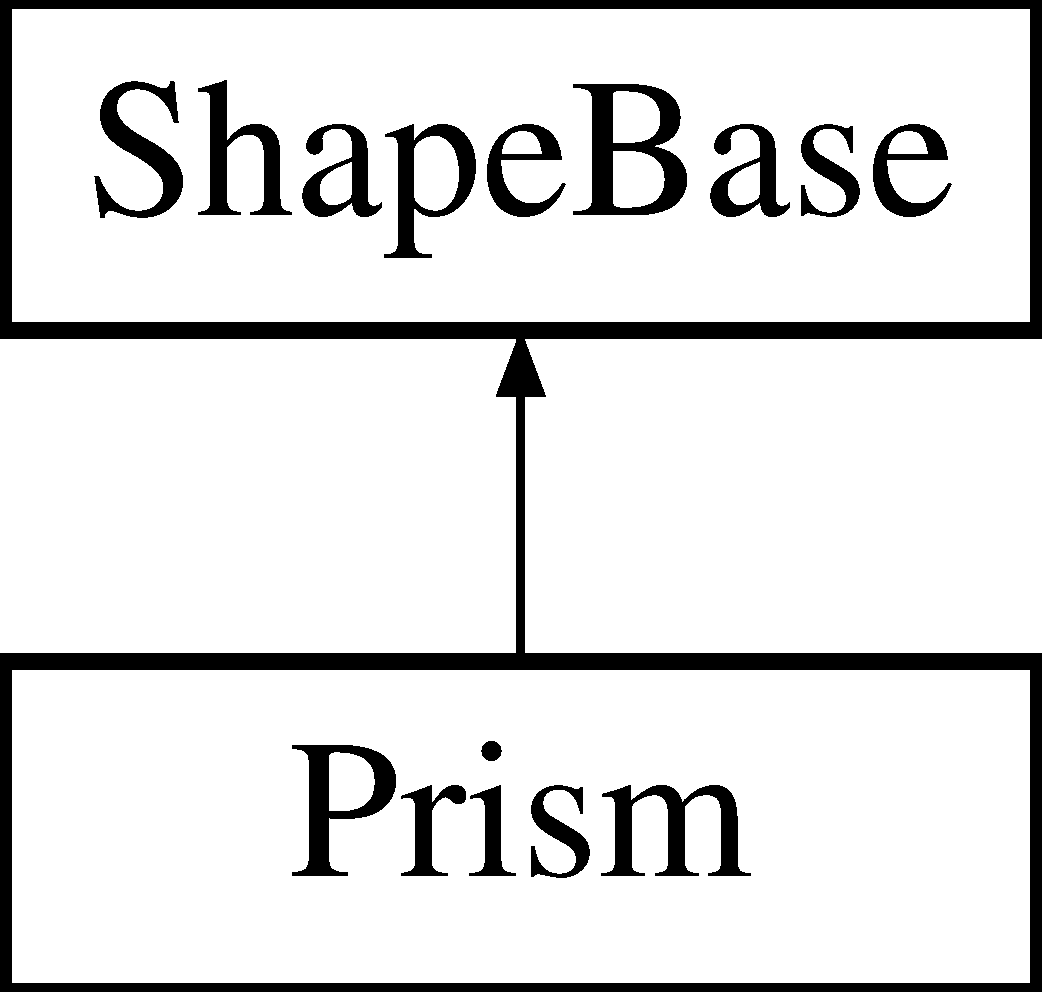
\includegraphics[height=2.000000cm]{classPrism}
\end{center}
\end{figure}
\subsection*{Public Member Functions}
\begin{DoxyCompactItemize}
\item 
\hypertarget{classPrism_aa107f8923cbbc9e1881cf98666743ae6}{}{\bfseries Prism} (int $\ast$Node\+Ids, vector$<$ \hyperlink{classNode}{Node} $\ast$ $>$ \&Nodes, int Curr\+Id)\label{classPrism_aa107f8923cbbc9e1881cf98666743ae6}

\item 
\hypertarget{classPrism_ab1eaaa559c1997fa7b30e84d7ce6b2d5}{}void {\bfseries set\+Elastic\+Properties} (double E\+Apical, double E\+Basal, double E\+Mid, double v)\label{classPrism_ab1eaaa559c1997fa7b30e84d7ce6b2d5}

\item 
\hypertarget{classPrism_aa65f89d72659c92de21c411a2fa23a7e}{}void {\bfseries calculate\+Basal\+Normal} (double $\ast$normal)\label{classPrism_aa65f89d72659c92de21c411a2fa23a7e}

\item 
\hypertarget{classPrism_a64100d877e59727ab9b7e9ad56e17cee}{}void {\bfseries Align\+Reference\+Base\+Normal\+To\+Z} ()\label{classPrism_a64100d877e59727ab9b7e9ad56e17cee}

\item 
\hypertarget{classPrism_a9a877cebf651015b88af641f1e045699}{}void {\bfseries calculate\+Element\+Shape\+Function\+Derivatives} ()\label{classPrism_a9a877cebf651015b88af641f1e045699}

\item 
\hypertarget{classPrism_af4ce210a9ba20d34b4b903e936b9dd8d}{}void {\bfseries check\+Health} ()\label{classPrism_af4ce210a9ba20d34b4b903e936b9dd8d}

\item 
\hypertarget{classPrism_ad9b04b2ad4cdedb878b4c7c0b4917a7a}{}void {\bfseries get\+Apical\+Triangles} (vector$<$ int $>$ \&Apical\+Triangles)\label{classPrism_ad9b04b2ad4cdedb878b4c7c0b4917a7a}

\item 
\hypertarget{classPrism_a10377e0ad0ae454a3cd25b82709119ac}{}int {\bfseries get\+Correcponding\+Apical} (int curr\+Node\+Id)\label{classPrism_a10377e0ad0ae454a3cd25b82709119ac}

\item 
\hypertarget{classPrism_abe648c5fa60635a50c14186135bed332}{}bool {\bfseries Is\+This\+Node\+My\+Basal} (int curr\+Node\+Id)\label{classPrism_abe648c5fa60635a50c14186135bed332}

\item 
\hypertarget{classPrism_a91d08cfcf6bf111f5d9e314499bafd11}{}double {\bfseries get\+Element\+Height} ()\label{classPrism_a91d08cfcf6bf111f5d9e314499bafd11}

\item 
\hypertarget{classPrism_aea2d84b05534bb2aedcdb49a53eab1ae}{}void {\bfseries Add\+Packing\+To\+Surface} (int tissueplacement\+Of\+Packing\+Node, double Fx, double Fy, double Fz, double $\ast$$\ast$Packing\+Forces, vector$<$ \hyperlink{classNode}{Node} $\ast$ $>$ \&Nodes, bool \&all\+Corners\+Fixed\+X, bool \&all\+Corners\+Fixed\+Y, bool \&all\+Corners\+Fixed\+Z)\label{classPrism_aea2d84b05534bb2aedcdb49a53eab1ae}

\item 
\hypertarget{classPrism_aa153c49304a9d808af5ea65a40f89128}{}void {\bfseries get\+Relevant\+Nodes\+For\+Packing} (int Tissue\+Placement\+Of\+Packing\+Node, int Tissue\+Type\+Of\+Packing\+Node, int \&id1, int \&id2, int \&id3)\label{classPrism_aa153c49304a9d808af5ea65a40f89128}

\item 
\hypertarget{classPrism_a45363ee4cc0dddd82ef567846a6bf123}{}bool {\bfseries Is\+Point\+Close\+Enough\+For\+Packing} (double $\ast$Pos, float threshold, int Tissue\+Placement\+Of\+Packing\+Node, int Tissue\+Type\+Of\+Packing\+Node)\label{classPrism_a45363ee4cc0dddd82ef567846a6bf123}

\item 
\hypertarget{classPrism_acb1603367b049392cebfc20b3aaeab87}{}void {\bfseries calculate\+Normal\+For\+Packing} (int tissue\+Placement\+Of\+Normal)\label{classPrism_acb1603367b049392cebfc20b3aaeab87}

\item 
\hypertarget{classPrism_a67e80515fb1cdf4438b4b7d47334bd2e}{}void {\bfseries calculate\+Apical\+Area} ()\label{classPrism_a67e80515fb1cdf4438b4b7d47334bd2e}

\item 
\hypertarget{classPrism_aa8dd4b90cdaecdbabfb48f45a9bcdc95}{}void {\bfseries calculate\+Basal\+Area} ()\label{classPrism_aa8dd4b90cdaecdbabfb48f45a9bcdc95}

\item 
\hypertarget{classPrism_a306261925defdb79ba64fc5f9ef8a23d}{}void {\bfseries calculate\+Myosin\+Forces} (double force\+Per\+Myo\+Molecule)\label{classPrism_a306261925defdb79ba64fc5f9ef8a23d}

\item 
\hypertarget{classPrism_ab11b5901fc7d65f71c7cccd1ce94a273}{}void {\bfseries distribute\+Myosin\+Force} (bool is\+Isotropic, bool apical, double force\+Per\+Myo\+Molecule)\label{classPrism_ab11b5901fc7d65f71c7cccd1ce94a273}

\item 
\hypertarget{classPrism_a243934a73a8f198ed592761ecb0927b9}{}void {\bfseries get\+Apical\+Node\+Pos} (double $\ast$pos\+Corner)\label{classPrism_a243934a73a8f198ed592761ecb0927b9}

\item 
\hypertarget{classPrism_a31324d23b37fa20911916ebb7ee1064d}{}void {\bfseries get\+Basal\+Node\+Pos} (double $\ast$pos\+Corner)\label{classPrism_a31324d23b37fa20911916ebb7ee1064d}

\item 
\hypertarget{classPrism_a26bb1eed04307a373ba87b48f1c1a3ca}{}bool {\bfseries Ispoint\+Inside\+Triangle} (int tissueplacement, double x, double y, double z)\label{classPrism_a26bb1eed04307a373ba87b48f1c1a3ca}

\item 
\hypertarget{classPrism_a85f9b472a3310e76ab0c76bd1fb7dd30}{}void {\bfseries check\+Rotation\+Consistency3\+D} ()\label{classPrism_a85f9b472a3310e76ab0c76bd1fb7dd30}

\end{DoxyCompactItemize}
\subsection*{Protected Member Functions}
\begin{DoxyCompactItemize}
\item 
\hypertarget{classPrism_a39d403ac6ffb6b56d5b2d07f8e9463a4}{}void {\bfseries set\+Tissue\+Coords\+Rotations\+Buffers} ()\label{classPrism_a39d403ac6ffb6b56d5b2d07f8e9463a4}

\item 
\hypertarget{classPrism_a3c252dc104a1ca7208b23c72737cd916}{}void {\bfseries get\+Curr\+Relaxed\+Shape} (gsl\+\_\+matrix $\ast$Curr\+Relaxed\+Shape)\label{classPrism_a3c252dc104a1ca7208b23c72737cd916}

\item 
\hypertarget{classPrism_aa1a4d3411d1f3dc05816ec01dcfa8310}{}void {\bfseries set\+Shape\+Function\+Derivatives} (gsl\+\_\+matrix $\ast$Shape\+Func\+Der, double eta, double zeta, double nu)\label{classPrism_aa1a4d3411d1f3dc05816ec01dcfa8310}

\item 
\hypertarget{classPrism_aa1f76f3cabdd00eb057f41cebbaa466d}{}void {\bfseries set\+Shape\+Function\+Derivative\+Stack} (gsl\+\_\+matrix $\ast$Shape\+Func\+Der, gsl\+\_\+matrix $\ast$Shape\+Func\+Der\+Stack)\label{classPrism_aa1f76f3cabdd00eb057f41cebbaa466d}

\item 
\hypertarget{classPrism_a0575442613f8b7d9428c58cef19ab219}{}void {\bfseries set\+Coeff\+Mat} ()\label{classPrism_a0575442613f8b7d9428c58cef19ab219}

\item 
\hypertarget{classPrism_aa433244f86cdf23a611a1adc3391c3f0}{}void {\bfseries calculate\+Currk} (boost\+::numeric\+::ublas\+::matrix$<$ double $>$ \&currk, boost\+::numeric\+::ublas\+::matrix$<$ double $>$ \&curr\+B, boost\+::numeric\+::ublas\+::matrix$<$ double $>$ \&curr\+B\+E, boost\+::numeric\+::ublas\+::matrix$<$ double $>$ \&curr\+Bo, double eta, double zeta, double nu)\label{classPrism_aa433244f86cdf23a611a1adc3391c3f0}

\item 
void \hyperlink{classPrism_a606fbf422f9d652e0f697ea93dc2e088}{calculate\+Curr\+Nodal\+Forces} (gsl\+\_\+matrix $\ast$gslcurrge, gsl\+\_\+matrix $\ast$gslcurrgv, gsl\+\_\+matrix $\ast$gslcurr\+F, gsl\+\_\+matrix $\ast$displacement\+Per\+Dt, int point\+No)
\item 
\hypertarget{classPrism_ae9403142a217a005a4d588a6e472be27}{}void {\bfseries calculate\+Curr\+Tri\+Point\+F\+For\+Rotation} (gsl\+\_\+matrix $\ast$curr\+F, int point\+No)\label{classPrism_ae9403142a217a005a4d588a6e472be27}

\item 
\hypertarget{classPrism_a872ce1e6304b1400d2d0e712af2a0131}{}void {\bfseries calculate\+Normal\+To\+Bottom} ()\label{classPrism_a872ce1e6304b1400d2d0e712af2a0131}

\item 
\hypertarget{classPrism_a2d8821dcd96009c95f06f34ee23ede7e}{}void {\bfseries calculate\+Reference\+Normal\+To\+Bottom} ()\label{classPrism_a2d8821dcd96009c95f06f34ee23ede7e}

\item 
\hypertarget{classPrism_ac3b85296d366eb4dd67406228c519caf}{}void {\bfseries calculate\+Normal\+To\+Top} ()\label{classPrism_ac3b85296d366eb4dd67406228c519caf}

\item 
\hypertarget{classPrism_a41a101de7bb2f75c5f9b44de23187593}{}void {\bfseries calculate\+Reference\+Normal\+To\+Top} ()\label{classPrism_a41a101de7bb2f75c5f9b44de23187593}

\item 
\hypertarget{classPrism_a6144314003601a688d81b0389ea1114e}{}void {\bfseries get\+Current\+Alignment\+Sides} (double $\ast$, double $\ast$)\label{classPrism_a6144314003601a688d81b0389ea1114e}

\item 
\hypertarget{classPrism_ab5fa417d944a6903b5bc9d2f53d4616a}{}void {\bfseries get\+Current\+Alignment\+Faces} (double $\ast$Ref\+Side, double $\ast$Shape\+Side, double $\ast$Ref\+Face, double $\ast$Shape\+Face)\label{classPrism_ab5fa417d944a6903b5bc9d2f53d4616a}

\item 
\hypertarget{classPrism_a4472375144e5e38a912af1fb4e2cc2d1}{}void {\bfseries update\+Alignment\+Turn} ()\label{classPrism_a4472375144e5e38a912af1fb4e2cc2d1}

\item 
\hypertarget{classPrism_a4ea58fd729a2bbef20530200978a8f75}{}void {\bfseries calculate\+Reference\+Volume} ()\label{classPrism_a4ea58fd729a2bbef20530200978a8f75}

\item 
\hypertarget{classPrism_a6b273d198e94039758a027b0dfb2c8af}{}void {\bfseries calculate\+Plane\+Normals} (double $\ast$$\ast$normals)\label{classPrism_a6b273d198e94039758a027b0dfb2c8af}

\item 
\hypertarget{classPrism_a13de4e8cefb58b3a33de4c2f7265a3b0}{}void {\bfseries assign\+Nodal\+Vector} (double $\ast$vec, int id0, int id1)\label{classPrism_a13de4e8cefb58b3a33de4c2f7265a3b0}

\item 
\hypertarget{classPrism_ac9695169749356654e847a022ce29aff}{}bool {\bfseries check\+Node\+Plane\+Consistency} (double $\ast$$\ast$normals)\label{classPrism_ac9695169749356654e847a022ce29aff}

\item 
\hypertarget{classPrism_acc59ccf5e1b5f459a8fb871c2a78fe8e}{}double {\bfseries get\+Apical\+Side\+Length\+Average} ()\label{classPrism_acc59ccf5e1b5f459a8fb871c2a78fe8e}

\end{DoxyCompactItemize}
\subsection*{Additional Inherited Members}


\subsection{Member Function Documentation}
\hypertarget{classPrism_a606fbf422f9d652e0f697ea93dc2e088}{}\index{Prism@{Prism}!calculate\+Curr\+Nodal\+Forces@{calculate\+Curr\+Nodal\+Forces}}
\index{calculate\+Curr\+Nodal\+Forces@{calculate\+Curr\+Nodal\+Forces}!Prism@{Prism}}
\subsubsection[{calculate\+Curr\+Nodal\+Forces}]{\setlength{\rightskip}{0pt plus 5cm}void Prism\+::calculate\+Curr\+Nodal\+Forces (
\begin{DoxyParamCaption}
\item[{gsl\+\_\+matrix $\ast$}]{gslcurrge, }
\item[{gsl\+\_\+matrix $\ast$}]{gslcurrgv, }
\item[{gsl\+\_\+matrix $\ast$}]{gslcurr\+F, }
\item[{gsl\+\_\+matrix $\ast$}]{displacement\+Per\+Dt, }
\item[{int}]{point\+No}
\end{DoxyParamCaption}
)\hspace{0.3cm}{\ttfamily [protected]}, {\ttfamily [virtual]}}\label{classPrism_a606fbf422f9d652e0f697ea93dc2e088}
$<$ Removing growth

$<$ Removing shape change

$<$ Removing shape change 

Reimplemented from \hyperlink{classShapeBase}{Shape\+Base}.



The documentation for this class was generated from the following files\+:\begin{DoxyCompactItemize}
\item 
/home/melda/\+Documents/\+Tissue\+Folding/\+Tissue\+Folding/\+Source\+Code/Prism.\+h\item 
/home/melda/\+Documents/\+Tissue\+Folding/\+Tissue\+Folding/\+Source\+Code/Prism.\+cpp\end{DoxyCompactItemize}

\hypertarget{classReferenceShapeBase}{}\section{Reference\+Shape\+Base Class Reference}
\label{classReferenceShapeBase}\index{Reference\+Shape\+Base@{Reference\+Shape\+Base}}
\subsection*{Public Member Functions}
\begin{DoxyCompactItemize}
\item 
\hypertarget{classReferenceShapeBase_a3d27b5bf4c591a5973b466d2af08a118}{}\hyperlink{classReferenceShapeBase_a3d27b5bf4c591a5973b466d2af08a118}{Reference\+Shape\+Base} (string Syape\+Type, int \hyperlink{classReferenceShapeBase_af0da93cee3f17800d7aa90b21b1b81c7}{Id})\label{classReferenceShapeBase_a3d27b5bf4c591a5973b466d2af08a118}

\begin{DoxyCompactList}\small\item\em Constructer of the \hyperlink{classReferenceShapeBase}{Reference\+Shape\+Base} class. \end{DoxyCompactList}\item 
\hypertarget{classReferenceShapeBase_addf60ebee57a9d3b0e345b963901e3b5}{}\hyperlink{classReferenceShapeBase_addf60ebee57a9d3b0e345b963901e3b5}{$\sim$\+Reference\+Shape\+Base} ()\label{classReferenceShapeBase_addf60ebee57a9d3b0e345b963901e3b5}

\begin{DoxyCompactList}\small\item\em Destructor of the \hyperlink{classReferenceShapeBase}{Reference\+Shape\+Base} class. \end{DoxyCompactList}\end{DoxyCompactItemize}
\subsection*{Public Attributes}
\begin{DoxyCompactItemize}
\item 
\hypertarget{classReferenceShapeBase_a745e71ff73ef758708f39a4b3b1be4d1}{}double $\ast$$\ast$ \hyperlink{classReferenceShapeBase_a745e71ff73ef758708f39a4b3b1be4d1}{Positions}\label{classReferenceShapeBase_a745e71ff73ef758708f39a4b3b1be4d1}

\begin{DoxyCompactList}\small\item\em The pointer to the position matrix of the reference element. The array itself is declared within the constructor, depending on \hyperlink{classShapeBase_a250bd3396546342c8104f5b9c180d18f}{Shape\+Base\+::n\+Dim} and \hyperlink{classShapeBase_ae7dd93b58b3281ce90025f83d0f0e976}{Shape\+Base\+::n\+Nodes}, its size being \mbox{[}n\+Nodes\mbox{]}\mbox{[}n\+Dim\mbox{]}. \end{DoxyCompactList}\item 
\hypertarget{classReferenceShapeBase_a12d2d0c2511f4f1357360ff61910ac02}{}double \hyperlink{classReferenceShapeBase_a12d2d0c2511f4f1357360ff61910ac02}{Volume}\label{classReferenceShapeBase_a12d2d0c2511f4f1357360ff61910ac02}

\begin{DoxyCompactList}\small\item\em The volume of reference element, calculated assuming regular shapes (e.\+g. Perpendicular prism of equal top and bottom surfaces). \end{DoxyCompactList}\item 
\hypertarget{classReferenceShapeBase_a214b89b970efa7a290dbe1533cf237ea}{}double \hyperlink{classReferenceShapeBase_a214b89b970efa7a290dbe1533cf237ea}{Basal\+Area}\label{classReferenceShapeBase_a214b89b970efa7a290dbe1533cf237ea}

\begin{DoxyCompactList}\small\item\em The basal area of the reference shape. \end{DoxyCompactList}\item 
\hypertarget{classReferenceShapeBase_a76ac694d1b1276f6847bee3c3efa84b0}{}double \hyperlink{classReferenceShapeBase_a76ac694d1b1276f6847bee3c3efa84b0}{height}\label{classReferenceShapeBase_a76ac694d1b1276f6847bee3c3efa84b0}

\begin{DoxyCompactList}\small\item\em Slab height for 2\+D elements, value is -\/100 for 3\+D elements. Is obsolete now, must be deleted together with any 2\+D element option. Mesh file reading should be cleared in parallel. \end{DoxyCompactList}\end{DoxyCompactItemize}
\subsection*{Protected Member Functions}
\begin{DoxyCompactItemize}
\item 
\hypertarget{classReferenceShapeBase_ad893cb0986899d77de34ce5e565ebb97}{}void {\bfseries set\+Shape\+Type} (string Type\+Name)\label{classReferenceShapeBase_ad893cb0986899d77de34ce5e565ebb97}

\item 
\hypertarget{classReferenceShapeBase_a027db08b5e580286448380aa21902b33}{}void {\bfseries set\+Node\+Number} ()\label{classReferenceShapeBase_a027db08b5e580286448380aa21902b33}

\end{DoxyCompactItemize}
\subsection*{Protected Attributes}
\begin{DoxyCompactItemize}
\item 
\hypertarget{classReferenceShapeBase_a4831a54cffbafef4ded26fb8c50566e0}{}int \hyperlink{classReferenceShapeBase_a4831a54cffbafef4ded26fb8c50566e0}{Shape\+Type}\label{classReferenceShapeBase_a4831a54cffbafef4ded26fb8c50566e0}

\begin{DoxyCompactList}\small\item\em The integer defining the type of the shape, it is a negative value at the same basis of \hyperlink{classShapeBase_a36aedd41e8465a186a0b0c454b5b76f3}{Shape\+Base\+::\+Shape\+Type}\+: prisms Shape\+Type = -\/1. \end{DoxyCompactList}\item 
\hypertarget{classReferenceShapeBase_af0da93cee3f17800d7aa90b21b1b81c7}{}int \hyperlink{classReferenceShapeBase_af0da93cee3f17800d7aa90b21b1b81c7}{Id}\label{classReferenceShapeBase_af0da93cee3f17800d7aa90b21b1b81c7}

\begin{DoxyCompactList}\small\item\em The unique identifier of the reference shape, it is identical to the owner shape, it is set inside the constructor. \end{DoxyCompactList}\item 
\hypertarget{classReferenceShapeBase_a1183c092056a3245a350ff6f56632633}{}int \hyperlink{classReferenceShapeBase_a1183c092056a3245a350ff6f56632633}{n\+Nodes}\label{classReferenceShapeBase_a1183c092056a3245a350ff6f56632633}

\begin{DoxyCompactList}\small\item\em The number of nodes of the reference element, it is based on \hyperlink{classReferenceShapeBase_a4831a54cffbafef4ded26fb8c50566e0}{Reference\+Shape\+Base\+::\+Shape\+Type}, through function Reference\+Shape\+Base\+::set\+Node\+Number. \end{DoxyCompactList}\end{DoxyCompactItemize}


The documentation for this class was generated from the following files\+:\begin{DoxyCompactItemize}
\item 
/home/melda/\+Documents/\+Tissue\+Folding/\+Tissue\+Folding/\+Source\+Code/Reference\+Shape\+Base.\+h\item 
/home/melda/\+Documents/\+Tissue\+Folding/\+Tissue\+Folding/\+Source\+Code/Reference\+Shape\+Base.\+cpp\end{DoxyCompactItemize}

\hypertarget{classRingGrowthFunction}{}\section{Ring\+Growth\+Function Class Reference}
\label{classRingGrowthFunction}\index{Ring\+Growth\+Function@{Ring\+Growth\+Function}}
Inheritance diagram for Ring\+Growth\+Function\+:\begin{figure}[H]
\begin{center}
\leavevmode
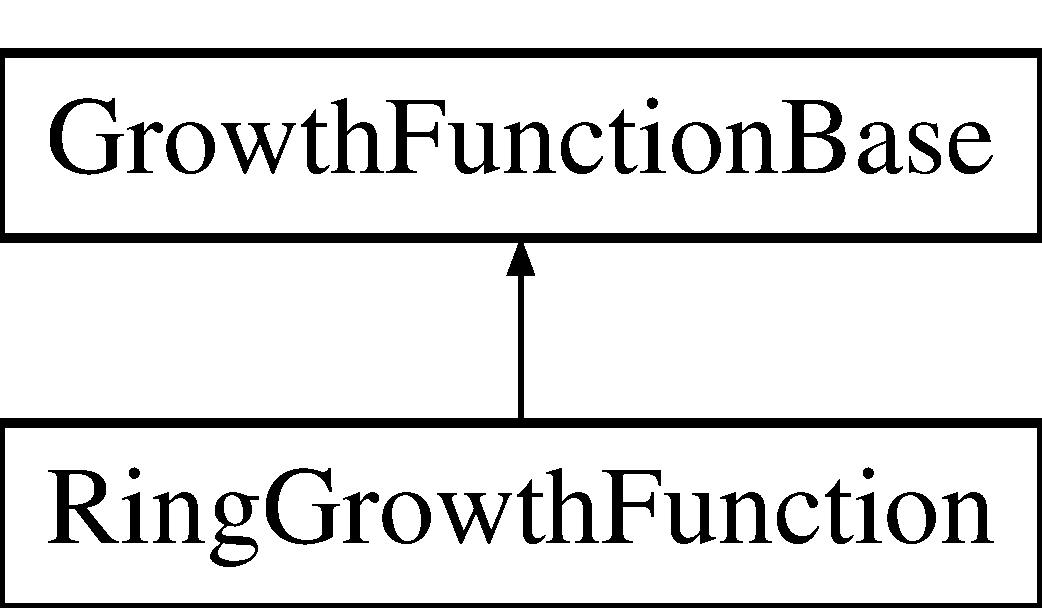
\includegraphics[height=2.000000cm]{classRingGrowthFunction}
\end{center}
\end{figure}
\subsection*{Public Member Functions}
\begin{DoxyCompactItemize}
\item 
\hyperlink{classRingGrowthFunction_a6d4914efe62137aae9fec55401edf986}{Ring\+Growth\+Function} (int id, int type, float \hyperlink{classGrowthFunctionBase_ae92513a7b41637df8e26e7db35ddf97c}{init\+Time}, float \hyperlink{classGrowthFunctionBase_a3ff4db0573d354a75666a5f3ca446941}{end\+Time}, bool \hyperlink{classGrowthFunctionBase_a3d56771e7c145589a14e11cc331e0326}{apply\+To\+Columnar\+Layer}, bool \hyperlink{classGrowthFunctionBase_a08ae19f58cb98fa8e315a77f52749732}{apply\+To\+Peripodial\+Membrane}, bool \hyperlink{classGrowthFunctionBase_a9fe46fc6dde4041b79204beb48972a09}{apply\+To\+Basal\+E\+C\+M}, bool \hyperlink{classGrowthFunctionBase_ac623b1dbe376bce5dddbe1a2e21c776f}{apply\+To\+Lateral\+E\+C\+M}, double Cx, double Cy, double inner\+R, double outer\+R, double D\+V\+Growth, double A\+P\+Growth, double A\+B\+Growth, double \hyperlink{classRingGrowthFunction_add6283d1ad999925c4202a3fa66b76ea}{angle})
\begin{DoxyCompactList}\small\item\em The constructor of \hyperlink{classRingGrowthFunction}{Ring\+Growth\+Function}. \end{DoxyCompactList}\item 
\hypertarget{classRingGrowthFunction_aa2063170e3ee5c5f22d7beef32300e9c}{}void \hyperlink{classRingGrowthFunction_aa2063170e3ee5c5f22d7beef32300e9c}{get\+Centre} (float \&centre\+X, float \&centre\+Y)\label{classRingGrowthFunction_aa2063170e3ee5c5f22d7beef32300e9c}

\begin{DoxyCompactList}\small\item\em This function writes \hyperlink{classRingGrowthFunction_a5b8f1cc72d03907bb1492e6c2f288db0}{Ring\+Growth\+Function\+::centre} into the input float addresses centre\+X and centre\+Y, in this order. \end{DoxyCompactList}\item 
\hypertarget{classRingGrowthFunction_ae1f4f4cecfab3ec343c748cfe78ab70b}{}float \hyperlink{classRingGrowthFunction_ae1f4f4cecfab3ec343c748cfe78ab70b}{get\+Inner\+Radius} ()\label{classRingGrowthFunction_ae1f4f4cecfab3ec343c748cfe78ab70b}

\begin{DoxyCompactList}\small\item\em This function returns \hyperlink{classRingGrowthFunction_a4e8796fbbbe9fe18c2dcd04613effcf0}{Ring\+Growth\+Function\+::inner\+Radius}. \end{DoxyCompactList}\item 
\hypertarget{classRingGrowthFunction_ad5c890c72a8ce520411d28e929faec19}{}float \hyperlink{classRingGrowthFunction_ad5c890c72a8ce520411d28e929faec19}{get\+Outer\+Radius} ()\label{classRingGrowthFunction_ad5c890c72a8ce520411d28e929faec19}

\begin{DoxyCompactList}\small\item\em This function returns \hyperlink{classRingGrowthFunction_a8b7d5268d9d47f112b56feef58193649}{Ring\+Growth\+Function\+::outer\+Radius}. \end{DoxyCompactList}\item 
void \hyperlink{classRingGrowthFunction_ab3cc1858fb602ab40a74af7d0467c13b}{get\+Growth\+Rate} (double $\ast$max\+Values)
\begin{DoxyCompactList}\small\item\em The function is to set the 3\+D maximum growth rate of the current ring growth function. \end{DoxyCompactList}\item 
void \hyperlink{classRingGrowthFunction_a051da280e649c81afff38a1a45cb035a}{set\+Growt\+Rate} (double ex, double ey, double ez)
\begin{DoxyCompactList}\small\item\em The function is to set the 3\+D maximum growth rate of the current ring growth function. \end{DoxyCompactList}\item 
\hypertarget{classRingGrowthFunction_a05f880ba6df8b3001a8e8fdec5ba1ad6}{}gsl\+\_\+matrix $\ast$ \hyperlink{classRingGrowthFunction_a05f880ba6df8b3001a8e8fdec5ba1ad6}{get\+Shear\+Angle\+Rotation\+Matrix} ()\label{classRingGrowthFunction_a05f880ba6df8b3001a8e8fdec5ba1ad6}

\begin{DoxyCompactList}\small\item\em The function return the matrix pointer to the oriented growth rotation matrix. \end{DoxyCompactList}\item 
\hypertarget{classRingGrowthFunction_aa70523c66dce48e7e54360596787a629}{}double \hyperlink{classRingGrowthFunction_aa70523c66dce48e7e54360596787a629}{get\+Shear\+Angle} ()\label{classRingGrowthFunction_aa70523c66dce48e7e54360596787a629}

\begin{DoxyCompactList}\small\item\em The function returns the oriented growth angle in radians (double). \end{DoxyCompactList}\item 
void \hyperlink{classRingGrowthFunction_a681175045cf09fadd92921e129737e65}{write\+Summary} (ofstream \&save\+File\+Simulation\+Summary, double dt)
\begin{DoxyCompactList}\small\item\em The function is to write the growth function summary to simulation summary file. \end{DoxyCompactList}\end{DoxyCompactItemize}
\subsection*{Public Attributes}
\begin{DoxyCompactItemize}
\item 
\hypertarget{classRingGrowthFunction_a5b8f1cc72d03907bb1492e6c2f288db0}{}double \hyperlink{classRingGrowthFunction_a5b8f1cc72d03907bb1492e6c2f288db0}{centre} \mbox{[}2\mbox{]}\label{classRingGrowthFunction_a5b8f1cc72d03907bb1492e6c2f288db0}

\begin{DoxyCompactList}\small\item\em The double array of 2, giving the centre of the ring in micro-\/meters, format \mbox{[}x, y\mbox{]}. \end{DoxyCompactList}\item 
\hypertarget{classRingGrowthFunction_a4e8796fbbbe9fe18c2dcd04613effcf0}{}double \hyperlink{classRingGrowthFunction_a4e8796fbbbe9fe18c2dcd04613effcf0}{inner\+Radius}\label{classRingGrowthFunction_a4e8796fbbbe9fe18c2dcd04613effcf0}

\begin{DoxyCompactList}\small\item\em The inner radius of the ring, inner boundary of the growth region in micro-\/meters. The growth will be zero at and inside the inner radius. This value can be set to zero to have circular growth. \end{DoxyCompactList}\item 
\hypertarget{classRingGrowthFunction_a8b7d5268d9d47f112b56feef58193649}{}double \hyperlink{classRingGrowthFunction_a8b7d5268d9d47f112b56feef58193649}{outer\+Radius}\label{classRingGrowthFunction_a8b7d5268d9d47f112b56feef58193649}

\begin{DoxyCompactList}\small\item\em The outer radius of the ring, outer boundary of the growth region in micro-\/meters. The growth will be at the maximum value set by \hyperlink{classRingGrowthFunction_a93b70ff6a7258c73a6bd2d888d09fc09}{Ring\+Growth\+Function\+::\+Growth\+Rate} at the outer radius. \end{DoxyCompactList}\item 
\hypertarget{classRingGrowthFunction_a93b70ff6a7258c73a6bd2d888d09fc09}{}double \hyperlink{classRingGrowthFunction_a93b70ff6a7258c73a6bd2d888d09fc09}{Growth\+Rate} \mbox{[}3\mbox{]}\label{classRingGrowthFunction_a93b70ff6a7258c73a6bd2d888d09fc09}

\begin{DoxyCompactList}\small\item\em The maximum growth rate at the \hyperlink{classRingGrowthFunction_a8b7d5268d9d47f112b56feef58193649}{Ring\+Growth\+Function\+::outer\+Radius}, in (1/sec), format\+: \mbox{[} D\+V axis (x), A\+P axis (y), and A\+B axis (z)\mbox{]}. \end{DoxyCompactList}\item 
\hypertarget{classRingGrowthFunction_a9603e5de21f7bca0c23deff2c1e9efd6}{}gsl\+\_\+matrix $\ast$ \hyperlink{classRingGrowthFunction_a9603e5de21f7bca0c23deff2c1e9efd6}{Shear\+Angle\+Rotation\+Matrix}\label{classRingGrowthFunction_a9603e5de21f7bca0c23deff2c1e9efd6}

\begin{DoxyCompactList}\small\item\em The rotation matrix for the orientation of the growth on x-\/y plane. This matrix is constructed through \hyperlink{classUniformGrowthFunction_a1a985ff52f9796688e00942b4d3349f8}{Uniform\+Growth\+Function\+::angle}. \end{DoxyCompactList}\item 
\hypertarget{classRingGrowthFunction_add6283d1ad999925c4202a3fa66b76ea}{}double \hyperlink{classRingGrowthFunction_add6283d1ad999925c4202a3fa66b76ea}{angle}\label{classRingGrowthFunction_add6283d1ad999925c4202a3fa66b76ea}

\begin{DoxyCompactList}\small\item\em The rotation angle for the orientation of the growth on x-\/y plane. \end{DoxyCompactList}\end{DoxyCompactItemize}


\subsection{Constructor \& Destructor Documentation}
\hypertarget{classRingGrowthFunction_a6d4914efe62137aae9fec55401edf986}{}\index{Ring\+Growth\+Function@{Ring\+Growth\+Function}!Ring\+Growth\+Function@{Ring\+Growth\+Function}}
\index{Ring\+Growth\+Function@{Ring\+Growth\+Function}!Ring\+Growth\+Function@{Ring\+Growth\+Function}}
\subsubsection[{Ring\+Growth\+Function}]{\setlength{\rightskip}{0pt plus 5cm}Ring\+Growth\+Function\+::\+Ring\+Growth\+Function (
\begin{DoxyParamCaption}
\item[{int}]{id, }
\item[{int}]{type, }
\item[{float}]{init\+Time, }
\item[{float}]{end\+Time, }
\item[{bool}]{apply\+To\+Columnar\+Layer, }
\item[{bool}]{apply\+To\+Peripodial\+Membrane, }
\item[{bool}]{apply\+To\+Basal\+E\+C\+M, }
\item[{bool}]{apply\+To\+Lateral\+E\+C\+M, }
\item[{double}]{Cx, }
\item[{double}]{Cy, }
\item[{double}]{inner\+R, }
\item[{double}]{outer\+R, }
\item[{double}]{D\+V\+Growth, }
\item[{double}]{A\+P\+Growth, }
\item[{double}]{A\+B\+Growth, }
\item[{double}]{angle}
\end{DoxyParamCaption}
)\hspace{0.3cm}{\ttfamily [inline]}}\label{classRingGrowthFunction_a6d4914efe62137aae9fec55401edf986}


The constructor of \hyperlink{classRingGrowthFunction}{Ring\+Growth\+Function}. 

The first six parameters will be directed to the parent constructor, \hyperlink{classGrowthFunctionBase_a5c275b3f839cc4f572b68afc5ad1064f}{Growth\+Function\+Base\+::\+Growth\+Function\+Base}. ~\newline
doubles Cx and Cy will set \hyperlink{classRingGrowthFunction_a5b8f1cc72d03907bb1492e6c2f288db0}{Ring\+Growth\+Function\+::centre}\mbox{[}0\mbox{]} and \hyperlink{classRingGrowthFunction_a5b8f1cc72d03907bb1492e6c2f288db0}{Ring\+Growth\+Function\+::centre}\mbox{[}1\mbox{]}, respectively. ~\newline
doubles inner\+R and outer\+R will set \hyperlink{classRingGrowthFunction_a4e8796fbbbe9fe18c2dcd04613effcf0}{Ring\+Growth\+Function\+::inner\+Radius} and \hyperlink{classRingGrowthFunction_a8b7d5268d9d47f112b56feef58193649}{Ring\+Growth\+Function\+::outer\+Radius}, respectively. ~\newline
doubles D\+V\+Growth, A\+P\+Growth and A\+B\+Growth will set the \hyperlink{classRingGrowthFunction_a93b70ff6a7258c73a6bd2d888d09fc09}{Ring\+Growth\+Function\+::\+Growth\+Rate}, in the given order.

\subsection{Member Function Documentation}
\hypertarget{classRingGrowthFunction_ab3cc1858fb602ab40a74af7d0467c13b}{}\index{Ring\+Growth\+Function@{Ring\+Growth\+Function}!get\+Growth\+Rate@{get\+Growth\+Rate}}
\index{get\+Growth\+Rate@{get\+Growth\+Rate}!Ring\+Growth\+Function@{Ring\+Growth\+Function}}
\subsubsection[{get\+Growth\+Rate}]{\setlength{\rightskip}{0pt plus 5cm}void Ring\+Growth\+Function\+::get\+Growth\+Rate (
\begin{DoxyParamCaption}
\item[{double $\ast$}]{max\+Values}
\end{DoxyParamCaption}
)\hspace{0.3cm}{\ttfamily [inline]}, {\ttfamily [virtual]}}\label{classRingGrowthFunction_ab3cc1858fb602ab40a74af7d0467c13b}


The function is to set the 3\+D maximum growth rate of the current ring growth function. 

This function will write the \hyperlink{classRingGrowthFunction_a93b70ff6a7258c73a6bd2d888d09fc09}{Ring\+Growth\+Function\+::\+Growth\+Rate} of the current growth function to the input double array pointer. The double array pointer should be set to point at a double array of size 3 (or higher) before calling the function.

Reimplemented from \hyperlink{classGrowthFunctionBase_a2c518c297bc1bbf996f6e7df758a0cc7}{Growth\+Function\+Base}.

\hypertarget{classRingGrowthFunction_a051da280e649c81afff38a1a45cb035a}{}\index{Ring\+Growth\+Function@{Ring\+Growth\+Function}!set\+Growt\+Rate@{set\+Growt\+Rate}}
\index{set\+Growt\+Rate@{set\+Growt\+Rate}!Ring\+Growth\+Function@{Ring\+Growth\+Function}}
\subsubsection[{set\+Growt\+Rate}]{\setlength{\rightskip}{0pt plus 5cm}void Ring\+Growth\+Function\+::set\+Growt\+Rate (
\begin{DoxyParamCaption}
\item[{double}]{ex, }
\item[{double}]{ey, }
\item[{double}]{ez}
\end{DoxyParamCaption}
)\hspace{0.3cm}{\ttfamily [inline]}, {\ttfamily [virtual]}}\label{classRingGrowthFunction_a051da280e649c81afff38a1a45cb035a}


The function is to set the 3\+D maximum growth rate of the current ring growth function. 

This function will set the \hyperlink{classRingGrowthFunction_a93b70ff6a7258c73a6bd2d888d09fc09}{Ring\+Growth\+Function\+::\+Growth\+Rate} of the current growth function to the input values The parameters are in the order \mbox{[} D\+V axis (x), A\+P axis (y), and A\+B axis (z)\mbox{]}.

Reimplemented from \hyperlink{classGrowthFunctionBase}{Growth\+Function\+Base}.

\hypertarget{classRingGrowthFunction_a681175045cf09fadd92921e129737e65}{}\index{Ring\+Growth\+Function@{Ring\+Growth\+Function}!write\+Summary@{write\+Summary}}
\index{write\+Summary@{write\+Summary}!Ring\+Growth\+Function@{Ring\+Growth\+Function}}
\subsubsection[{write\+Summary}]{\setlength{\rightskip}{0pt plus 5cm}void Ring\+Growth\+Function\+::write\+Summary (
\begin{DoxyParamCaption}
\item[{ofstream \&}]{save\+File\+Simulation\+Summary, }
\item[{double}]{dt}
\end{DoxyParamCaption}
)\hspace{0.3cm}{\ttfamily [inline]}, {\ttfamily [virtual]}}\label{classRingGrowthFunction_a681175045cf09fadd92921e129737e65}


The function is to write the growth function summary to simulation summary file. 

This function will write the \hyperlink{classRingGrowthFunction}{Ring\+Growth\+Function} details into the simulation summary file, provided as the first input. Time step (dt) of the simulation is provided as second input, to report the growth rates per hour. The output should look like\+: ~\newline
 Growth Type\+: Ring (2) Initial time(sec)\+: \hyperlink{classGrowthFunctionBase_ae92513a7b41637df8e26e7db35ddf97c}{Ring\+Growth\+Function\+::init\+Time} Final\+Time time(sec)\+: \hyperlink{classGrowthFunctionBase_a3ff4db0573d354a75666a5f3ca446941}{Ring\+Growth\+Function\+::end\+Time} Centre(micron)\+: \hyperlink{classRingGrowthFunction_a5b8f1cc72d03907bb1492e6c2f288db0}{Ring\+Growth\+Function\+::centre}\mbox{[}0\mbox{]} \hyperlink{classRingGrowthFunction_a5b8f1cc72d03907bb1492e6c2f288db0}{Ring\+Growth\+Function\+::centre}\mbox{[}1\mbox{]} Inner radius(micron)\+: \hyperlink{classRingGrowthFunction_a4e8796fbbbe9fe18c2dcd04613effcf0}{Ring\+Growth\+Function\+::inner\+Radius} Outer radius(micron)\+: \hyperlink{classRingGrowthFunction_a8b7d5268d9d47f112b56feef58193649}{Ring\+Growth\+Function\+::outer\+Radius} Growth\+Rate(fraction/hr)\+:D\+V\+Growth(in 1/hr) A\+P\+Growth(in 1/hr) A\+B\+Growth(in 1/hr)

Reimplemented from \hyperlink{classGrowthFunctionBase_a73b474a60caeb5b6b326ecb6a056cfe4}{Growth\+Function\+Base}.



The documentation for this class was generated from the following file\+:\begin{DoxyCompactItemize}
\item 
/home/melda/\+Documents/\+Tissue\+Folding/\+Tissue\+Folding/\+Source\+Code/Growth\+Function\+Types.\+h\end{DoxyCompactItemize}

\hypertarget{classShapeBase}{}\section{Shape\+Base Class Reference}
\label{classShapeBase}\index{Shape\+Base@{Shape\+Base}}
Inheritance diagram for Shape\+Base\+:\begin{figure}[H]
\begin{center}
\leavevmode
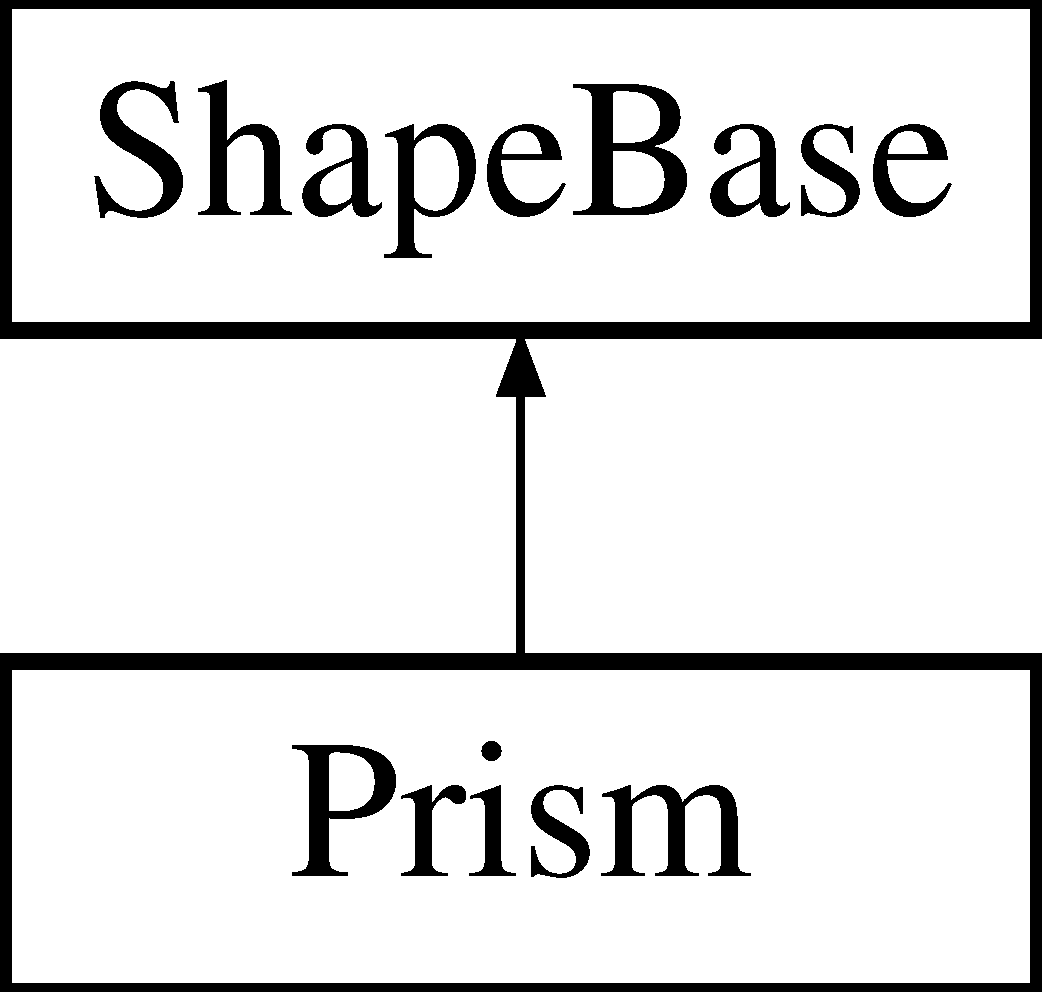
\includegraphics[height=2.000000cm]{classShapeBase}
\end{center}
\end{figure}
\subsection*{Public Member Functions}
\begin{DoxyCompactItemize}
\item 
\hypertarget{classShapeBase_ab55ac0089ea8e37649b0d85409c008ac}{}int {\bfseries get\+Id} ()\label{classShapeBase_ab55ac0089ea8e37649b0d85409c008ac}

\item 
\hypertarget{classShapeBase_a49d134532a98fb0cecacec44baf2baf3}{}string {\bfseries get\+Name} ()\label{classShapeBase_a49d134532a98fb0cecacec44baf2baf3}

\item 
\hypertarget{classShapeBase_a7ae6deee4256eb19c6e99b52a40847cb}{}int {\bfseries get\+Shape\+Type} ()\label{classShapeBase_a7ae6deee4256eb19c6e99b52a40847cb}

\item 
\hypertarget{classShapeBase_a46ce732af56537977ce6a34832440309}{}int {\bfseries get\+Node\+Number} ()\label{classShapeBase_a46ce732af56537977ce6a34832440309}

\item 
\hypertarget{classShapeBase_a55c283eaee304f9056089987e9b65012}{}int $\ast$ {\bfseries get\+Node\+Ids} ()\label{classShapeBase_a55c283eaee304f9056089987e9b65012}

\item 
\hypertarget{classShapeBase_ad60d92b34044153a677a8bfc0a31a5df}{}int {\bfseries get\+Dim} ()\label{classShapeBase_ad60d92b34044153a677a8bfc0a31a5df}

\item 
\hypertarget{classShapeBase_af10ec5e87cab16541c892712cf58c54d}{}int $\ast$ {\bfseries get\+Identifier\+Colour} ()\label{classShapeBase_af10ec5e87cab16541c892712cf58c54d}

\item 
\hypertarget{classShapeBase_ab26e6cbde2c8a4f326c32a38de48bcc7}{}double $\ast$ {\bfseries get\+Centre} ()\label{classShapeBase_ab26e6cbde2c8a4f326c32a38de48bcc7}

\item 
\hypertarget{classShapeBase_a7d1235b3555a18328d1677e5b07458ff}{}void {\bfseries calculate\+Relative\+Pos\+In\+Bounding\+Box} (double Boinding\+Box\+X\+Min, double Bounding\+Box\+Y\+Min, double Bounding\+Box\+Length, double Bounding\+Box\+Width)\label{classShapeBase_a7d1235b3555a18328d1677e5b07458ff}

\item 
\hypertarget{classShapeBase_ae5e17514271f121498ed12cebae3aebe}{}void {\bfseries display\+Relative\+Pos\+In\+Bounding\+Box} ()\label{classShapeBase_ae5e17514271f121498ed12cebae3aebe}

\item 
\hypertarget{classShapeBase_a0d33afa938cd84b1376806a06769f6b9}{}void {\bfseries get\+Relative\+Pos\+In\+Bounding\+Box} (double $\ast$relative\+Pos)\label{classShapeBase_a0d33afa938cd84b1376806a06769f6b9}

\item 
\hypertarget{classShapeBase_aecf99016ea7c36e0bff43a40e6a89df3}{}void {\bfseries get\+Strain} (int type, float \&Strain\+Mag)\label{classShapeBase_aecf99016ea7c36e0bff43a40e6a89df3}

\item 
\hypertarget{classShapeBase_ac1368b84a5ed722fa7b9f82656b49969}{}void {\bfseries get\+Node\+Based\+Pys\+Prop} (int type, int Node\+No, vector$<$ \hyperlink{classNode}{Node} $\ast$ $>$ \&Nodes, float \&Pys\+Prop\+Mag)\label{classShapeBase_ac1368b84a5ed722fa7b9f82656b49969}

\item 
\hypertarget{classShapeBase_abff91451c3465778ed89624d6196f7f6}{}void {\bfseries get\+Pys\+Prop} (int type, float \&Pys\+Prop\+Mag, double dt)\label{classShapeBase_abff91451c3465778ed89624d6196f7f6}

\item 
\hypertarget{classShapeBase_ade96ff86461eaabce716e83fa68bfa19}{}double {\bfseries get\+Young\+Modulus} ()\label{classShapeBase_ade96ff86461eaabce716e83fa68bfa19}

\item 
\hypertarget{classShapeBase_a01140f17779cd2e990c9f28e3c86b77e}{}double {\bfseries get\+Poisson\+Ratio} ()\label{classShapeBase_a01140f17779cd2e990c9f28e3c86b77e}

\item 
\hypertarget{classShapeBase_a94b472ab0c5242226313cd096e17a3fe}{}double $\ast$ {\bfseries get\+Growth\+Rate} ()\label{classShapeBase_a94b472ab0c5242226313cd096e17a3fe}

\item 
\hypertarget{classShapeBase_a6f4d5556ac05b897919f49dacd0f8101}{}double $\ast$ {\bfseries get\+Shape\+Change\+Rate} ()\label{classShapeBase_a6f4d5556ac05b897919f49dacd0f8101}

\item 
\hypertarget{classShapeBase_a91ba74cc41917dbe821159023f1bf1ec}{}double $\ast$$\ast$ {\bfseries get\+Reference\+Pos} ()\label{classShapeBase_a91ba74cc41917dbe821159023f1bf1ec}

\item 
\hypertarget{classShapeBase_ab1906a5afda8fcbeef23010759f2538c}{}void {\bfseries get\+Pos} (gsl\+\_\+matrix $\ast$Pos)\label{classShapeBase_ab1906a5afda8fcbeef23010759f2538c}

\item 
\hypertarget{classShapeBase_a79889ef9cb7831a50e5391cb1cc19793}{}gsl\+\_\+matrix $\ast$ {\bfseries get\+Fg} ()\label{classShapeBase_a79889ef9cb7831a50e5391cb1cc19793}

\item 
\hypertarget{classShapeBase_ab8a7323c50767ecdc82d8d8ce411b264}{}void {\bfseries display\+Name} ()\label{classShapeBase_ab8a7323c50767ecdc82d8d8ce411b264}

\item 
\hypertarget{classShapeBase_a324f8fd5dd90c14b621b2f2ee3ec98db}{}void {\bfseries display\+Node\+Ids} ()\label{classShapeBase_a324f8fd5dd90c14b621b2f2ee3ec98db}

\item 
\hypertarget{classShapeBase_aca4d0f70caf459dc93f914ef7fc2a053}{}void {\bfseries display\+Positions} ()\label{classShapeBase_aca4d0f70caf459dc93f914ef7fc2a053}

\item 
\hypertarget{classShapeBase_af2d221cf63220dad3ecf139ffa164698}{}void {\bfseries display\+Reference\+Positions} ()\label{classShapeBase_af2d221cf63220dad3ecf139ffa164698}

\item 
\hypertarget{classShapeBase_aba6bb76d8adffaeb7ad36cce8a3f17ab}{}void {\bfseries display\+Identifier\+Colour} ()\label{classShapeBase_aba6bb76d8adffaeb7ad36cce8a3f17ab}

\item 
\hypertarget{classShapeBase_ad39c3f3a555a89e106c4afaaf81c72f6}{}void {\bfseries set\+Fg} (gsl\+\_\+matrix $\ast$curr\+Fg)\label{classShapeBase_ad39c3f3a555a89e106c4afaaf81c72f6}

\item 
\hypertarget{classShapeBase_a948e9da80e40851c9813f8251d1979ec}{}virtual void {\bfseries set\+Elastic\+Properties} (double E\+Apical, double E\+Basal, double E\+Mid, double v)\label{classShapeBase_a948e9da80e40851c9813f8251d1979ec}

\item 
\hypertarget{classShapeBase_ae7c003e9b98e31d04275ffb45709c9fa}{}virtual void {\bfseries calculate\+Basal\+Normal} (double $\ast$normal)\label{classShapeBase_ae7c003e9b98e31d04275ffb45709c9fa}

\item 
\hypertarget{classShapeBase_a362a15361e6fd25d65ed05f0cc31737a}{}virtual void {\bfseries Align\+Reference\+Base\+Normal\+To\+Z} ()\label{classShapeBase_a362a15361e6fd25d65ed05f0cc31737a}

\item 
\hypertarget{classShapeBase_ad9ffbae214584cbd0cc1e34f66a8ec5c}{}void {\bfseries update\+Growth\+Rate} (double scalex, double scaley, double scalez)\label{classShapeBase_ad9ffbae214584cbd0cc1e34f66a8ec5c}

\item 
\hypertarget{classShapeBase_a1162e815f80b1b9d58c69df731702ecb}{}virtual void {\bfseries calculate\+Reference\+Stiffness\+Matrix} ()\label{classShapeBase_a1162e815f80b1b9d58c69df731702ecb}

\item 
\hypertarget{classShapeBase_ab86b6c4eef2ea6232dd1d0c300ae5602}{}virtual void {\bfseries calculate\+Element\+Shape\+Function\+Derivatives} ()\label{classShapeBase_ab86b6c4eef2ea6232dd1d0c300ae5602}

\item 
\hypertarget{classShapeBase_afc2e2e90a9352778ba6bf6d547e319bf}{}virtual void {\bfseries calculate\+Curr\+Nodal\+Forces} (gsl\+\_\+matrix $\ast$gslcurrg, gsl\+\_\+matrix $\ast$gslcurr\+F, int point\+No)\label{classShapeBase_afc2e2e90a9352778ba6bf6d547e319bf}

\item 
\hypertarget{classShapeBase_aa5df3f56f90f3026d3732aecf047de70}{}void {\bfseries calculate\+Forces} (int R\+K\+Id, double $\ast$$\ast$$\ast$System\+Forces, vector$<$ \hyperlink{classNode}{Node} $\ast$ $>$ \&Nodes, ofstream \&output\+File)\label{classShapeBase_aa5df3f56f90f3026d3732aecf047de70}

\item 
\hypertarget{classShapeBase_ac323cea68af3b9ca0cfd913222b82e49}{}void {\bfseries update\+Positions} (int R\+K\+Id, vector$<$ \hyperlink{classNode}{Node} $\ast$ $>$ \&Nodes)\label{classShapeBase_ac323cea68af3b9ca0cfd913222b82e49}

\item 
\hypertarget{classShapeBase_ac1ab3fae7adbc8fa015c99fb0d523795}{}void {\bfseries set\+Growth\+Rate} (double x, double y, double z)\label{classShapeBase_ac1ab3fae7adbc8fa015c99fb0d523795}

\item 
\hypertarget{classShapeBase_a164d682fa7804da88cb6b16330b7f404}{}void {\bfseries set\+Shape\+Change\+Rate} (double x, double y, double z)\label{classShapeBase_a164d682fa7804da88cb6b16330b7f404}

\item 
\hypertarget{classShapeBase_acab38ef1a1f72d3df1dec8d6f45d09aa}{}void {\bfseries update\+Growth\+To\+Add} (double $\ast$growthscale)\label{classShapeBase_acab38ef1a1f72d3df1dec8d6f45d09aa}

\item 
\hypertarget{classShapeBase_a6e36c21c648f06a0e0693b3c34472fe5}{}void {\bfseries update\+Element\+Volumes\+And\+Tissue\+Placements\+For\+Save} (vector$<$ \hyperlink{classNode}{Node} $\ast$ $>$ \&Nodes)\label{classShapeBase_a6e36c21c648f06a0e0693b3c34472fe5}

\item 
\hypertarget{classShapeBase_acbd21b1daca4a94c5919147ae8c463d6}{}bool {\bfseries read\+Node\+Id\+Data} (ifstream \&file)\label{classShapeBase_acbd21b1daca4a94c5919147ae8c463d6}

\item 
\hypertarget{classShapeBase_a37a16216b042486dfdcbb16d8366eb7f}{}bool {\bfseries read\+Reference\+Position\+Data} (ifstream \&file)\label{classShapeBase_a37a16216b042486dfdcbb16d8366eb7f}

\item 
\hypertarget{classShapeBase_a78d45ea18373ce5e21b7567e9e6bdabc}{}void {\bfseries convert\+Plastic\+Strain\+To\+Growth\+Strain} ()\label{classShapeBase_a78d45ea18373ce5e21b7567e9e6bdabc}

\item 
\hypertarget{classShapeBase_adb6927dd05e3f6aa1c5ac5d32a30b5da}{}virtual void {\bfseries check\+Health} ()\label{classShapeBase_adb6927dd05e3f6aa1c5ac5d32a30b5da}

\item 
\hypertarget{classShapeBase_a35a4fb8458adc80435e11da10cb6627b}{}void {\bfseries reset\+Curr\+Step\+Growth\+Data} ()\label{classShapeBase_a35a4fb8458adc80435e11da10cb6627b}

\item 
\hypertarget{classShapeBase_a3c08833714950163efbf15f9b1c26765}{}void {\bfseries reset\+Curr\+Step\+Shape\+Change\+Data} ()\label{classShapeBase_a3c08833714950163efbf15f9b1c26765}

\item 
\hypertarget{classShapeBase_af6cd6e943b529eca33c92723893bf991}{}void {\bfseries write\+Kelastic\+To\+Main\+Katrix} (gsl\+\_\+matrix $\ast$Ke)\label{classShapeBase_af6cd6e943b529eca33c92723893bf991}

\item 
\hypertarget{classShapeBase_a922c41864d4826725cc72089046f818c}{}void {\bfseries calculate\+Implicit\+K\+Elastic} ()\label{classShapeBase_a922c41864d4826725cc72089046f818c}

\item 
\hypertarget{classShapeBase_a6a9f16ddb320974584323d78ca4aec9c}{}void {\bfseries calculate\+Force\+From\+Stress} (int node\+Id, gsl\+\_\+matrix $\ast$Externalstress, gsl\+\_\+matrix $\ast$External\+Nodal\+Forces)\label{classShapeBase_a6a9f16ddb320974584323d78ca4aec9c}

\item 
\hypertarget{classShapeBase_ae5a4fc509efc12d24cf90ea71dee3c27}{}void {\bfseries update\+Shape\+From\+Save} (ifstream \&file)\label{classShapeBase_ae5a4fc509efc12d24cf90ea71dee3c27}

\item 
\hypertarget{classShapeBase_a488d30bfef98b1f1786d8d2b8ec17b99}{}void {\bfseries display\+Matrix} (boost\+::numeric\+::ublas\+::matrix$<$ double $>$ \&mat, string matname)\label{classShapeBase_a488d30bfef98b1f1786d8d2b8ec17b99}

\item 
\hypertarget{classShapeBase_a32973247ffcf77c2fd03f5d00c9fda42}{}void {\bfseries display\+Matrix} (boost\+::numeric\+::ublas\+::matrix$<$ int $>$ \&mat, string matname)\label{classShapeBase_a32973247ffcf77c2fd03f5d00c9fda42}

\item 
\hypertarget{classShapeBase_ae121abd34a8206b1f6e6829987ddf5c6}{}void {\bfseries display\+Matrix} (boost\+::numeric\+::ublas\+::vector$<$ double $>$ \&vec, string matname)\label{classShapeBase_ae121abd34a8206b1f6e6829987ddf5c6}

\item 
\hypertarget{classShapeBase_a51b06b089203d187455c97065ad57499}{}void {\bfseries display\+Matrix} (gsl\+\_\+matrix $\ast$mat, string matname)\label{classShapeBase_a51b06b089203d187455c97065ad57499}

\item 
\hypertarget{classShapeBase_af9a10295e67e1f9047d0800ec6b30b0c}{}void {\bfseries display\+Matrix} (gsl\+\_\+vector $\ast$mat, string matname)\label{classShapeBase_af9a10295e67e1f9047d0800ec6b30b0c}

\item 
\hypertarget{classShapeBase_a4b37ec963a6078a7e03512d23470c257}{}void {\bfseries create\+Matrix\+Copy} (gsl\+\_\+matrix $\ast$dest, gsl\+\_\+matrix $\ast$src)\label{classShapeBase_a4b37ec963a6078a7e03512d23470c257}

\item 
\hypertarget{classShapeBase_ac5d2cfe341eceb73f39d90955356f7b8}{}double {\bfseries calculate\+Magnitude\+Vector3\+D} (double $\ast$v)\label{classShapeBase_ac5d2cfe341eceb73f39d90955356f7b8}

\item 
\hypertarget{classShapeBase_afebf3d9e96e28e5272884f09b61eaab3}{}void {\bfseries normalise\+Vector3\+D} (double $\ast$v)\label{classShapeBase_afebf3d9e96e28e5272884f09b61eaab3}

\item 
\hypertarget{classShapeBase_ade98a5910e7b81ee22da6bcb91262328}{}double {\bfseries determinant3by3\+Matrix} (double $\ast$rot\+Mat)\label{classShapeBase_ade98a5910e7b81ee22da6bcb91262328}

\item 
\hypertarget{classShapeBase_ad86161effaf1c7c607aba51609a99e70}{}double {\bfseries determinant3by3\+Matrix} (boost\+::numeric\+::ublas\+::matrix$<$ double $>$ \&Mat)\label{classShapeBase_ad86161effaf1c7c607aba51609a99e70}

\item 
\hypertarget{classShapeBase_af52dce091d2e8369f546df9adeb1e6c0}{}double {\bfseries determinant3by3\+Matrix} (gsl\+\_\+matrix $\ast$Mat)\label{classShapeBase_af52dce091d2e8369f546df9adeb1e6c0}

\item 
\hypertarget{classShapeBase_a32f1a594c4be91e71f567cc04290a7f5}{}double {\bfseries determinant2by2\+Matrix} (boost\+::numeric\+::ublas\+::matrix$<$ double $>$ \&Mat)\label{classShapeBase_a32f1a594c4be91e71f567cc04290a7f5}

\item 
\hypertarget{classShapeBase_a7c656b4d72103a222e3d9d4d4dc636ca}{}void {\bfseries calculate\+Rotation\+Angle\+Sin\+Cos} (double $\ast$u, double $\ast$v, double \&c, double \&s)\label{classShapeBase_a7c656b4d72103a222e3d9d4d4dc636ca}

\item 
\hypertarget{classShapeBase_acfd90d8e14946c7246e4420ca0ab6a0a}{}void {\bfseries calculate\+Rotation\+Axis} (double $\ast$u, double $\ast$v, double $\ast$rot\+Ax, double c)\label{classShapeBase_acfd90d8e14946c7246e4420ca0ab6a0a}

\item 
\hypertarget{classShapeBase_ac5ea30d81c19c9f7c904af66310c750b}{}void {\bfseries construct\+Rotation\+Matrix} (double c, double s, double $\ast$rot\+Ax, double $\ast$rot\+Mat)\label{classShapeBase_ac5ea30d81c19c9f7c904af66310c750b}

\item 
\hypertarget{classShapeBase_ad803a237b7e7c06d419a308625a599e0}{}void {\bfseries rotate\+Vector\+By\+Rotation\+Matrix} (double $\ast$u, double $\ast$rot\+Mat)\label{classShapeBase_ad803a237b7e7c06d419a308625a599e0}

\item 
\hypertarget{classShapeBase_aa83e1b27ea3a67b958afd06f9095e0de}{}void {\bfseries grow\+Shape\+By\+Fg} (double dt)\label{classShapeBase_aa83e1b27ea3a67b958afd06f9095e0de}

\item 
\hypertarget{classShapeBase_a9ae4c5fc8817528493502e3f75c9a984}{}void {\bfseries Calculate\+Growth\+Rotation\+By\+F} ()\label{classShapeBase_a9ae4c5fc8817528493502e3f75c9a984}

\item 
\hypertarget{classShapeBase_a6d8088a8bb897d79a796a253c06d954f}{}virtual double {\bfseries get\+Apical\+Side\+Length\+Average} ()\label{classShapeBase_a6d8088a8bb897d79a796a253c06d954f}

\item 
\hypertarget{classShapeBase_a440ec12735963373a1e90922c0b57bac}{}virtual void {\bfseries get\+Apical\+Triangles} (vector$<$ int $>$ \&Apical\+Triangles)\label{classShapeBase_a440ec12735963373a1e90922c0b57bac}

\item 
\hypertarget{classShapeBase_ac210b3828c14aa394e6e2222617ddcfa}{}virtual int {\bfseries get\+Correcponding\+Apical} (int curr\+Node\+Id)\label{classShapeBase_ac210b3828c14aa394e6e2222617ddcfa}

\item 
\hypertarget{classShapeBase_abc13c22e407ba29384b0995a55f32463}{}virtual bool {\bfseries Is\+This\+Node\+My\+Basal} (int curr\+Node\+Id)\label{classShapeBase_abc13c22e407ba29384b0995a55f32463}

\item 
\hypertarget{classShapeBase_a995a5e6a553ed0cdaadf74dab4f88822}{}virtual double {\bfseries get\+Element\+Height} ()\label{classShapeBase_a995a5e6a553ed0cdaadf74dab4f88822}

\item 
\hypertarget{classShapeBase_a1c09acb3989e4d461c2ce74715214954}{}virtual bool {\bfseries Is\+Point\+Close\+Enough\+For\+Packing} (double $\ast$Pos, float Peripodialthreshold, float Columnarthreshold, int Tissue\+Placement\+Of\+Packing\+Node, int Tissue\+Type\+Of\+Packing\+Node)\label{classShapeBase_a1c09acb3989e4d461c2ce74715214954}

\item 
\hypertarget{classShapeBase_ab6611ef2738450d5990e93ccedcb18ad}{}virtual void {\bfseries calculate\+Normal\+For\+Packing} (int tissue\+Placement)\label{classShapeBase_ab6611ef2738450d5990e93ccedcb18ad}

\item 
\hypertarget{classShapeBase_ac754abfd56aff0bb0b6bb1ca0f1c6b7c}{}virtual void {\bfseries Add\+Packing\+To\+Surface} (int tissueplacement, double Fx, double Fy, double Fz, int R\+K\+Id, double $\ast$$\ast$$\ast$System\+Forces, double $\ast$$\ast$$\ast$Packing\+Forces, vector$<$ \hyperlink{classNode}{Node} $\ast$ $>$ \&Nodes)\label{classShapeBase_ac754abfd56aff0bb0b6bb1ca0f1c6b7c}

\item 
\hypertarget{classShapeBase_a8e70b4b3be96de765028face345ad73d}{}virtual void {\bfseries get\+Apical\+Node\+Pos} (double $\ast$pos\+Corner)\label{classShapeBase_a8e70b4b3be96de765028face345ad73d}

\item 
\hypertarget{classShapeBase_a5a6237d792984062e576ecdb87e9c75e}{}virtual void {\bfseries get\+Basal\+Node\+Pos} (double $\ast$pos\+Corner)\label{classShapeBase_a5a6237d792984062e576ecdb87e9c75e}

\item 
\hypertarget{classShapeBase_a0afba3fd829971174cd736b45722758c}{}virtual bool {\bfseries Ispoint\+Inside\+Triangle} (int tissueplacement, double x, double y, double z)\label{classShapeBase_a0afba3fd829971174cd736b45722758c}

\item 
\hypertarget{classShapeBase_a4d7bfb4ed03b7633e02e753a485fbf01}{}bool {\bfseries check\+Packing\+To\+This\+Node\+Via\+State} (int Columnar\+Layer\+Discretisation\+L\+Ayers, \hyperlink{classNode}{Node} $\ast$Node\+Pointer)\label{classShapeBase_a4d7bfb4ed03b7633e02e753a485fbf01}

\item 
\hypertarget{classShapeBase_aed4c893952a6afad718a2037e0635296}{}bool {\bfseries Does\+Point\+Belog\+To\+Me} (int Id\+Node)\label{classShapeBase_aed4c893952a6afad718a2037e0635296}

\item 
\hypertarget{classShapeBase_a92ec10be4c8ba3dd3e4b95ccd08bba7b}{}void {\bfseries grow\+Shape} ()\label{classShapeBase_a92ec10be4c8ba3dd3e4b95ccd08bba7b}

\item 
\hypertarget{classShapeBase_acee26103666067517d905b32edfbf302}{}void {\bfseries assign\+Volumes\+To\+Nodes} (vector$<$ \hyperlink{classNode}{Node} $\ast$ $>$ \&Nodes)\label{classShapeBase_acee26103666067517d905b32edfbf302}

\item 
\hypertarget{classShapeBase_a83be371f8675d04050d038e7fe1e98d5}{}void {\bfseries assign\+Surface\+Area\+To\+Nodes} (vector$<$ \hyperlink{classNode}{Node} $\ast$ $>$ \&Nodes)\label{classShapeBase_a83be371f8675d04050d038e7fe1e98d5}

\item 
\hypertarget{classShapeBase_a4bc9c0bb828f73c105321fd5a25be8cc}{}void {\bfseries calculate\+Z\+Projected\+Areas} ()\label{classShapeBase_a4bc9c0bb828f73c105321fd5a25be8cc}

\item 
\hypertarget{classShapeBase_aec0c4844fb49f5e54ab31826ecbf6e31}{}void {\bfseries assign\+Z\+Projected\+Areas} (vector$<$ \hyperlink{classNode}{Node} $\ast$ $>$ Nodes)\label{classShapeBase_aec0c4844fb49f5e54ab31826ecbf6e31}

\item 
\hypertarget{classShapeBase_a20cc141f0484b0c488619ef6727eb820}{}void {\bfseries assign\+Element\+To\+Connected\+Nodes} (vector$<$ \hyperlink{classNode}{Node} $\ast$ $>$ \&Nodes)\label{classShapeBase_a20cc141f0484b0c488619ef6727eb820}

\item 
\hypertarget{classShapeBase_a6d09a632b94b324a3bde18a43b31adb8}{}void {\bfseries remove\+Mass\+From\+Nodes} (vector$<$ \hyperlink{classNode}{Node} $\ast$ $>$ \&Nodes)\label{classShapeBase_a6d09a632b94b324a3bde18a43b31adb8}

\item 
\hypertarget{classShapeBase_ad023a96503929e72c59adb2b7ba8fcdf}{}void {\bfseries convert\+Local\+Strain\+To\+Tissue\+Strain} (double $\ast$strains\+To\+Add)\label{classShapeBase_ad023a96503929e72c59adb2b7ba8fcdf}

\item 
\hypertarget{classShapeBase_a1578faef4bfc3c8de9f8f94fd9e6b52d}{}bool {\bfseries calculate\+Alignment\+Score} (double $\ast$$\ast$Ref\+Normalised)\label{classShapeBase_a1578faef4bfc3c8de9f8f94fd9e6b52d}

\item 
\hypertarget{classShapeBase_aa07ce2dcc297aa5aea5a37516dcea069}{}void {\bfseries bring\+Shape\+Positions\+To\+Origin} (double $\ast$$\ast$Ref\+Normalised, double $\ast$ref\+Centre)\label{classShapeBase_aa07ce2dcc297aa5aea5a37516dcea069}

\item 
\hypertarget{classShapeBase_af4df88dad7ec1c487736216e15b5c67a}{}void {\bfseries update\+Elements\+Node\+Positions} (int R\+K\+Id, double $\ast$$\ast$$\ast$System\+Forces, vector$<$ \hyperlink{classNode}{Node} $\ast$ $>$ \&Nodes, double dt)\label{classShapeBase_af4df88dad7ec1c487736216e15b5c67a}

\item 
\hypertarget{classShapeBase_a29d28195e334308f1b3afba113ef1212}{}void {\bfseries update\+Reference\+Position\+Matrix\+From\+Mesh\+Input} (ifstream \&file)\label{classShapeBase_a29d28195e334308f1b3afba113ef1212}

\item 
\hypertarget{classShapeBase_afe299910c51313a27526c585df128047}{}void {\bfseries fill\+Node\+Neighbourhood} (vector$<$ \hyperlink{classNode}{Node} $\ast$ $>$ \&Nodes)\label{classShapeBase_afe299910c51313a27526c585df128047}

\item 
\hypertarget{classShapeBase_a3a3490f8a96e14e59b82f4de24ce48e2}{}void {\bfseries check\+Display\+Clipping} (double x\+Clip, double y\+Clip, double z\+Clip)\label{classShapeBase_a3a3490f8a96e14e59b82f4de24ce48e2}

\item 
\hypertarget{classShapeBase_ab5c4c774227af1d446f80c0ef58044c9}{}void {\bfseries cross\+Product3\+D} (double $\ast$u, double $\ast$v, double $\ast$cross)\label{classShapeBase_ab5c4c774227af1d446f80c0ef58044c9}

\item 
\hypertarget{classShapeBase_a9a980e69b3ccad29e21499921d575829}{}void {\bfseries align\+Growth\+Calculation\+On\+Reference} ()\label{classShapeBase_a9a980e69b3ccad29e21499921d575829}

\item 
\hypertarget{classShapeBase_a8f1565bbfd6c6a1452d95d910b4f7d9e}{}void {\bfseries read\+New\+Growth\+Rate} (double $\ast$New\+Growth, double \&ex, double \&ey, double \&ez, double \&exy, double \&exz, double \&eyz)\label{classShapeBase_a8f1565bbfd6c6a1452d95d910b4f7d9e}

\item 
\hypertarget{classShapeBase_a62f7b57ae77a98a009ba2c5cd520fa71}{}void {\bfseries update\+Uniform\+Or\+Ring\+Growth\+Rate} (double $\ast$New\+Growth, int Growth\+Id)\label{classShapeBase_a62f7b57ae77a98a009ba2c5cd520fa71}

\item 
\hypertarget{classShapeBase_aff32f6cd08aba5c167297852b72e40b0}{}void {\bfseries update\+Grid\+Based\+Growth\+Rate} (double $\ast$New\+Growth, int Growth\+Id, int i, int j)\label{classShapeBase_aff32f6cd08aba5c167297852b72e40b0}

\end{DoxyCompactItemize}
\subsection*{Public Attributes}
\begin{DoxyCompactItemize}
\item 
\hypertarget{classShapeBase_ae097764dd4d607b54710d7ca0f7e12f8}{}int {\bfseries Id}\label{classShapeBase_ae097764dd4d607b54710d7ca0f7e12f8}

\item 
\hypertarget{classShapeBase_a4d740b60433d7a9104c2d09b0d52703d}{}int {\bfseries Shape\+Dim}\label{classShapeBase_a4d740b60433d7a9104c2d09b0d52703d}

\item 
\hypertarget{classShapeBase_a870e519202c84ef5a81fd35b059fdebe}{}int $\ast$ {\bfseries Node\+Ids}\label{classShapeBase_a870e519202c84ef5a81fd35b059fdebe}

\item 
\hypertarget{classShapeBase_ad6aa109b1f9c10680a0b601452bc78c2}{}double $\ast$$\ast$ {\bfseries Positions}\label{classShapeBase_ad6aa109b1f9c10680a0b601452bc78c2}

\item 
\hypertarget{classShapeBase_a4aee3861aaca88cf1b8e5bdc1ff7c872}{}\hyperlink{classReferenceShapeBase}{Reference\+Shape\+Base} $\ast$ {\bfseries Reference\+Shape}\label{classShapeBase_a4aee3861aaca88cf1b8e5bdc1ff7c872}

\item 
\hypertarget{classShapeBase_a4bda00f80968d836c647afe5f6d1fb36}{}gsl\+\_\+matrix $\ast$ {\bfseries Strain}\label{classShapeBase_a4bda00f80968d836c647afe5f6d1fb36}

\item 
\hypertarget{classShapeBase_a260226b84c840503ce7da99bfeedc57b}{}gsl\+\_\+matrix $\ast$ {\bfseries R\+K1\+Strain}\label{classShapeBase_a260226b84c840503ce7da99bfeedc57b}

\item 
\hypertarget{classShapeBase_a41ddcfda39fe0be356a512b48b31e29e}{}bool {\bfseries Is\+Growing}\label{classShapeBase_a41ddcfda39fe0be356a512b48b31e29e}

\item 
\hypertarget{classShapeBase_a994acea5e6f2cf92c94f485e7ba5afc9}{}bool {\bfseries Is\+Changing\+Shape}\label{classShapeBase_a994acea5e6f2cf92c94f485e7ba5afc9}

\item 
\hypertarget{classShapeBase_ac2bab1161a08d0d953702b7c8d1ff032}{}bool {\bfseries Apical\+Normal\+For\+Packing\+Up\+To\+Date}\label{classShapeBase_ac2bab1161a08d0d953702b7c8d1ff032}

\item 
\hypertarget{classShapeBase_a189180583fb224af63900411b2da53c6}{}bool {\bfseries Basal\+Normal\+For\+Packing\+Up\+To\+Date}\label{classShapeBase_a189180583fb224af63900411b2da53c6}

\item 
\hypertarget{classShapeBase_aff63b1fcb823bbfdb5b19fe78dea59b8}{}int {\bfseries tissue\+Placement}\label{classShapeBase_aff63b1fcb823bbfdb5b19fe78dea59b8}

\item 
\hypertarget{classShapeBase_a1d56f7eb3fed744adc268bc4da7a790f}{}int {\bfseries tissue\+Type}\label{classShapeBase_a1d56f7eb3fed744adc268bc4da7a790f}

\item 
\hypertarget{classShapeBase_a4f09d39d079bfe95ea7c25f5d3de6c09}{}bool {\bfseries Is\+Ablated}\label{classShapeBase_a4f09d39d079bfe95ea7c25f5d3de6c09}

\item 
\hypertarget{classShapeBase_a6f5e25bc9b4376c0aa28aec59af6cf2f}{}bool {\bfseries Is\+Clipped\+In\+Display}\label{classShapeBase_a6f5e25bc9b4376c0aa28aec59af6cf2f}

\item 
\hypertarget{classShapeBase_a3d48903871978d77a77cb77f569975c0}{}double {\bfseries Curr\+Shape\+Change\+To\+Add} \mbox{[}3\mbox{]}\label{classShapeBase_a3d48903871978d77a77cb77f569975c0}

\item 
\hypertarget{classShapeBase_ab84cbf988437cd20fcceee7a24d0c3a8}{}double $\ast$ {\bfseries Apical\+Normal\+For\+Packing}\label{classShapeBase_ab84cbf988437cd20fcceee7a24d0c3a8}

\item 
\hypertarget{classShapeBase_a87f03cc35ac66eeb14487c5f33097891}{}double $\ast$ {\bfseries Basal\+Normal\+For\+Packing}\label{classShapeBase_a87f03cc35ac66eeb14487c5f33097891}

\item 
\hypertarget{classShapeBase_a8a1bafcaf21f040dd137abfe434a75a9}{}double {\bfseries Grown\+Volume}\label{classShapeBase_a8a1bafcaf21f040dd137abfe434a75a9}

\item 
\hypertarget{classShapeBase_a59943ecb9f8ec139c0f564c1fb91d876}{}double {\bfseries Volume\+Per\+Node}\label{classShapeBase_a59943ecb9f8ec139c0f564c1fb91d876}

\item 
\hypertarget{classShapeBase_a21420915ac7c8444e0e5b5f4e98d7322}{}bool {\bfseries cap\+Element}\label{classShapeBase_a21420915ac7c8444e0e5b5f4e98d7322}

\item 
\hypertarget{classShapeBase_af64f900d51cec3e48a488fdd8a51eacf}{}bool {\bfseries Rotated\+Element}\label{classShapeBase_af64f900d51cec3e48a488fdd8a51eacf}

\item 
\hypertarget{classShapeBase_acc1408c3e89b91787fec7e913cac1f58}{}gsl\+\_\+matrix $\ast$ {\bfseries Growth\+Strains\+Rot\+Mat}\label{classShapeBase_acc1408c3e89b91787fec7e913cac1f58}

\end{DoxyCompactItemize}
\subsection*{Protected Member Functions}
\begin{DoxyCompactItemize}
\item 
\hypertarget{classShapeBase_a740a379f345d7d8046309313b6903950}{}void {\bfseries set\+Shape\+Type} (string Type\+Name)\label{classShapeBase_a740a379f345d7d8046309313b6903950}

\item 
\hypertarget{classShapeBase_a04859ea938c88369d48fa4e27bcd73f6}{}void {\bfseries read\+Node\+Ids} (int $\ast$tmp\+Node\+Ids)\label{classShapeBase_a04859ea938c88369d48fa4e27bcd73f6}

\item 
\hypertarget{classShapeBase_a93c774ad8de4f6ed3e70d98add1744b1}{}void {\bfseries set\+Position\+Matrix} (vector$<$ \hyperlink{classNode}{Node} $\ast$ $>$ \&Nodes)\label{classShapeBase_a93c774ad8de4f6ed3e70d98add1744b1}

\item 
\hypertarget{classShapeBase_abbffef73b01ff9d09f707c2aba28a1a1}{}void {\bfseries set\+Tissue\+Placement} (vector$<$ \hyperlink{classNode}{Node} $\ast$ $>$ \&Nodes)\label{classShapeBase_abbffef73b01ff9d09f707c2aba28a1a1}

\item 
\hypertarget{classShapeBase_a79d7d67d8b94081ea40c05c1c04a133a}{}void {\bfseries set\+Tissue\+Type} (vector$<$ \hyperlink{classNode}{Node} $\ast$ $>$ \&Nodes)\label{classShapeBase_a79d7d67d8b94081ea40c05c1c04a133a}

\item 
\hypertarget{classShapeBase_aa260269fe9605765f5adb494d1a99737}{}void {\bfseries set\+Reference\+Position\+Matrix} ()\label{classShapeBase_aa260269fe9605765f5adb494d1a99737}

\item 
\hypertarget{classShapeBase_a8dafd8524fe5aa5326173aa49a8f78a0}{}void {\bfseries set\+Identification\+Colour} ()\label{classShapeBase_a8dafd8524fe5aa5326173aa49a8f78a0}

\item 
\hypertarget{classShapeBase_afec65d5b9fd12a8dd8f1b28152f5ee93}{}void {\bfseries rotate\+Reference\+Element\+By\+Rotation\+Matrix} (double $\ast$rot\+Mat)\label{classShapeBase_afec65d5b9fd12a8dd8f1b28152f5ee93}

\item 
\hypertarget{classShapeBase_ab887eaa6a0be56e3b50f549326dbe87a}{}bool {\bfseries Invert\+Matrix} (boost\+::numeric\+::ublas\+::matrix$<$ double $>$ \&input, boost\+::numeric\+::ublas\+::matrix$<$ double $>$ \&inverse)\label{classShapeBase_ab887eaa6a0be56e3b50f549326dbe87a}

\item 
\hypertarget{classShapeBase_ab0a890c07a2fa8ac45fa50bdbfe6b0d9}{}bool {\bfseries Invert\+Matrix} (gsl\+\_\+matrix $\ast$input, gsl\+\_\+matrix $\ast$inverse)\label{classShapeBase_ab0a890c07a2fa8ac45fa50bdbfe6b0d9}

\item 
\hypertarget{classShapeBase_a82fc62813dedf48bf3074206a26c3dfd}{}int {\bfseries determinant\+\_\+sign} (boost\+::numeric\+::ublas\+::permutation\+\_\+matrix$<$ std\+::size\+\_\+t $>$ \&pm)\label{classShapeBase_a82fc62813dedf48bf3074206a26c3dfd}

\item 
\hypertarget{classShapeBase_a6b58642f88a23bd984d7af48cbd4f95a}{}double {\bfseries dot\+Product3\+D} (double $\ast$u, double $\ast$v)\label{classShapeBase_a6b58642f88a23bd984d7af48cbd4f95a}

\item 
\hypertarget{classShapeBase_ac4c46ba7c9b89a208fafb419097494a5}{}void {\bfseries update\+Node\+Ids\+From\+Save} (ifstream \&file)\label{classShapeBase_ac4c46ba7c9b89a208fafb419097494a5}

\item 
\hypertarget{classShapeBase_a4b5cade90773535353e9b7c4da3463ae}{}void {\bfseries update\+Reference\+Position\+Matrix\+From\+Save} (ifstream \&file)\label{classShapeBase_a4b5cade90773535353e9b7c4da3463ae}

\item 
\hypertarget{classShapeBase_a39adc8589779388b57622489f370f445}{}virtual void {\bfseries calculate\+Reference\+Volume} ()\label{classShapeBase_a39adc8589779388b57622489f370f445}

\item 
\hypertarget{classShapeBase_a8bf9c7c8ae6a3195ec9c6b6bdaf847ab}{}bool {\bfseries calculate\+Growth\+Strains\+Rot\+Mat} (double $\ast$v)\label{classShapeBase_a8bf9c7c8ae6a3195ec9c6b6bdaf847ab}

\item 
\hypertarget{classShapeBase_ade15b14f3439f1c9c0bcd78c2cebad61}{}void {\bfseries calculate\+Forces3\+D} (int R\+K\+Id, double $\ast$$\ast$$\ast$System\+Forces, vector$<$ \hyperlink{classNode}{Node} $\ast$ $>$ \&Nodes, ofstream \&output\+File)\label{classShapeBase_ade15b14f3439f1c9c0bcd78c2cebad61}

\item 
\hypertarget{classShapeBase_a311e773cb7bf7c410c39026d7183b4ad}{}gsl\+\_\+matrix $\ast$ {\bfseries calculate\+E\+For\+Nodal\+Forces} (gsl\+\_\+matrix $\ast$F, gsl\+\_\+matrix $\ast$Fe)\label{classShapeBase_a311e773cb7bf7c410c39026d7183b4ad}

\item 
\hypertarget{classShapeBase_ae935864e71abacdb3181d441826bbd39}{}gsl\+\_\+matrix $\ast$ {\bfseries calculate\+S\+For\+Nodal\+Forces} (gsl\+\_\+matrix $\ast$E)\label{classShapeBase_ae935864e71abacdb3181d441826bbd39}

\item 
\hypertarget{classShapeBase_a27269b78017539874f7be9e20973c086}{}gsl\+\_\+matrix $\ast$ {\bfseries calculate\+Compact\+Stress\+For\+Nodal\+Forces} (gsl\+\_\+matrix $\ast$Fe, gsl\+\_\+matrix $\ast$S, gsl\+\_\+matrix $\ast$Fe\+T, gsl\+\_\+matrix $\ast$Stress)\label{classShapeBase_a27269b78017539874f7be9e20973c086}

\item 
\hypertarget{classShapeBase_ac9eaa594e8955de91b2f4b0368c85bae}{}gsl\+\_\+matrix $\ast$ {\bfseries calculate\+Inverse\+Jacobian\+Stack\+For\+Nodal\+Forces} (gsl\+\_\+matrix $\ast$Jacobian)\label{classShapeBase_ac9eaa594e8955de91b2f4b0368c85bae}

\item 
\hypertarget{classShapeBase_ad67919694a1d780e31f6d539781377be}{}gsl\+\_\+matrix $\ast$ {\bfseries calculate\+B\+Tfor\+Nodal\+Forces} (gsl\+\_\+matrix $\ast$Inv\+Jacobian\+Stack, gsl\+\_\+matrix $\ast$Shape\+Func\+Der\+Stack, gsl\+\_\+matrix $\ast$B, gsl\+\_\+matrix $\ast$inv\+J\+Sh\+Func\+Der\+S)\label{classShapeBase_ad67919694a1d780e31f6d539781377be}

\item 
\hypertarget{classShapeBase_ab9e027b7bb9553a0850875c5b94ed4a5}{}void {\bfseries calculate\+C\+Matrix} (int point\+No)\label{classShapeBase_ab9e027b7bb9553a0850875c5b94ed4a5}

\item 
\hypertarget{classShapeBase_a7ae9fb15fa6e3f99173841ea910710c1}{}void {\bfseries consturct\+Ba\+T\+Bb} (gsl\+\_\+matrix $\ast$B, gsl\+\_\+matrix $\ast$Ba\+T, gsl\+\_\+matrix $\ast$Bb, int a, int b)\label{classShapeBase_a7ae9fb15fa6e3f99173841ea910710c1}

\item 
\hypertarget{classShapeBase_af7556d90ad8fe05eb78a5c2967b75f53}{}void {\bfseries calculate\+Elastic\+K\+Integral1} (gsl\+\_\+matrix $\ast$curr\+K, int point\+No)\label{classShapeBase_af7556d90ad8fe05eb78a5c2967b75f53}

\item 
\hypertarget{classShapeBase_a2011f33d1b4fd848d46d9faad66e1b7e}{}void {\bfseries calculate\+Elastic\+K\+Integral2} (gsl\+\_\+matrix $\ast$curr\+K, int point\+No)\label{classShapeBase_a2011f33d1b4fd848d46d9faad66e1b7e}

\item 
\hypertarget{classShapeBase_a91a660608ede71c5bfdd1c4956843760}{}bool {\bfseries disassemble\+Rotation\+Matrix\+For\+Z} (gsl\+\_\+matrix $\ast$rot\+Mat)\label{classShapeBase_a91a660608ede71c5bfdd1c4956843760}

\item 
\hypertarget{classShapeBase_a9b249ac3da27e7eeb6e0604a76f15faf}{}bool {\bfseries calculate3\+D\+Rot\+Mat\+From\+F} (gsl\+\_\+matrix $\ast$rot\+Mat)\label{classShapeBase_a9b249ac3da27e7eeb6e0604a76f15faf}

\end{DoxyCompactItemize}
\subsection*{Protected Attributes}
\begin{DoxyCompactItemize}
\item 
\hypertarget{classShapeBase_a36aedd41e8465a186a0b0c454b5b76f3}{}int {\bfseries Shape\+Type}\label{classShapeBase_a36aedd41e8465a186a0b0c454b5b76f3}

\item 
\hypertarget{classShapeBase_ae7dd93b58b3281ce90025f83d0f0e976}{}int {\bfseries n\+Nodes}\label{classShapeBase_ae7dd93b58b3281ce90025f83d0f0e976}

\item 
\hypertarget{classShapeBase_a250bd3396546342c8104f5b9c180d18f}{}int {\bfseries n\+Dim}\label{classShapeBase_a250bd3396546342c8104f5b9c180d18f}

\item 
\hypertarget{classShapeBase_a02035767d6d169d4a2c1db5f6af8a218}{}int $\ast$ {\bfseries Identifier\+Colour}\label{classShapeBase_a02035767d6d169d4a2c1db5f6af8a218}

\item 
\hypertarget{classShapeBase_ae31d7545110fd505629592348a2951b7}{}double $\ast$ {\bfseries Growth\+Rate}\label{classShapeBase_ae31d7545110fd505629592348a2951b7}

\item 
\hypertarget{classShapeBase_a1c6db43b0794a15e4bc42b8ca994a785}{}double $\ast$ {\bfseries Shape\+Change\+Rate}\label{classShapeBase_a1c6db43b0794a15e4bc42b8ca994a785}

\item 
\hypertarget{classShapeBase_aee6a2cd267d49404f5442a48c867860f}{}bool {\bfseries rotated\+Growth}\label{classShapeBase_aee6a2cd267d49404f5442a48c867860f}

\item 
\hypertarget{classShapeBase_ad5b59419d3e5c4d61a14bad64f053e69}{}double $\ast$ {\bfseries Curr\+Growth\+Strain\+Addition}\label{classShapeBase_ad5b59419d3e5c4d61a14bad64f053e69}

\item 
\hypertarget{classShapeBase_a8bb52a406f331e6938694a4902bafb20}{}bool {\bfseries Curr\+Shape\+Change\+Strains\+Up\+To\+Date}\label{classShapeBase_a8bb52a406f331e6938694a4902bafb20}

\item 
\hypertarget{classShapeBase_a526231dcaa8d4a871e198284b4c4d9ff}{}bool {\bfseries Curr\+Growth\+Strains\+Up\+To\+Date}\label{classShapeBase_a526231dcaa8d4a871e198284b4c4d9ff}

\item 
\hypertarget{classShapeBase_ad7e1adfd2058cd5162816f9087a77c94}{}bool {\bfseries Grew\+In\+The\+Past}\label{classShapeBase_ad7e1adfd2058cd5162816f9087a77c94}

\item 
\hypertarget{classShapeBase_ac733487c1f89ed95f2fc2af960d933df}{}bool {\bfseries Changed\+Shape\+In\+The\+Past}\label{classShapeBase_ac733487c1f89ed95f2fc2af960d933df}

\item 
\hypertarget{classShapeBase_a57b594e048211647ba670710be0509f2}{}double $\ast$ {\bfseries Relative\+Pos\+In\+Bounding\+Box}\label{classShapeBase_a57b594e048211647ba670710be0509f2}

\item 
\hypertarget{classShapeBase_a80a8943320a0cdc871565acded52b239}{}gsl\+\_\+matrix $\ast$$\ast$ {\bfseries Shape\+Func\+Derivatives}\label{classShapeBase_a80a8943320a0cdc871565acded52b239}

\item 
\hypertarget{classShapeBase_a23deaddf67b09f6fe5470f05385001fe}{}gsl\+\_\+matrix $\ast$$\ast$ {\bfseries Shape\+Func\+Der\+Stacks}\label{classShapeBase_a23deaddf67b09f6fe5470f05385001fe}

\item 
\hypertarget{classShapeBase_a4a5fc631abba61fa2488112a7a674377}{}gsl\+\_\+matrix $\ast$$\ast$ {\bfseries Invd\+Xdes}\label{classShapeBase_a4a5fc631abba61fa2488112a7a674377}

\item 
\hypertarget{classShapeBase_ad1c2ef88314c7e567ca2bdcc6592f5ec}{}double $\ast$ {\bfseries detd\+Xdes}\label{classShapeBase_ad1c2ef88314c7e567ca2bdcc6592f5ec}

\item 
\hypertarget{classShapeBase_ace860a66508f503be2a46c351a9358c3}{}gsl\+\_\+matrix $\ast$$\ast$ {\bfseries Bmatrices}\label{classShapeBase_ace860a66508f503be2a46c351a9358c3}

\item 
\hypertarget{classShapeBase_adbb0a1617e6e0acfbf67038a5aed8366}{}gsl\+\_\+matrix $\ast$$\ast$ {\bfseries C\+Matrices}\label{classShapeBase_adbb0a1617e6e0acfbf67038a5aed8366}

\item 
\hypertarget{classShapeBase_ac3259f3f52ab4d7a514ea987012a6bd6}{}gsl\+\_\+matrix $\ast$$\ast$ {\bfseries Fe\+Matrices}\label{classShapeBase_ac3259f3f52ab4d7a514ea987012a6bd6}

\item 
\hypertarget{classShapeBase_a9478b062928ae554c25cd3269cc9e790}{}gsl\+\_\+matrix $\ast$$\ast$ {\bfseries inv\+J\+Shape\+Func\+Der\+Stack}\label{classShapeBase_a9478b062928ae554c25cd3269cc9e790}

\item 
\hypertarget{classShapeBase_acd549e0086d16194ae389ae528969596}{}gsl\+\_\+matrix $\ast$$\ast$ {\bfseries elastic\+Stress}\label{classShapeBase_acd549e0086d16194ae389ae528969596}

\item 
\hypertarget{classShapeBase_ab41f6a16647607b1c898eea1c2860367}{}double $\ast$ {\bfseries det\+Fs}\label{classShapeBase_ab41f6a16647607b1c898eea1c2860367}

\item 
\hypertarget{classShapeBase_a51a8101057e2771172a4716c128705d7}{}double {\bfseries Z\+Projected\+Basal\+Area}\label{classShapeBase_a51a8101057e2771172a4716c128705d7}

\item 
\hypertarget{classShapeBase_aa7043ddacbcd92480cb54467a2777627}{}double {\bfseries Z\+Projected\+Apical\+Area}\label{classShapeBase_aa7043ddacbcd92480cb54467a2777627}

\item 
\hypertarget{classShapeBase_a1878efccfc629e53748e8907386825b0}{}gsl\+\_\+matrix $\ast$ {\bfseries D}\label{classShapeBase_a1878efccfc629e53748e8907386825b0}

\item 
\hypertarget{classShapeBase_a7266beef6c849298c3786a53259bd467}{}gsl\+\_\+matrix $\ast$ {\bfseries Coeff\+Mat}\label{classShapeBase_a7266beef6c849298c3786a53259bd467}

\item 
\hypertarget{classShapeBase_abafc7c3b44ef3be78d4be880406bbc5f}{}double {\bfseries D81} \mbox{[}4\mbox{]}\mbox{[}4\mbox{]}\mbox{[}4\mbox{]}\mbox{[}4\mbox{]}\label{classShapeBase_abafc7c3b44ef3be78d4be880406bbc5f}

\item 
\hypertarget{classShapeBase_a6c1a3a0173841d6072a5268978463ff2}{}double {\bfseries E}\label{classShapeBase_a6c1a3a0173841d6072a5268978463ff2}

\item 
\hypertarget{classShapeBase_a8b4c2d3bfbc6c9785c5181a56f929151}{}double {\bfseries v}\label{classShapeBase_a8b4c2d3bfbc6c9785c5181a56f929151}

\item 
\hypertarget{classShapeBase_aa16b41d5791fc15531cbee067c502a5d}{}double {\bfseries lambda}\label{classShapeBase_aa16b41d5791fc15531cbee067c502a5d}

\item 
\hypertarget{classShapeBase_ac5819d0d117e5510611259177c477af8}{}double {\bfseries mu}\label{classShapeBase_ac5819d0d117e5510611259177c477af8}

\item 
\hypertarget{classShapeBase_a4156d7c7f91f0b528214b74277279df0}{}gsl\+\_\+matrix $\ast$ {\bfseries Fg}\label{classShapeBase_a4156d7c7f91f0b528214b74277279df0}

\item 
\hypertarget{classShapeBase_afe7cb600a9316597a16512ab7b6fcd6f}{}gsl\+\_\+matrix $\ast$ {\bfseries Inv\+Fg}\label{classShapeBase_afe7cb600a9316597a16512ab7b6fcd6f}

\item 
\hypertarget{classShapeBase_ab7ac8f14929ab37e8eae5fcaf93b18a8}{}gsl\+\_\+matrix $\ast$ {\bfseries Tri\+Point\+F}\label{classShapeBase_ab7ac8f14929ab37e8eae5fcaf93b18a8}

\item 
\hypertarget{classShapeBase_ace20710f27099833509c474b221c25df}{}gsl\+\_\+matrix $\ast$ {\bfseries Tri\+Point\+Ke}\label{classShapeBase_ace20710f27099833509c474b221c25df}

\end{DoxyCompactItemize}


The documentation for this class was generated from the following files\+:\begin{DoxyCompactItemize}
\item 
/home/melda/\+Documents/\+Tissue\+Folding/\+Tissue\+Folding/\+Source\+Code/Shape\+Base.\+h\item 
/home/melda/\+Documents/\+Tissue\+Folding/\+Tissue\+Folding/\+Source\+Code/Shape\+Base.\+cpp\end{DoxyCompactItemize}

\hypertarget{classSimulation}{}\section{Simulation Class Reference}
\label{classSimulation}\index{Simulation@{Simulation}}
\subsection*{Public Member Functions}
\begin{DoxyCompactItemize}
\item 
\hypertarget{classSimulation_aa5c031b9d4c6b3d74f636adec0b695ed}{}bool {\bfseries read\+Executable\+Inputs} (int argc, char $\ast$$\ast$argv)\label{classSimulation_aa5c031b9d4c6b3d74f636adec0b695ed}

\item 
\hypertarget{classSimulation_ae44910ca27d6ec5eaa48f7136fad87ea}{}bool {\bfseries initiate\+System} ()\label{classSimulation_ae44910ca27d6ec5eaa48f7136fad87ea}

\item 
\hypertarget{classSimulation_a1f9bf054812136067d30e79345f877de}{}void {\bfseries calculate\+System\+Centre} ()\label{classSimulation_a1f9bf054812136067d30e79345f877de}

\item 
\hypertarget{classSimulation_a1c1260ec044af04ef52c517b2675e0dc}{}void {\bfseries clean\+Growth\+Data} ()\label{classSimulation_a1c1260ec044af04ef52c517b2675e0dc}

\item 
\hypertarget{classSimulation_aa8fb138f6057956ce2b6e02fbcb0254f}{}void {\bfseries clean\+Matrix\+Update\+Data} ()\label{classSimulation_aa8fb138f6057956ce2b6e02fbcb0254f}

\item 
\hypertarget{classSimulation_accaeb0b305b4d779ea3551a810caf99c}{}void {\bfseries reset\+Forces} ()\label{classSimulation_accaeb0b305b4d779ea3551a810caf99c}

\item 
\hypertarget{classSimulation_a7e8ad0106fac230f8c825431b94f61f4}{}void {\bfseries calculate\+Columnar\+Layer\+Bounding\+Box} ()\label{classSimulation_a7e8ad0106fac230f8c825431b94f61f4}

\item 
\hypertarget{classSimulation_af21c5c157e6f487f879bdd7043288982}{}void {\bfseries calculate\+Z\+Projected\+Areas} ()\label{classSimulation_af21c5c157e6f487f879bdd7043288982}

\item 
\hypertarget{classSimulation_a7a47dfca0623a5636cb65416411cb901}{}void {\bfseries correctz\+Projected\+Area\+For\+Mid\+Nodes} ()\label{classSimulation_a7a47dfca0623a5636cb65416411cb901}

\item 
\hypertarget{classSimulation_a9c3f5acaa8ec130dedc94dfd6f7b013a}{}void {\bfseries clear\+Projected\+Areas} ()\label{classSimulation_a9c3f5acaa8ec130dedc94dfd6f7b013a}

\item 
\hypertarget{classSimulation_a87606f3d0520a91cc0af6d05428546ab}{}void {\bfseries run\+One\+Step} ()\label{classSimulation_a87606f3d0520a91cc0af6d05428546ab}

\item 
\hypertarget{classSimulation_a716e8eb08d6a6bc37b7d930b21129739}{}void {\bfseries update\+Step4\+R\+K} ()\label{classSimulation_a716e8eb08d6a6bc37b7d930b21129739}

\item 
\hypertarget{classSimulation_a6a869cb433953d1d36249460b0a74545}{}void {\bfseries update\+Step\+N\+R} ()\label{classSimulation_a6a869cb433953d1d36249460b0a74545}

\item 
\hypertarget{classSimulation_ac4afa7d6aa64384e78401aec62dd2270}{}void {\bfseries construct\+Un\+Matrix} (gsl\+\_\+matrix $\ast$un)\label{classSimulation_ac4afa7d6aa64384e78401aec62dd2270}

\item 
\hypertarget{classSimulation_a3a32fcfa18ce4343dface42f0800b35c}{}void {\bfseries construct\+Lumped\+Mass\+Viscosity\+Dt\+Matrix} (gsl\+\_\+matrix $\ast$mviscdt)\label{classSimulation_a3a32fcfa18ce4343dface42f0800b35c}

\item 
\hypertarget{classSimulation_a651bdb7e32e4c9a2db5a84892bba54e8}{}void {\bfseries calculate\+Elastic\+Forces\+For\+N\+R} (gsl\+\_\+matrix $\ast$ge)\label{classSimulation_a651bdb7e32e4c9a2db5a84892bba54e8}

\item 
\hypertarget{classSimulation_a62852dd6f60ee76f3d7ec3c25dfa4a43}{}void {\bfseries calculate\+Viscous\+Forces\+For\+N\+R} (gsl\+\_\+matrix $\ast$gv, gsl\+\_\+matrix $\ast$mviscdt, gsl\+\_\+matrix $\ast$uk, gsl\+\_\+matrix $\ast$un)\label{classSimulation_a62852dd6f60ee76f3d7ec3c25dfa4a43}

\item 
\hypertarget{classSimulation_a37f5c42e6189094eeb354f1290ae9b18}{}void {\bfseries calculate\+Implicit\+K\+Elastic} (gsl\+\_\+matrix $\ast$K)\label{classSimulation_a37f5c42e6189094eeb354f1290ae9b18}

\item 
\hypertarget{classSimulation_a72f041b29cffd4b018afd3a8fea9f758}{}void {\bfseries calculate\+Implucit\+K\+Viscous} (gsl\+\_\+matrix $\ast$K, gsl\+\_\+matrix $\ast$mviscdt)\label{classSimulation_a72f041b29cffd4b018afd3a8fea9f758}

\item 
\hypertarget{classSimulation_a6619bac88b13310f52a396a316577787}{}void {\bfseries calculate\+Implucit\+K\+Viscous\+Numerical} (gsl\+\_\+matrix $\ast$mviscdt, gsl\+\_\+matrix $\ast$un, gsl\+\_\+matrix $\ast$uk)\label{classSimulation_a6619bac88b13310f52a396a316577787}

\item 
\hypertarget{classSimulation_afea9ef41c9ecb5e5891b7787fb76bdf1}{}void {\bfseries calculate\+Implucit\+K\+Elastic\+Numerical} (gsl\+\_\+matrix $\ast$K, gsl\+\_\+matrix $\ast$ge\+No\+Perturbation)\label{classSimulation_afea9ef41c9ecb5e5891b7787fb76bdf1}

\item 
\hypertarget{classSimulation_a23927524ed4ee666bb3f7845b8e5c34f}{}void {\bfseries solve\+For\+Delta\+U} (gsl\+\_\+matrix $\ast$K, gsl\+\_\+vector $\ast$g, gsl\+\_\+vector $\ast$delta\+U)\label{classSimulation_a23927524ed4ee666bb3f7845b8e5c34f}

\item 
\hypertarget{classSimulation_aac47a578fcfe5935eca3fbb9580dc5b0}{}void {\bfseries constructia\+For\+Pardiso} (gsl\+\_\+matrix $\ast$K, int $\ast$ia, const int nmult, vector$<$ int $>$ \&ja\+\_\+vec, vector$<$ double $>$ \&a\+\_\+vec)\label{classSimulation_aac47a578fcfe5935eca3fbb9580dc5b0}

\item 
\hypertarget{classSimulation_a0f0e358f99d5f4a286a464342ab11104}{}void {\bfseries write\+Kin\+Pardiso\+Format} (const int n\+Nonzero, vector$<$ int $>$ \&ja\+\_\+vec, vector$<$ double $>$ \&a\+\_\+vec, int $\ast$ja, double $\ast$a)\label{classSimulation_a0f0e358f99d5f4a286a464342ab11104}

\item 
\hypertarget{classSimulation_ad834b670e7fc5a7933d441d2278d622d}{}void {\bfseries writegin\+Pardiso\+Format} (gsl\+\_\+vector $\ast$g, double $\ast$b, const int n)\label{classSimulation_ad834b670e7fc5a7933d441d2278d622d}

\item 
\hypertarget{classSimulation_acb243ba7dd91cba4e63533ae9b5edd8a}{}int {\bfseries solve\+With\+Pardiso} (double $\ast$a, double $\ast$b, int $\ast$ia, int $\ast$ja, gsl\+\_\+vector $\ast$x, const int n\+\_\+variables)\label{classSimulation_acb243ba7dd91cba4e63533ae9b5edd8a}

\item 
\hypertarget{classSimulation_ad2c44a69af3b25356d5fef46b867d6c5}{}void {\bfseries Eliminate\+Node0\+Displacement} (gsl\+\_\+vector $\ast$delta\+U)\label{classSimulation_ad2c44a69af3b25356d5fef46b867d6c5}

\item 
\hypertarget{classSimulation_a938793b4f60eebdd88f7a3a9791819a0}{}void {\bfseries update\+Uk\+In\+N\+R} (gsl\+\_\+matrix $\ast$uk, gsl\+\_\+vector $\ast$delta\+U)\label{classSimulation_a938793b4f60eebdd88f7a3a9791819a0}

\item 
\hypertarget{classSimulation_aed6fc494b468ebd56c07625d3e5984ff}{}void {\bfseries update\+Element\+Positionsin\+N\+R} (gsl\+\_\+matrix $\ast$uk)\label{classSimulation_aed6fc494b468ebd56c07625d3e5984ff}

\item 
\hypertarget{classSimulation_a0bda2f370a66828c5ca3420ddeeb2d4d}{}bool {\bfseries check\+Convergence\+Via\+Delta\+U} (gsl\+\_\+vector $\ast$delta\+U)\label{classSimulation_a0bda2f370a66828c5ca3420ddeeb2d4d}

\item 
\hypertarget{classSimulation_a8a2b44a93f87f9e0de158c4f422ff13c}{}bool {\bfseries check\+Convergence\+Via\+Force} (gsl\+\_\+vector $\ast$g\+Sum)\label{classSimulation_a8a2b44a93f87f9e0de158c4f422ff13c}

\item 
\hypertarget{classSimulation_aea943e8e0caf1b9ff8e40b61248024b6}{}void {\bfseries update\+Node\+Positions\+N\+R} (gsl\+\_\+matrix $\ast$uk)\label{classSimulation_aea943e8e0caf1b9ff8e40b61248024b6}

\item 
\hypertarget{classSimulation_a0964cdce312e239d588d0dd9cade5190}{}void {\bfseries calcutate\+Fixed\+K} (gsl\+\_\+matrix $\ast$K, gsl\+\_\+vector $\ast$g)\label{classSimulation_a0964cdce312e239d588d0dd9cade5190}

\item 
\hypertarget{classSimulation_a977de0c85607b9c8e4422ca90776e72a}{}void {\bfseries small\+Strainrun\+One\+Step} ()\label{classSimulation_a977de0c85607b9c8e4422ca90776e72a}

\item 
\hypertarget{classSimulation_a645f89e66356cf4e79def5038d19592b}{}void {\bfseries pack\+To\+Pipette\+Wall} (gsl\+\_\+matrix $\ast$g\+Ext, gsl\+\_\+vector $\ast$g\+Sum)\label{classSimulation_a645f89e66356cf4e79def5038d19592b}

\item 
\hypertarget{classSimulation_ab7a42371989ee2ef640dbfb1bfbb21ff}{}void {\bfseries calculate\+Packing} (int R\+K\+Id, double Peri\+Threshold, double Col\+Threshold)\label{classSimulation_ab7a42371989ee2ef640dbfb1bfbb21ff}

\item 
\hypertarget{classSimulation_a4789349db2f4a908064f05e0ee74265d}{}void {\bfseries check\+Packing\+To\+Pipette} (bool \&packs\+To\+Pip, double $\ast$pos, double $\ast$pip\+F, double mass, int id)\label{classSimulation_a4789349db2f4a908064f05e0ee74265d}

\item 
\hypertarget{classSimulation_a93325d2848bfe281bff7c373ad369f86}{}void {\bfseries get\+Normal\+And\+Corner\+Pos\+For\+Packing} (\hyperlink{classNode}{Node} $\ast$Node\+Pointer, \hyperlink{classShapeBase}{Shape\+Base} $\ast$Element\+Pointer, double $\ast$normal\+For\+Packing, double $\ast$pos\+Corner, bool \&bothperipodial)\label{classSimulation_a93325d2848bfe281bff7c373ad369f86}

\item 
\hypertarget{classSimulation_a532ee0b0d6b016b898391fc7188187cc}{}void {\bfseries get\+Apical\+Normal\+And\+Corner\+Pos\+For\+Packing} (\hyperlink{classShapeBase}{Shape\+Base} $\ast$Element\+Pointer, double $\ast$normal\+For\+Packing, double $\ast$pos\+Corner)\label{classSimulation_a532ee0b0d6b016b898391fc7188187cc}

\item 
\hypertarget{classSimulation_a80ed7a37c28be0fd5bdbd097e4b44344}{}void {\bfseries get\+Basal\+Normal\+And\+Corner\+Pos\+For\+Packing} (\hyperlink{classShapeBase}{Shape\+Base} $\ast$Element\+Pointer, double $\ast$normal\+For\+Packing, double $\ast$pos\+Corner)\label{classSimulation_a80ed7a37c28be0fd5bdbd097e4b44344}

\item 
\hypertarget{classSimulation_a33120f358a608cf6ede1a45715a8f990}{}void {\bfseries Cap\+Packing\+Force} (double \&Fmag)\label{classSimulation_a33120f358a608cf6ede1a45715a8f990}

\item 
\hypertarget{classSimulation_a0f2aafedd2ceaab7ef60b9493aa98b21}{}void {\bfseries redistribute\+Peripodial\+Membrane\+Forces} (int R\+K\+Id)\label{classSimulation_a0f2aafedd2ceaab7ef60b9493aa98b21}

\item 
\hypertarget{classSimulation_a90c07716cd9ffe3b4c48babf77eb8904}{}void {\bfseries update\+Node\+Positions} (int R\+K\+Id)\label{classSimulation_a90c07716cd9ffe3b4c48babf77eb8904}

\item 
\hypertarget{classSimulation_a0d4c487602899fb2a6bd8ef2cfef2f85}{}void {\bfseries update\+Node\+Positions\+For\+Peripodial\+Membrane\+Circumference} (int R\+K\+Id)\label{classSimulation_a0d4c487602899fb2a6bd8ef2cfef2f85}

\item 
\hypertarget{classSimulation_a8e8865c7b7de229e04766466273342bc}{}void {\bfseries realign\+Positions\+For\+Mid\+Attached\+Peripodial\+Membrane} (int R\+K\+Id)\label{classSimulation_a8e8865c7b7de229e04766466273342bc}

\item 
\hypertarget{classSimulation_a4270a35735a8dd12a7a2085181e164fb}{}void {\bfseries realign\+Positions\+For\+Apical\+Attached\+Peripodial\+Membrane} (int R\+K\+Id)\label{classSimulation_a4270a35735a8dd12a7a2085181e164fb}

\item 
\hypertarget{classSimulation_a50d1fb2839bbf2c0a6d563b2d5d01f4e}{}void {\bfseries realign\+Positions\+For\+Hoovering\+Peripodial\+Membrane} (int R\+K\+Id)\label{classSimulation_a50d1fb2839bbf2c0a6d563b2d5d01f4e}

\item 
\hypertarget{classSimulation_a73aeedfc61d7edda6a2999eff57990d6}{}void {\bfseries update\+Element\+Positions} (int R\+K\+Id)\label{classSimulation_a73aeedfc61d7edda6a2999eff57990d6}

\item 
\hypertarget{classSimulation_ac82de4f0b4cda6575e1258068fe3cd42}{}void {\bfseries update\+Element\+Positions\+Single} (int R\+K\+Id, int i)\label{classSimulation_ac82de4f0b4cda6575e1258068fe3cd42}

\item 
\hypertarget{classSimulation_a6ef90fd76ed4f6bb9d063e7e72e9a983}{}bool {\bfseries initiate\+Saved\+System} ()\label{classSimulation_a6ef90fd76ed4f6bb9d063e7e72e9a983}

\item 
\hypertarget{classSimulation_a1f5dbbde572af555225089e247296e2e}{}void {\bfseries update\+One\+Step\+From\+Save} ()\label{classSimulation_a1f5dbbde572af555225089e247296e2e}

\item 
\hypertarget{classSimulation_a91a12f6ac1b230cecbe004221326a7ca}{}void {\bfseries align\+Tissue\+D\+V\+To\+X\+Positive} ()\label{classSimulation_a91a12f6ac1b230cecbe004221326a7ca}

\item 
\hypertarget{classSimulation_a2cdf77d01390a32cabb8ba7535a9f7dd}{}void {\bfseries calculate\+D\+V\+Distance} ()\label{classSimulation_a2cdf77d01390a32cabb8ba7535a9f7dd}

\item 
\hypertarget{classSimulation_abb87948e7b8131fd5d747bf728232db2}{}void {\bfseries Tissue\+Axis\+Position\+Display} ()\label{classSimulation_abb87948e7b8131fd5d747bf728232db2}

\item 
\hypertarget{classSimulation_a036abef711ca14c40aa838a1c2b0a4c9}{}void {\bfseries Coordinate\+Display} ()\label{classSimulation_a036abef711ca14c40aa838a1c2b0a4c9}

\item 
\hypertarget{classSimulation_a3b25df63c54a058e6917309aed483e6e}{}void {\bfseries correct\+Tilted\+Growth\+For\+Growth\+Function} (\hyperlink{classGrowthFunctionBase}{Growth\+Function\+Base} $\ast$curr\+G\+F)\label{classSimulation_a3b25df63c54a058e6917309aed483e6e}

\item 
\hypertarget{classSimulation_acbe2603b1eb8b50978f9f1d30f87311c}{}void {\bfseries calculate\+Tilted\+Element\+Position\+On\+Base} (\hyperlink{classShapeBase}{Shape\+Base} $\ast$curr\+Element)\label{classSimulation_acbe2603b1eb8b50978f9f1d30f87311c}

\item 
\hypertarget{classSimulation_aa6e3525243aaf17afe95dc5bd97a124a}{}void {\bfseries calculate\+Base\+Elements\+Final\+Position} (int Id, double D\+V\+Growth, double A\+P\+Growth, double A\+B\+Growth)\label{classSimulation_aa6e3525243aaf17afe95dc5bd97a124a}

\item 
\hypertarget{classSimulation_af6f6e9ee39d12e91957d934a2f1711f9}{}void {\bfseries calculate\+Current\+Elements\+Final\+Position} (\hyperlink{classShapeBase}{Shape\+Base} $\ast$curr\+Element)\label{classSimulation_af6f6e9ee39d12e91957d934a2f1711f9}

\end{DoxyCompactItemize}
\subsection*{Public Attributes}
\begin{DoxyCompactItemize}
\item 
\hypertarget{classSimulation_a9a1e6e912c3ecc2fe607e6ecea82a034}{}ofstream {\bfseries output\+File}\label{classSimulation_a9a1e6e912c3ecc2fe607e6ecea82a034}

\item 
\hypertarget{classSimulation_a219f980877f9cf37de32556b5bce836a}{}bool {\bfseries display\+Is\+On}\label{classSimulation_a219f980877f9cf37de32556b5bce836a}

\item 
\hypertarget{classSimulation_ab4d07267bab8e631658e2ef056ee5750}{}bool {\bfseries Display\+Save}\label{classSimulation_ab4d07267bab8e631658e2ef056ee5750}

\item 
\hypertarget{classSimulation_a99b66ca81fcc16dab7f44632ddff7ecd}{}bool {\bfseries reached\+End\+Of\+Save\+File}\label{classSimulation_a99b66ca81fcc16dab7f44632ddff7ecd}

\item 
\hypertarget{classSimulation_a0ee381efb3458d02bf78487cbb4dc42a}{}float {\bfseries dt}\label{classSimulation_a0ee381efb3458d02bf78487cbb4dc42a}

\item 
\hypertarget{classSimulation_a2056af9924aff237c804ffe006adc00b}{}int {\bfseries timestep}\label{classSimulation_a2056af9924aff237c804ffe006adc00b}

\item 
\hypertarget{classSimulation_ac8542a6861bdcad55e8c709956470ad5}{}int {\bfseries Sim\+Length}\label{classSimulation_ac8542a6861bdcad55e8c709956470ad5}

\item 
\hypertarget{classSimulation_a7f19976903a9463f37db5958f3b07fe2}{}string {\bfseries save\+Directory}\label{classSimulation_a7f19976903a9463f37db5958f3b07fe2}

\item 
\hypertarget{classSimulation_abdcb4d27d207276b9e594f15eeda8770}{}string {\bfseries save\+Directory\+To\+Display\+String}\label{classSimulation_abdcb4d27d207276b9e594f15eeda8770}

\item 
\hypertarget{classSimulation_adffbb38b93e49d3e04cb084f613f00be}{}string {\bfseries input\+Mesh\+File\+Name}\label{classSimulation_adffbb38b93e49d3e04cb084f613f00be}

\item 
\hypertarget{classSimulation_aef8d41ae6883aef6f6e960821ec47ab2}{}string {\bfseries output\+File\+String}\label{classSimulation_aef8d41ae6883aef6f6e960821ec47ab2}

\item 
\hypertarget{classSimulation_afb8b3f2ba1e2d02eec79d83cbd6b4d16}{}bool {\bfseries save\+Images}\label{classSimulation_afb8b3f2ba1e2d02eec79d83cbd6b4d16}

\item 
\hypertarget{classSimulation_a7d0d5e335aeaefff71fee46ee73d0cba}{}bool {\bfseries save\+Data}\label{classSimulation_a7d0d5e335aeaefff71fee46ee73d0cba}

\item 
\hypertarget{classSimulation_a91fab73b2510cc8d6b9743caa36a990d}{}string {\bfseries name\+\_\+save\+File}\label{classSimulation_a91fab73b2510cc8d6b9743caa36a990d}

\item 
\hypertarget{classSimulation_acc8ebf021a21da302f6aabb24a9c5d87}{}int {\bfseries image\+Save\+Interval}\label{classSimulation_acc8ebf021a21da302f6aabb24a9c5d87}

\item 
\hypertarget{classSimulation_afa3a518b104d571d442f9752c7e3cf92}{}int {\bfseries data\+Save\+Interval}\label{classSimulation_afa3a518b104d571d442f9752c7e3cf92}

\item 
\hypertarget{classSimulation_a624c8f135227f36c3749fb12b89f6937}{}double {\bfseries E\+Apical}\label{classSimulation_a624c8f135227f36c3749fb12b89f6937}

\item 
\hypertarget{classSimulation_ac36c6cc857bb7cdb84ccf9c17ef5bcba}{}double {\bfseries E\+Basal}\label{classSimulation_ac36c6cc857bb7cdb84ccf9c17ef5bcba}

\item 
\hypertarget{classSimulation_a7241e19c4db7e819dad00bf210e8ca46}{}double {\bfseries E\+Mid}\label{classSimulation_a7241e19c4db7e819dad00bf210e8ca46}

\item 
\hypertarget{classSimulation_a49bdb9254f7b7f5a6e33352c43881422}{}double {\bfseries poisson}\label{classSimulation_a49bdb9254f7b7f5a6e33352c43881422}

\item 
\hypertarget{classSimulation_a69233a20e44c0ddaeff940064433ded6}{}double {\bfseries Apical\+Visc}\label{classSimulation_a69233a20e44c0ddaeff940064433ded6}

\item 
\hypertarget{classSimulation_a39c152c1f7e8700871e9700e1e73978e}{}double {\bfseries Basal\+Visc}\label{classSimulation_a39c152c1f7e8700871e9700e1e73978e}

\item 
\hypertarget{classSimulation_a5e1b2288bbab80084380420e00a1f371}{}int {\bfseries noise\+On\+Pys\+Prop} \mbox{[}4\mbox{]}\label{classSimulation_a5e1b2288bbab80084380420e00a1f371}

\item 
\hypertarget{classSimulation_a3dc59b7f2368423781a41b0a457af1e4}{}int {\bfseries Mesh\+Type}\label{classSimulation_a3dc59b7f2368423781a41b0a457af1e4}

\item 
\hypertarget{classSimulation_a7e232e744b0c21c7d878dc454e74b898}{}int {\bfseries Row}\label{classSimulation_a7e232e744b0c21c7d878dc454e74b898}

\item 
\hypertarget{classSimulation_ad700818601343ea02758de553eaab8e3}{}int {\bfseries Column}\label{classSimulation_ad700818601343ea02758de553eaab8e3}

\item 
\hypertarget{classSimulation_a8f79cab9b0ff8dc3802e1bf1f903d1c7}{}float {\bfseries Side\+Length}\label{classSimulation_a8f79cab9b0ff8dc3802e1bf1f903d1c7}

\item 
\hypertarget{classSimulation_a27aa62c2297902e2e77159fe05362467}{}float {\bfseries z\+Height}\label{classSimulation_a27aa62c2297902e2e77159fe05362467}

\item 
\hypertarget{classSimulation_afbd108b961d296669b71ca0c190bc470}{}bool {\bfseries Apical\+Node\+Fix} \mbox{[}2\mbox{]}\label{classSimulation_afbd108b961d296669b71ca0c190bc470}

\item 
\hypertarget{classSimulation_a70368e1a66a367526a6e7de5dd9a4935}{}bool {\bfseries Basal\+Node\+Fix} \mbox{[}2\mbox{]}\label{classSimulation_a70368e1a66a367526a6e7de5dd9a4935}

\item 
\hypertarget{classSimulation_a3d8435d5bedf3810cb12138538169d9c}{}double {\bfseries Peripodial\+Elasticity}\label{classSimulation_a3d8435d5bedf3810cb12138538169d9c}

\item 
\hypertarget{classSimulation_a53ed2b18ee5786cba3dde8d69a7f21df}{}double {\bfseries Peripodial\+Viscosity}\label{classSimulation_a53ed2b18ee5786cba3dde8d69a7f21df}

\item 
\hypertarget{classSimulation_a1b5fd33e66ce33ae07ba854785735162}{}double {\bfseries Peripodial\+Thicness\+Scale}\label{classSimulation_a1b5fd33e66ce33ae07ba854785735162}

\item 
\hypertarget{classSimulation_a661531b9180d4b893f4f0221fe518b7b}{}double {\bfseries lumen\+Height}\label{classSimulation_a661531b9180d4b893f4f0221fe518b7b}

\item 
\hypertarget{classSimulation_a1a4bdb2cb7810665b95bd884dfa19adc}{}double {\bfseries lumen\+Height\+Scale}\label{classSimulation_a1a4bdb2cb7810665b95bd884dfa19adc}

\item 
\hypertarget{classSimulation_a47187b5d7f450b1c41e6fdaffeedc207}{}int {\bfseries n\+Growth\+Functions}\label{classSimulation_a47187b5d7f450b1c41e6fdaffeedc207}

\item 
\hypertarget{classSimulation_aa94f0cfa6a70cc5bcfee5ba7eecb8dd4}{}vector$<$ int $>$ {\bfseries Growth\+Function\+Types}\label{classSimulation_aa94f0cfa6a70cc5bcfee5ba7eecb8dd4}

\item 
\hypertarget{classSimulation_ad4e55d4978e84f7fc8db37b37056015e}{}vector$<$ float $>$ {\bfseries Growth\+Parameters}\label{classSimulation_ad4e55d4978e84f7fc8db37b37056015e}

\item 
\hypertarget{classSimulation_a8cdab34c42a949aeeaa2b76fe5cf7d76}{}vector$<$ double $\ast$$\ast$$\ast$ $>$ {\bfseries Growth\+Matrices}\label{classSimulation_a8cdab34c42a949aeeaa2b76fe5cf7d76}

\item 
\hypertarget{classSimulation_a74251252e9f320268055537749d674c1}{}int {\bfseries n\+Shape\+Change\+Functions}\label{classSimulation_a74251252e9f320268055537749d674c1}

\item 
\hypertarget{classSimulation_ac14e1aef8560da7de811fb3f29010dc0}{}vector$<$ int $>$ {\bfseries Shape\+Change\+Function\+Types}\label{classSimulation_ac14e1aef8560da7de811fb3f29010dc0}

\item 
\hypertarget{classSimulation_a92336ab44094ea95f48549c511815764}{}vector$<$ float $>$ {\bfseries Shape\+Change\+Parameters}\label{classSimulation_a92336ab44094ea95f48549c511815764}

\item 
\hypertarget{classSimulation_a51e3f02b266fd5156a1d78054f1dac37}{}vector$<$ \hyperlink{classNode}{Node} $\ast$ $>$ {\bfseries Nodes}\label{classSimulation_a51e3f02b266fd5156a1d78054f1dac37}

\item 
\hypertarget{classSimulation_a7731565e1391398dc2f6bd8880719c46}{}vector$<$ \hyperlink{classShapeBase}{Shape\+Base} $\ast$ $>$ {\bfseries Elements}\label{classSimulation_a7731565e1391398dc2f6bd8880719c46}

\item 
\hypertarget{classSimulation_a4b290b1bec21724b769c60033cd8f923}{}double $\ast$$\ast$$\ast$ {\bfseries System\+Forces}\label{classSimulation_a4b290b1bec21724b769c60033cd8f923}

\item 
\hypertarget{classSimulation_a46ca4dd54eb66252d513eac564ce20f5}{}double $\ast$$\ast$$\ast$ {\bfseries Packing\+Forces}\label{classSimulation_a46ca4dd54eb66252d513eac564ce20f5}

\item 
\hypertarget{classSimulation_a3229dca48a5d49bbcd641f74605341c0}{}double {\bfseries System\+Centre} \mbox{[}3\mbox{]}\label{classSimulation_a3229dca48a5d49bbcd641f74605341c0}

\item 
\hypertarget{classSimulation_ac95f47d33f702be850831edff2a6973e}{}bool {\bfseries Add\+Peripodial\+Membrane}\label{classSimulation_ac95f47d33f702be850831edff2a6973e}

\item 
\hypertarget{classSimulation_a71103995905ab0ae3396026cd8bbb7ba}{}int {\bfseries Peripodial\+Membrane\+Type}\label{classSimulation_a71103995905ab0ae3396026cd8bbb7ba}

\item 
\hypertarget{classSimulation_ab998930bbef90a5a59ba86079a44e7ae}{}bool {\bfseries stretcher\+Attached}\label{classSimulation_ab998930bbef90a5a59ba86079a44e7ae}

\item 
\hypertarget{classSimulation_a10cfa63b384b954f5ea34afca788f298}{}bool {\bfseries Pipette\+Suction}\label{classSimulation_a10cfa63b384b954f5ea34afca788f298}

\item 
\hypertarget{classSimulation_a53d18b41ab9318966acb05815ab4deb0}{}bool {\bfseries Apical\+Suction}\label{classSimulation_a53d18b41ab9318966acb05815ab4deb0}

\item 
\hypertarget{classSimulation_a973663e403ae2b5596f10f7933111c93}{}int {\bfseries Stretch\+Initial\+Step}\label{classSimulation_a973663e403ae2b5596f10f7933111c93}

\item 
\hypertarget{classSimulation_a4549e150051a2d4c7e9bb5d7c8194131}{}int {\bfseries Stretch\+End\+Step}\label{classSimulation_a4549e150051a2d4c7e9bb5d7c8194131}

\item 
\hypertarget{classSimulation_ab3f29a12d0630213fe58e14a0e198ca0}{}int {\bfseries Pipette\+Initial\+Step}\label{classSimulation_ab3f29a12d0630213fe58e14a0e198ca0}

\item 
\hypertarget{classSimulation_a7382cfd6abf17a8067e86cabf68f512f}{}int {\bfseries Pipette\+End\+Step}\label{classSimulation_a7382cfd6abf17a8067e86cabf68f512f}

\item 
\hypertarget{classSimulation_a80ba175cfd0377ddab49a0058139f03c}{}double {\bfseries pipette\+Centre} \mbox{[}3\mbox{]}\label{classSimulation_a80ba175cfd0377ddab49a0058139f03c}

\item 
\hypertarget{classSimulation_a6d987f6569d306688d272436294e85f4}{}double {\bfseries pipette\+Depth}\label{classSimulation_a6d987f6569d306688d272436294e85f4}

\item 
\hypertarget{classSimulation_a44f9a496fd5dcdb27e7e425350cfa5ae}{}double {\bfseries pipette\+Radius}\label{classSimulation_a44f9a496fd5dcdb27e7e425350cfa5ae}

\item 
\hypertarget{classSimulation_a330bde4b57359e57318c1105edde06c5}{}double {\bfseries pipette\+Thickness}\label{classSimulation_a330bde4b57359e57318c1105edde06c5}

\item 
\hypertarget{classSimulation_aee6fb6bd1bbed560039880b174a3a43c}{}double {\bfseries pipette\+Radius\+Sq}\label{classSimulation_aee6fb6bd1bbed560039880b174a3a43c}

\item 
\hypertarget{classSimulation_a70a94dce9bdc0a99a99cab0abe805185}{}double {\bfseries effect\+Limits\+In\+Z} \mbox{[}2\mbox{]}\label{classSimulation_a70a94dce9bdc0a99a99cab0abe805185}

\item 
\hypertarget{classSimulation_aa7b121f145af33dae88b463490aef709}{}double {\bfseries Suction\+Pressure} \mbox{[}3\mbox{]}\label{classSimulation_aa7b121f145af33dae88b463490aef709}

\item 
\hypertarget{classSimulation_a579d17e790d3ea2e470db00e3a732e0c}{}double {\bfseries Stretch\+Min}\label{classSimulation_a579d17e790d3ea2e470db00e3a732e0c}

\item 
\hypertarget{classSimulation_a53227db1a41449ba235979fdd052f42e}{}double {\bfseries Stretch\+Max}\label{classSimulation_a53227db1a41449ba235979fdd052f42e}

\item 
\hypertarget{classSimulation_a76aca0fc8a6de8550af15556d18e6dfb}{}double {\bfseries Stretch\+Strain}\label{classSimulation_a76aca0fc8a6de8550af15556d18e6dfb}

\item 
\hypertarget{classSimulation_aaffbf9ee13e071aa1cdc8e75a0d79774}{}vector$<$ int $\ast$ $>$ {\bfseries Triangles\+To\+Draw}\label{classSimulation_aaffbf9ee13e071aa1cdc8e75a0d79774}

\item 
\hypertarget{classSimulation_aa08434e5c71b265f87aab46be36438be}{}vector$<$ double $\ast$ $>$ {\bfseries Nodes\+To\+Draw}\label{classSimulation_aa08434e5c71b265f87aab46be36438be}

\item 
\hypertarget{classSimulation_adad1e5ce0657d347c8b46a4d1749caa3}{}double {\bfseries Tissue\+Height}\label{classSimulation_adad1e5ce0657d347c8b46a4d1749caa3}

\item 
\hypertarget{classSimulation_aafb36172155cdd675fb7d8cbe057c0ab}{}int {\bfseries Tissue\+Height\+Discretisation\+Layers}\label{classSimulation_aafb36172155cdd675fb7d8cbe057c0ab}

\item 
\hypertarget{classSimulation_a8e5b5de0190d35c7984c4b393fd9fcd9}{}double {\bfseries bounding\+Box} \mbox{[}2\mbox{]}\mbox{[}3\mbox{]}\label{classSimulation_a8e5b5de0190d35c7984c4b393fd9fcd9}

\item 
\hypertarget{classSimulation_a88e857983b0152e32b969dfd3ed72fdc}{}vector$<$ \hyperlink{classGrowthFunctionBase}{Growth\+Function\+Base} $\ast$ $>$ {\bfseries Growth\+Functions}\label{classSimulation_a88e857983b0152e32b969dfd3ed72fdc}

\end{DoxyCompactItemize}


The documentation for this class was generated from the following files\+:\begin{DoxyCompactItemize}
\item 
/home/melda/\+Documents/\+Tissue\+Folding/\+Tissue\+Folding/\+Source\+Code/Simulation.\+h\item 
/home/melda/\+Documents/\+Tissue\+Folding/\+Tissue\+Folding/\+Source\+Code/Simulation.\+cpp\end{DoxyCompactItemize}

\hypertarget{classUniformGrowthFunction}{}\section{Uniform\+Growth\+Function Class Reference}
\label{classUniformGrowthFunction}\index{Uniform\+Growth\+Function@{Uniform\+Growth\+Function}}
Inheritance diagram for Uniform\+Growth\+Function\+:\begin{figure}[H]
\begin{center}
\leavevmode
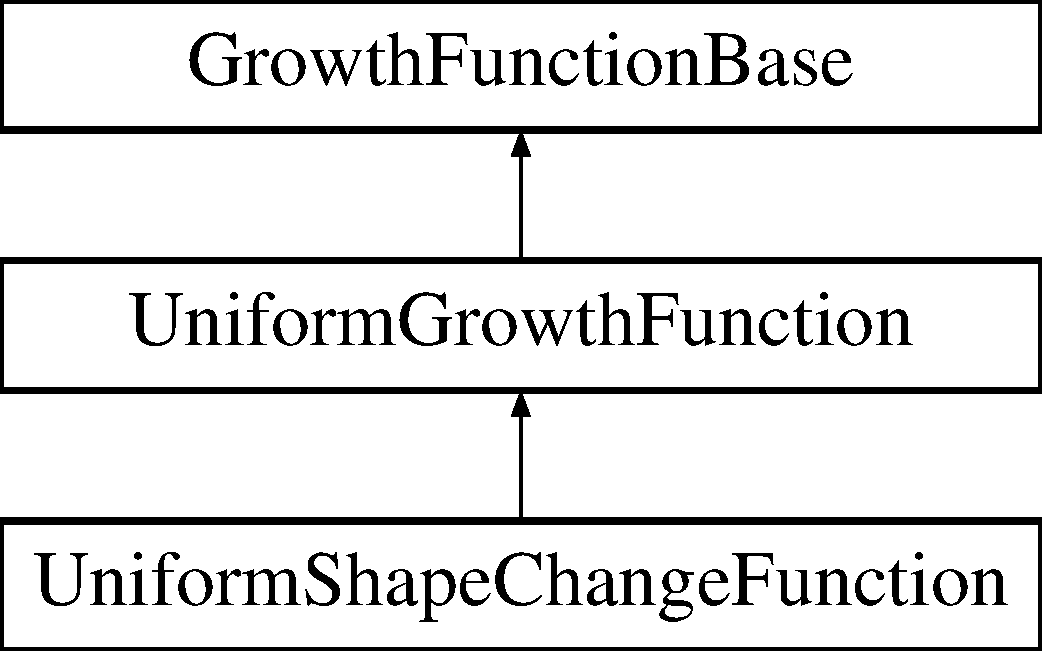
\includegraphics[height=3.000000cm]{classUniformGrowthFunction}
\end{center}
\end{figure}
\subsection*{Public Member Functions}
\begin{DoxyCompactItemize}
\item 
\hyperlink{classUniformGrowthFunction_a9ea553c72b2d5e83e98e4ec7a8c025b6}{Uniform\+Growth\+Function} (int id, int type, float \hyperlink{classGrowthFunctionBase_ae92513a7b41637df8e26e7db35ddf97c}{init\+Time}, float \hyperlink{classGrowthFunctionBase_a3ff4db0573d354a75666a5f3ca446941}{end\+Time}, bool \hyperlink{classGrowthFunctionBase_a3d56771e7c145589a14e11cc331e0326}{apply\+To\+Columnar\+Layer}, bool \hyperlink{classGrowthFunctionBase_a08ae19f58cb98fa8e315a77f52749732}{apply\+To\+Peripodial\+Membrane}, bool \hyperlink{classGrowthFunctionBase_a9fe46fc6dde4041b79204beb48972a09}{apply\+To\+Basal\+E\+C\+M}, bool \hyperlink{classGrowthFunctionBase_ac623b1dbe376bce5dddbe1a2e21c776f}{apply\+To\+Lateral\+E\+C\+M}, double D\+V\+Growth, double A\+P\+Growth, double A\+B\+Growth, double \hyperlink{classUniformGrowthFunction_a1a985ff52f9796688e00942b4d3349f8}{angle})
\begin{DoxyCompactList}\small\item\em The constructor of \hyperlink{classUniformGrowthFunction}{Uniform\+Growth\+Function}. \end{DoxyCompactList}\item 
void \hyperlink{classUniformGrowthFunction_ad5be18ae004a3eed205ab3570e13202a}{get\+Growth\+Rate} (double $\ast$max\+Values)
\begin{DoxyCompactList}\small\item\em The function is to get the 3\+D growth rate of the current growth function. \end{DoxyCompactList}\item 
void \hyperlink{classUniformGrowthFunction_aff899907569af697d47927f61b6871a5}{set\+Growt\+Rate} (double ex, double ey, double ez)
\begin{DoxyCompactList}\small\item\em The function is to set the 3\+D growth rate of the current growth function. \end{DoxyCompactList}\item 
\hypertarget{classUniformGrowthFunction_a5a7e9b102a299b94ba648513b66f9cd1}{}gsl\+\_\+matrix $\ast$ \hyperlink{classUniformGrowthFunction_a5a7e9b102a299b94ba648513b66f9cd1}{get\+Shear\+Angle\+Rotation\+Matrix} ()\label{classUniformGrowthFunction_a5a7e9b102a299b94ba648513b66f9cd1}

\begin{DoxyCompactList}\small\item\em The function return the matrix pointer to the oriented growth rotation matrix. \end{DoxyCompactList}\item 
\hypertarget{classUniformGrowthFunction_a8a60d83743c441f7453af8053d5e7010}{}double \hyperlink{classUniformGrowthFunction_a8a60d83743c441f7453af8053d5e7010}{get\+Shear\+Angle} ()\label{classUniformGrowthFunction_a8a60d83743c441f7453af8053d5e7010}

\begin{DoxyCompactList}\small\item\em The function returns the oriented growth angle in radians (double). \end{DoxyCompactList}\item 
void \hyperlink{classUniformGrowthFunction_a227ffb3a524779628f98f110d3811399}{write\+Summary} (ofstream \&save\+File\+Simulation\+Summary, double dt)
\begin{DoxyCompactList}\small\item\em The function is to write the growth function summary to simulation summary file. \end{DoxyCompactList}\end{DoxyCompactItemize}
\subsection*{Public Attributes}
\begin{DoxyCompactItemize}
\item 
\hypertarget{classUniformGrowthFunction_af78591902b0cc391a62f3093fd14ad10}{}double \hyperlink{classUniformGrowthFunction_af78591902b0cc391a62f3093fd14ad10}{Growth\+Rate} \mbox{[}3\mbox{]}\label{classUniformGrowthFunction_af78591902b0cc391a62f3093fd14ad10}

\begin{DoxyCompactList}\small\item\em The double array stating the uniform growth rate throughout the tissue. Growth rate is in 1/sec, format\+: \mbox{[} D\+V axis (x), A\+P axis (y), and A\+B axis (z)\mbox{]}. \end{DoxyCompactList}\item 
\hypertarget{classUniformGrowthFunction_afef9ac84dfe60bbf3d558fbb31946087}{}gsl\+\_\+matrix $\ast$ \hyperlink{classUniformGrowthFunction_afef9ac84dfe60bbf3d558fbb31946087}{Shear\+Angle\+Rotation\+Matrix}\label{classUniformGrowthFunction_afef9ac84dfe60bbf3d558fbb31946087}

\begin{DoxyCompactList}\small\item\em The rotation matrix for the orientation of the growth on x-\/y plane. This matrix is constructed through \hyperlink{classUniformGrowthFunction_a1a985ff52f9796688e00942b4d3349f8}{Uniform\+Growth\+Function\+::angle}. \end{DoxyCompactList}\item 
\hypertarget{classUniformGrowthFunction_a1a985ff52f9796688e00942b4d3349f8}{}double \hyperlink{classUniformGrowthFunction_a1a985ff52f9796688e00942b4d3349f8}{angle}\label{classUniformGrowthFunction_a1a985ff52f9796688e00942b4d3349f8}

\begin{DoxyCompactList}\small\item\em The rotation angle for the orientation of the growth on x-\/y plane. \end{DoxyCompactList}\end{DoxyCompactItemize}


\subsection{Constructor \& Destructor Documentation}
\hypertarget{classUniformGrowthFunction_a9ea553c72b2d5e83e98e4ec7a8c025b6}{}\index{Uniform\+Growth\+Function@{Uniform\+Growth\+Function}!Uniform\+Growth\+Function@{Uniform\+Growth\+Function}}
\index{Uniform\+Growth\+Function@{Uniform\+Growth\+Function}!Uniform\+Growth\+Function@{Uniform\+Growth\+Function}}
\subsubsection[{Uniform\+Growth\+Function}]{\setlength{\rightskip}{0pt plus 5cm}Uniform\+Growth\+Function\+::\+Uniform\+Growth\+Function (
\begin{DoxyParamCaption}
\item[{int}]{id, }
\item[{int}]{type, }
\item[{float}]{init\+Time, }
\item[{float}]{end\+Time, }
\item[{bool}]{apply\+To\+Columnar\+Layer, }
\item[{bool}]{apply\+To\+Peripodial\+Membrane, }
\item[{bool}]{apply\+To\+Basal\+E\+C\+M, }
\item[{bool}]{apply\+To\+Lateral\+E\+C\+M, }
\item[{double}]{D\+V\+Growth, }
\item[{double}]{A\+P\+Growth, }
\item[{double}]{A\+B\+Growth, }
\item[{double}]{angle}
\end{DoxyParamCaption}
)\hspace{0.3cm}{\ttfamily [inline]}}\label{classUniformGrowthFunction_a9ea553c72b2d5e83e98e4ec7a8c025b6}


The constructor of \hyperlink{classUniformGrowthFunction}{Uniform\+Growth\+Function}. 

The first six parameters will be directed to the parent constructor, \hyperlink{classGrowthFunctionBase_a5c275b3f839cc4f572b68afc5ad1064f}{Growth\+Function\+Base\+::\+Growth\+Function\+Base}. ~\newline
doubles D\+V\+Growth, A\+P\+Growth and A\+B\+Growth will set the \hyperlink{classUniformGrowthFunction_af78591902b0cc391a62f3093fd14ad10}{Uniform\+Growth\+Function\+::\+Growth\+Rate}, in the given order.

\subsection{Member Function Documentation}
\hypertarget{classUniformGrowthFunction_ad5be18ae004a3eed205ab3570e13202a}{}\index{Uniform\+Growth\+Function@{Uniform\+Growth\+Function}!get\+Growth\+Rate@{get\+Growth\+Rate}}
\index{get\+Growth\+Rate@{get\+Growth\+Rate}!Uniform\+Growth\+Function@{Uniform\+Growth\+Function}}
\subsubsection[{get\+Growth\+Rate}]{\setlength{\rightskip}{0pt plus 5cm}void Uniform\+Growth\+Function\+::get\+Growth\+Rate (
\begin{DoxyParamCaption}
\item[{double $\ast$}]{max\+Values}
\end{DoxyParamCaption}
)\hspace{0.3cm}{\ttfamily [inline]}, {\ttfamily [virtual]}}\label{classUniformGrowthFunction_ad5be18ae004a3eed205ab3570e13202a}


The function is to get the 3\+D growth rate of the current growth function. 

This function will write the \hyperlink{classUniformGrowthFunction_af78591902b0cc391a62f3093fd14ad10}{Uniform\+Growth\+Function\+::\+Growth\+Rate} of the current growth function to the input double array pointer. The double array pointer should be set to point at a double array of size 3 (or higher) before calling the fucntion.

Reimplemented from \hyperlink{classGrowthFunctionBase}{Growth\+Function\+Base}.

\hypertarget{classUniformGrowthFunction_aff899907569af697d47927f61b6871a5}{}\index{Uniform\+Growth\+Function@{Uniform\+Growth\+Function}!set\+Growt\+Rate@{set\+Growt\+Rate}}
\index{set\+Growt\+Rate@{set\+Growt\+Rate}!Uniform\+Growth\+Function@{Uniform\+Growth\+Function}}
\subsubsection[{set\+Growt\+Rate}]{\setlength{\rightskip}{0pt plus 5cm}void Uniform\+Growth\+Function\+::set\+Growt\+Rate (
\begin{DoxyParamCaption}
\item[{double}]{ex, }
\item[{double}]{ey, }
\item[{double}]{ez}
\end{DoxyParamCaption}
)\hspace{0.3cm}{\ttfamily [inline]}, {\ttfamily [virtual]}}\label{classUniformGrowthFunction_aff899907569af697d47927f61b6871a5}


The function is to set the 3\+D growth rate of the current growth function. 

This function will set the \hyperlink{classUniformGrowthFunction_af78591902b0cc391a62f3093fd14ad10}{Uniform\+Growth\+Function\+::\+Growth\+Rate} of the current growth function to the input values The parameters are in the order \mbox{[} D\+V axis (x), A\+P axis (y), and A\+B axis (z)\mbox{]}.

Reimplemented from \hyperlink{classGrowthFunctionBase}{Growth\+Function\+Base}.

\hypertarget{classUniformGrowthFunction_a227ffb3a524779628f98f110d3811399}{}\index{Uniform\+Growth\+Function@{Uniform\+Growth\+Function}!write\+Summary@{write\+Summary}}
\index{write\+Summary@{write\+Summary}!Uniform\+Growth\+Function@{Uniform\+Growth\+Function}}
\subsubsection[{write\+Summary}]{\setlength{\rightskip}{0pt plus 5cm}void Uniform\+Growth\+Function\+::write\+Summary (
\begin{DoxyParamCaption}
\item[{ofstream \&}]{save\+File\+Simulation\+Summary, }
\item[{double}]{dt}
\end{DoxyParamCaption}
)\hspace{0.3cm}{\ttfamily [inline]}, {\ttfamily [virtual]}}\label{classUniformGrowthFunction_a227ffb3a524779628f98f110d3811399}


The function is to write the growth function summary to simulation summary file. 

This function will write the \hyperlink{classUniformGrowthFunction}{Uniform\+Growth\+Function} details into the simulation summary file, provided as the first input. Time step (dt) of the simulation is provided as second input, to report the growth rates per hour. The output should look like\+: ~\newline
 Growth Type\+: Uniform (1) Initial time(sec)\+: \hyperlink{classGrowthFunctionBase_ae92513a7b41637df8e26e7db35ddf97c}{Uniform\+Growth\+Function\+::init\+Time} Final\+Time time(sec)\+: \hyperlink{classGrowthFunctionBase_a3ff4db0573d354a75666a5f3ca446941}{Uniform\+Growth\+Function\+::end\+Time} Growth\+Rate(fraction/hr)\+: D\+V\+Growth(in 1/hr) A\+P\+Growth(in 1/hr) A\+B\+Growth(in 1/hr)

Reimplemented from \hyperlink{classGrowthFunctionBase}{Growth\+Function\+Base}.



Reimplemented in \hyperlink{classUniformShapeChangeFunction_a196a7555899800406ee62714a20b34c4}{Uniform\+Shape\+Change\+Function}.



The documentation for this class was generated from the following file\+:\begin{DoxyCompactItemize}
\item 
/home/melda/\+Documents/\+Tissue\+Folding/\+Tissue\+Folding/\+Source\+Code/Growth\+Function\+Types.\+h\end{DoxyCompactItemize}

%--- End generated contents ---

% Index
\backmatter
\newpage
\phantomsection
\clearemptydoublepage
\addcontentsline{toc}{chapter}{Index}
\printindex

\end{document}
